\documentclass[compontinhos,showtrims,trimframe,12pt,conselho,spreadimages]{memoir}

\usepackage[Kalinka]{hedraoptions} %% << %%%%%%%%%%%%%%%%
\usepackage[baruch]{hedrastyles}
\usepackage[xetex,chicagofootnotes]{tipografia}
\usepackage[standart,sempontinhos]{toc}
\usepackage{hedraextra}
\usepackage{penalidades}
\usepackage{graficos}
\usepackage{hedralogo}
\usepackage{hifensextras}
\usepackage{fichatecnica}
\usepackage{tocloft}
\usepackage[standart]{aparatos}
\usepackage{tabelas}
\usepackage{versos}
\usepackage{gitrevisioninfo}

\newcommand{\forceindent}{\leavevmode{\parindent=1,4em\indent}}


%---------------------------------------ÍNDICE ONOMÁSTICO
\usepackage{imakeidx} 
\makeindex[program=xindy, options=-C utf8 -L portuguese]
%---------------------------------------MANCHA DE TEXTO AO LADO DE IMAGEM
\usepackage{wrapfig}
%---------------------------------------NUMERAÇÃO DE PAGINA NAS LATERAIS
\usepackage{graphicx}
\usepackage{fancyhdr}
\pagestyle{fancy}
\fancyhf{}
\fancyfoot[LE,RO]{\Georgia \scriptsize \thepage}
\renewcommand{\headrulewidth}{0pt}

%---------------------------------------NUMERAÇÃO NAS LATERAIS EM CHAPTER
\fancypagestyle{chapter}{
\fancyhf{}
\fancyfoot[RO]{\Georgia \scriptsize \thepage}
\renewcommand{\headrulewidth}{0pt}
\renewcommand{\footrulewidth}{0pt}}

%---------------------------------------GERAR BLANK PAGE
\usepackage{afterpage}

\newcommand\blankpage{%
    \null
    \thispagestyle{empty}%
    \addtocounter{page}{0}%
    \newpage}
%---------------------------------------MUDAR FONTE DE PART
\usepackage{titlesec}
\titleformat{\part}
[display]
{\Huge\bfseries\BebasNeue}
 {\huge\parttitlename\space\thepart}
  {20pt}
  {\centering\thispagestyle{empty}}

%---------------------------------------MUDAR FONTE DE CHAPTER
\titleformat{\chapter}
[display]
{\Large\bfseries\MyriadPro}
 {\large\chaptertitlename\space\thechapter}
  {20pt}
  {\centering}

\titleformat{\section}
[display]
{\small\MyriadPro}
 {\small\sectiontitlename\space\thesection}
  {20pt}
  {\centering}

%-----------------------------------PARA INCLUIR IMAGEM NA PART
%\usepackage{epigraph}
%\setlength{\epigraphwidth}{\textwidth}
%\titleformat{\part}[display]
%{\Huge\bfseries\BebasNeue\thispagestyle{epigraph}}
%{\partname\ \thepart}
%{20pt}
%{\Huge}
%{\centering}
%\titlespacing*{\part}{0pt}{0pt}{40pt}
%----------------------------------------TIRAR O DIVISOR DE NOTA DE RODAPÉ E CORPO DO TEXTO

\usepackage{footmisc}

\renewcommand*\footnoterule{}

%---------------------------------------DEFINIR FONTES SECUNDÁRIAS
%\usepackage[utf8]{inputenc}
%\usepackage{MyriadPro}
%\setsansfont{MyriadPro}
%\renewcommand{\familydefault}{\sfdefault}
%\DeclareTextFontCommand{\textmyfont}{MyriadPro}
%\newfontfamily\MyriadPro[Ligatures=TeX]{MyriadPro-Regular}
%\newfontfamily\MyriadPro[Ligatures=TeX]{MyriadPro-Light}
\newcommand{\slsc}[1]{\fontspec[SmallCapsFeatures={FakeSlant=0.6}]{MyriadPro-LightIt}\textsc{#1}\fontspec[]{MyriadPro-LightIt}}

\newfontfamily\MyriadPro{MyriadPro-Regular}[
ItalicFont = MyriadPro-Light]	
%\newfontfamily\BebasNeue[Ligatures=TeX]{BebasNeue-Regular}	
\newfontfamily\MinionPro[Ligatures=TeX]{MinionPro-Regular}	
\newfontfamily\Georgia[Ligatures=TeX]{Georgia}	
%---------------------------------------DEFINIR FONTE PRIMÁRIA
%\setmainfont{MyriadPro-Regular.otf}
\usepackage{fontspec}
\setmainfont[Ligatures=TeX]{Adobe Devanagari}
%--------------------------------------- FOOTNOTE NO FINAL DO LIVRO
\usepackage{endnotes}
\renewcommand{\notesname}{Notas}

%\counterwithin*{endnote}{part}
%\counterwithin*{endnote}{chapter}

\let\latexchapter\chapter
\makeatletter
\renewcommand\enoteheading{%
  \setcounter{secnumdepth}{-2}
  \latexchapter*{\notesname\markboth{NOTAS}{}}
  \mbox{}\par\vskip-\baselineskip
  \let\@afterindentfalse\@afterindenttrue
}
\makeatother


\usepackage{xparse}


\let\latexchapter\chapter

\RenewDocumentCommand{\chapter}{som}{%
  \IfBooleanTF{#1}
    {\latexchapter*{#3}}
    {\IfNoValueTF{#2}
       {\latexchapter{#3}}
       {\latexchapter[#2]{#3}}%
     \addtoendnotes{\unexpanded{\enotedivision{\subsection}{#3}}}
    }
}
\makeatletter
\def\enotedivision#1#2{\@ifnextchar\enotedivision{}{#1{#2}}}
\makeatletter

%\linespread{1.08}
\usepackage{commands}

\usepackage{setspace}

\usepackage{multirow}

\makeatletter
\newenvironment{Parskip}{%
   \par
   \parskip=0.2\baselineskip \advance\parskip by 0pt plus 2pt
   \parindent=\z@
   \def\@listI{\leftmargin\leftmargini
      \topsep\z@ \parsep\parskip \itemsep\z@}
   \let\@listi\@listI
   \@listi
   \def\@listii{\leftmargin\leftmarginii
      \labelwidth\leftmarginii\advance\labelwidth-\labelsep
      \topsep\z@ \parsep\parskip \itemsep\z@}
   \def\@listiii{\leftmargin\leftmarginiii
       \labelwidth\leftmarginiii\advance\labelwidth-\labelsep
       \topsep\z@ \parsep\parskip \itemsep\z@}
   \partopsep=\z@
}{\par}
\makeatother

\makeatletter
\newenvironment{myParskip}{%
   \par
   \parskip=0.2\baselineskip \advance\parskip by 0pt plus 2pt
   \parindent=\z@
   \def\@listI{\leftmargin\leftmargini
      \topsep\z@ \parsep\parskip \itemsep\z@}
   \let\@listi\@listI
   \@listi
   \def\@listii{\leftmargin\leftmarginii
      \labelwidth\leftmarginii\advance\labelwidth-\labelsep
      \topsep\z@ \parsep\parskip \itemsep\z@}
   \def\@listiii{\leftmargin\leftmarginiii
       \labelwidth\leftmarginiii\advance\labelwidth-\labelsep
       \topsep\z@ \parsep\parskip \itemsep\z@}
   \partopsep=\z@
}{\par}
\makeatother

\newcommand{\mystar}{{\fontfamily{lmr}\selectfont$\star$}}

\hyphenation{khris-tianin}
\hyphenation{Via-tches-láv}
\hyphenation{Schnai-derman}
\hyphenation{Kru-tchónykh}
\hyphenation{Tiú-tchev}
\hyphenation{Khléb-nikov}
\hyphenation{Dobý-tchin}
\hyphenation{Petri-tchen-ka}
\hyphenation{bio-grafia}
\hyphenation{in-quie-to}
\hyphenation{moe-da}
\hyphenation{poe-mas}
\hyphenation{pen-sio-nis-tas}
\hyphenation{da-tcha}
\hyphenation{Mú-rom-tsev}
%\usepackage{ogonek}
%\makeatletter
%\renewcommand{\@chapapp}{}% Not necessary...
%\newenvironment{chapquote}[2][2em]
%  {\setlength{\@tempdima}{#1}%
%   \def\chapquote@author{#2}%
%   \parshape 1 \@tempdima \dimexpr\textwidth-2\@tempdima\relax%
%   \itshape}
%  {\par\scriptsize\hfill-- \chapquote@author\hspace*{\@tempdima}\par\bigskip}
%\makeatother

%\newcommand\Chapter[2]{\chapter
%  [#1\hfil\hbox{}\protect\linebreak{\itshape#1}]%
%  {#1\\[2ex]\Large\itshape#2}%
%}

%\usepackage{graphicx,eso-pic,etoolbox}
%\providecommand{\parthook}{}
%\patchcmd{\part}{\thispagestyle}{\parthook\thispagestyle}{}{}
%\newcommand{\partimage}[2][]{% \parthook[<options>]{<image>}
%  \renewcommand{\parthook}{% Update \parthook
%    \AddToShipoutPictureBG*{% Add picture to background of THIS page only
%      \AtPageLowerLeft{\includegraphics[width=\paperwidth,height=\paperheight,#1]{#2}}}% Insert image
%    \renewcommand{\parthook}{}}}% Restore \parthook

\begin{document}

%!TEX root=./LIVRO.tex
{\setlength\parindent{0pt}\thispagestyle{empty}


\begin{vplace}
\begin{centering}
\textbf{Prefácio}

\medskip

p. 0\pageref{prefacio}

\medskip

\textbf{A cidade Ene}

\medskip

p. \pageref{cidade}

\medskip

\textbf{Colaboradores}

\medskip

p. \pageref{colaboradores}

\end{centering}
\end{vplace}

\pagebreak
\thispagestyle{empty}
}
\pagebreak
\thispagestyle{empty}


\begin{vplace}[.8]
\begin{center}
\label{cidade}
{\MyriadPro{A Cidade Ene}}
\end{center}
\end{vplace}

%\vfill
%\hfill
%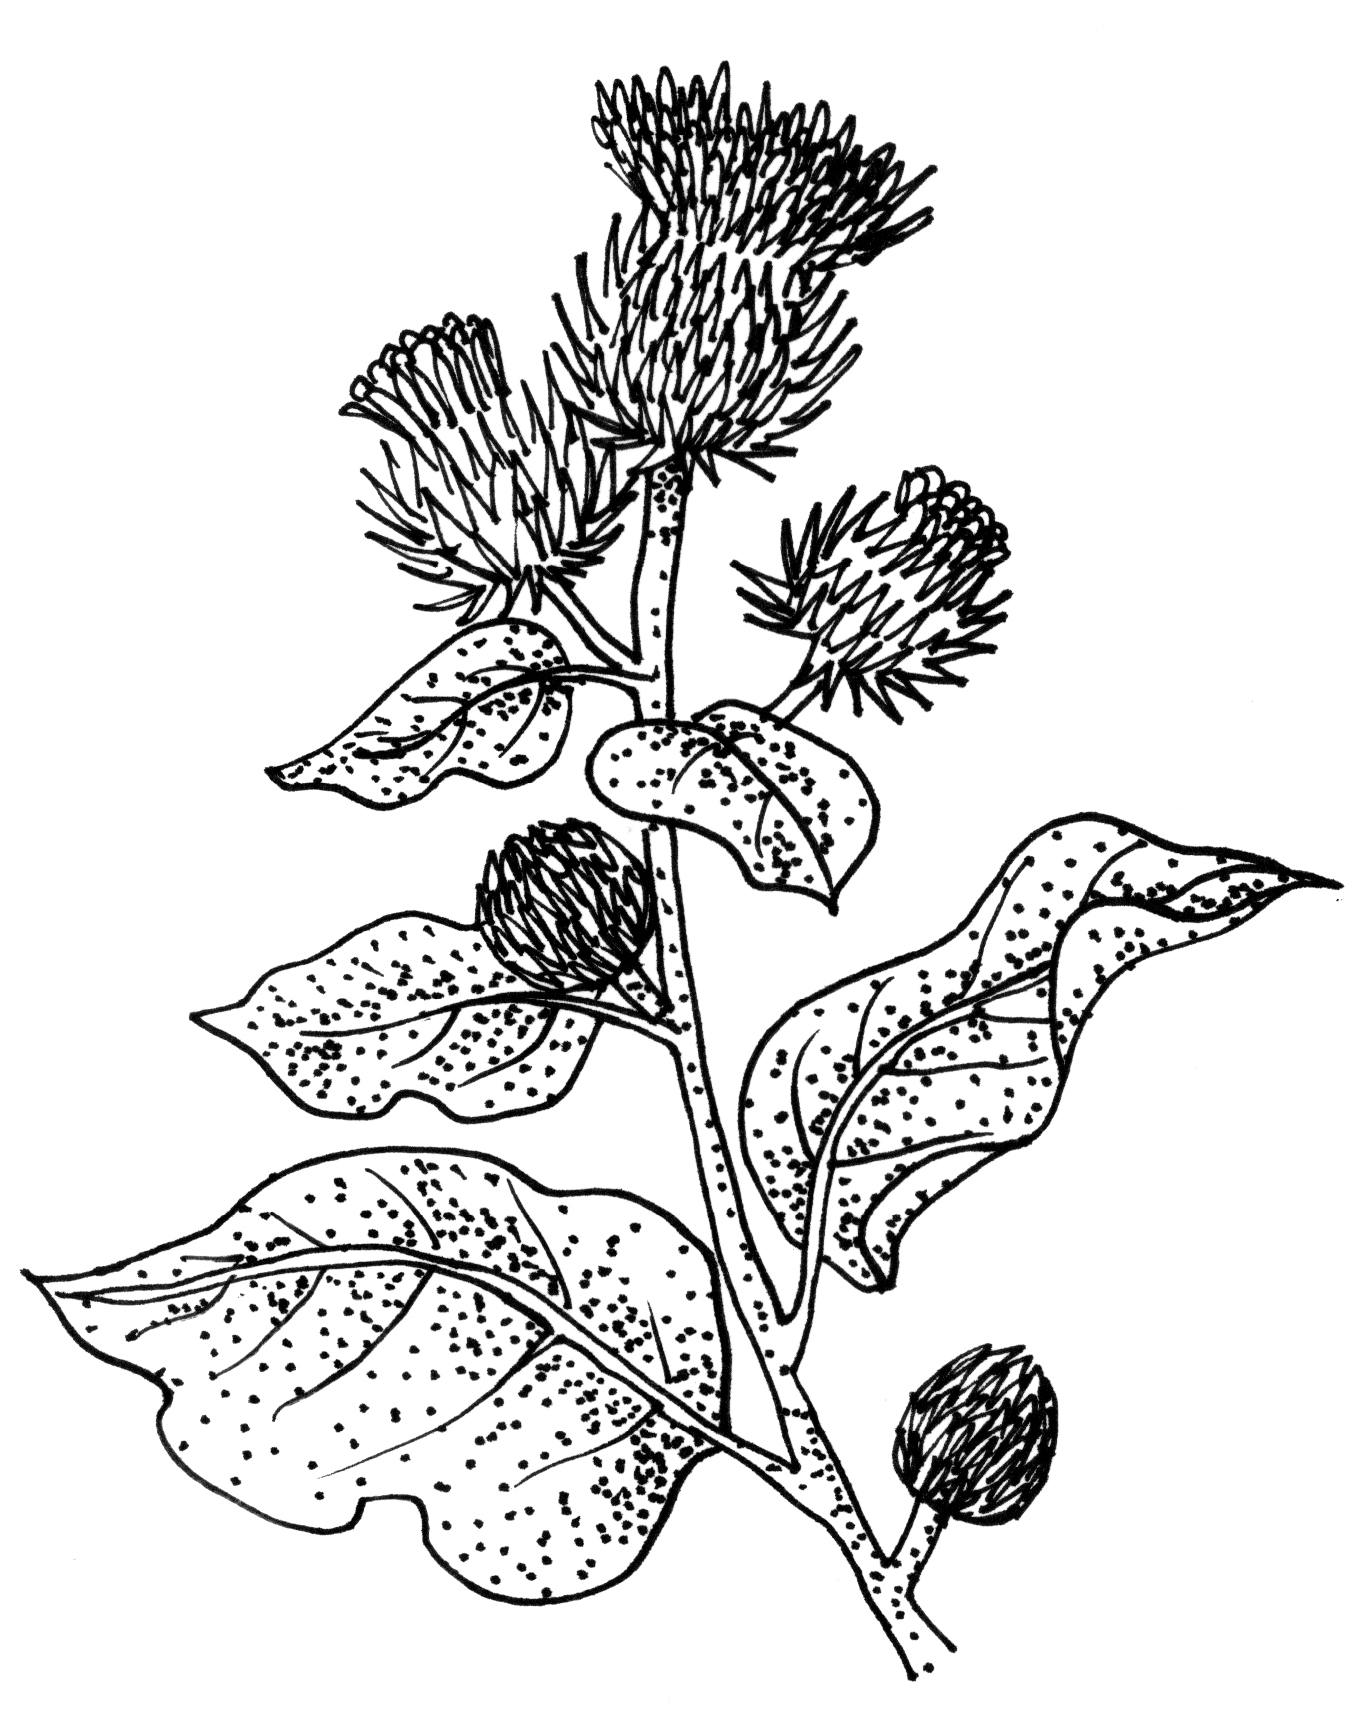
\includegraphics[width=4.5cm]{./bordo.jpg}

\pagebreak

\begin{vplace}[30]
\begin{flushright}
\emph{A Aleksandr Pávlovitch Drozdóv}
\end{flushright}
\end{vplace}
\thispagestyle{empty}


\section{1} 

Chuviscava. As barras da roupa de \emph{maman} e de Aleksandra Lvovna
Lei estavam erguidas e em alguns lugares fixas, com fivelas, em tiras de
elástico que eram costuradas num cinto de borracha. Chamavam esses
elásticos de \emph{pajens}. As pedras molhadas do pavimento das ruas e
os tijolos das calçadas brilhavam. Gotas caíam dos guarda"-chuvas. Nas
tabuletas das lojas, índios marrons e nus, com penas na cabeça, fumavam.
--- Não olhe para trás --- \emph{maman} me dizia.

O castelo"-prisão, de quatro andares, com torres, podia ser visto
adiante. Lá celebravam o dia da Nossa Senhora dos Aflitos, e nós
estávamos indo para a missa. Aleksandra Lvovna Lei dava lições de moral
e \emph{maman}, enternecida, assentia.

--- No fim das contas --- diziam elas ---, seria difícil encontrar lugar
mais apropriado para essa festa do que a prisão.

Assoando o nariz, uma dama imponente com uma gola de pele nos
ultrapassou e, aproximando o pincenê dos olhos, lançou"-nos um olhar
benevolente. Seu rosto moreno lembrava uma imagem de
Tchítchikov.\footnote{Tchítchikov, personagem principal de \emph{Almas
  mortas} (1842), de Nikolai Gógol (1809--1852).} Nos portões
todos se detiveram para desafivelar os \emph{pajens}, e a
dama"-Tchítchikov nos olhou mais uma vez. De suas orelhas pendiam brincos
de pedra marrom com brilhos. --- Charmosa --- disse \emph{maman}.

Nós entramos na igreja e nos apinhamos em frente à caixa de velas. --- É
para a \emph{proskomidia}\footnote{\emph{Proskomidia}, primeira parte da
  liturgia ortodoxa.} --- senhoras balbuciaram separando moedinhas. Pope
Fiódor, em um traje dourado com ramalhetes azuis, saudando"-nos, meneava
o turíbulo em nossa direção. Fiquei lisonjeado por ter nos recebido tão
gentilmente. Atrás do castelo passava a estrada de ferro e se ouviam
apitos. Na iconóstase eu reparei em Nossa Senhora. Ela não era
descarnada e escura, mas cheiinha, e seu lenço esvoaçava lindamente em
suas costas. Ela me agradou. Os prisioneiros nos fitavam do coro. ---
Endireite"-se --- \emph{maman} me ordenou.

Ouviu"-se um tropel e, fazendo o sinal da cruz, apareceram as alunas. Uma
professora as enfileirou. Fez o sinal da cruz e, ajeitando a saia por
trás, olhou"-a de relance. Depois, semicerrando os olhos, avistou"-nos e
nos cumprimentou. --- \emph{Madmaselle}\footnote{\emph{Madmaselle},
  russificado do francês (corruptela).} Gorchkova --- esclareceu
Aleksandra Lvovna, fazendo"-lhe um aceno de cabeça. A dama"-Tchítchikov de
tempos em tempos dirigia"-nos o olhar.

De repente um guarda da prisão trouxe o leitoril e deu um tossido. Todos
se aproximaram. Pope Fiódor apareceu limpando o nariz com um lencinho.
Deu"-se um ar de importância e fez um sermão a respeito das aflições.

--- Não se deve evitá"-las --- dizia ele. --- Deus nos visita por meio
delas. Um santo que não tinha aflições pôs"-se a chorar amargamente:
``Deus me esqueceu'', afligia"-se ele.

--- Ah, como isso é verdadeiro --- admiravam"-se as mulheres atravessando
o portão e entretendo"-se novamente com os \emph{pajens}. A chuva amainou
um pouco. \emph{Madmaselle} Gorchkova nos alcançou. Aleksandra Lvovna
Lei nos apresentou a ela. As alunas nos rodearam e, ao serem enxotadas
por \emph{madmaselle} Gorchkova, afastavam"-se correndo e então voltavam
aos saltinhos. Eu me senti indignado.

Assim paramos por alguns minutos. Locomotivas apitavam. Pope Fiódor
subiu num \emph{drójki}\footnote{\emph{Drójki}, do russo, carruagens
  leves, para distâncias curtas.} e, tocando nas costas do cocheiro,
partiu. Nós ficamos conversando. Aleksandra Lvovna Lei gesticulava e se
expressava com voz grave e monótona. --- Verdade, verdade ---
\emph{maman} concordava com ela, agitando de vez em quando o chapéu.
\emph{Madmaselle} Gorchkova agasalhava"-se no boá de plumas, erguia as
sobrancelhas e semicerrava os olhos. Seu olhar retinha"-se em mim e uma
ideia faiscou em seu rosto. Eu fiquei inquieto. Nesse meio"-tempo, a
dama"-Tchítchikov chegou até a esquina, lançou um olhar para trás e
desapareceu.

Após nos despedirmos de \emph{madmaselle} Gorchkova falamos dela. ---
Bem"-educada --- a elogiamos e, entrando na rua principal, nos calamos.
Rodas troavam. Vendeiros, parados nas soleiras, atraíam"-nos para dentro.
--- Vamos dar um pulinho ali --- disse repentinamente \emph{maman} e nós
entramos na livraria L. Kusman. Lá, à meia"-luz, sentia"-se o cheiro
agradável dos globos e das encadernações. A lânguida L. Kusman nos
fitava tristemente com olhos inexpressivos. --- Eu vejo a senhora tão
raramente --- disse ela, afável. --- Dê"-me \emph{A história sagrada} ---
pediu \emph{maman}. Todos se viraram e fixaram os olhos em mim.

L. Kusman me fez um sinal com os olhos, enfiou uma figura na
\emph{História sagrada}, embrulhou agilmente a encomenda e a entregou.
--- Um rublo e dez --- anunciou ela o preço e depois disse: --- Para a
senhora, um rublo.

Descobriu"-se que era a figura de um ``anjo''. Coberto de verniz, tinha
umas saliências. \emph{Maman} o colou na sala, no papel de parede. ---
Para que ele faça você comer como se deve --- disse ela. Durante as
refeições, eu não tirava os olhos dele. --- Que encantador --- pensava
eu amorosamente.

\section{2}

O pai saiu para a repartição onde recebiam os recrutas. \emph{Maman},
ainda não arrumada, ocupava"-se com a faxina. Eu peguei um livro e li
como Tchítchikov chegou à cidade Ene\footnote{Referência à cidade N para
  onde vai Tchítchikov em \emph{Almas mortas.}} e a todos agradou.
Como atrelaram sua sege, como foram visitar os proprietários rurais, e o
que comeram lá. Como Manílov\footnote{Manílov, primeiro proprietário
  visitado por Tchítchikov, em \emph{Almas mortas. }} se afeiçoou a ele
e, parado no \emph{kryltsó},\footnote{\emph{Kryltsó}, do russo, escada
  externa na entrada das casas, com ou sem cobertura.} sonhou que o tsar
tomaria conhecimento da amizade entre eles e lhes concederia o título de
general.

--- Com o que está se distraindo? --- perguntou \emph{maman}. Ela sempre
falava assim, em vez de: ``o que está lendo?''. --- Chame Cecília ---
disse ela --- e vá passear. --- Cecília --- eu gritei e ela apareceu num
instante, baixinha. Pegou o avental e abriu seu bauzinho, que apelidou
de \emph{skrynka}.\footnote{\emph{Skrynka}, ``baú'' no russo antigo.}
Uma musiquinha soou no fecho e apareceu o papa Leão \scalebox{.8}{XIII}. Ele havia sido
colado no interior da tampa.

O dia estava ensolarado e a rua resplandecia. Uma ovelha de chocolate
brilhava na janela da padaria. Telegas troavam. Conversando, éramos
obrigados a gritar para escutar um ao outro. Ficamos admirados com a
senhora da janela da barbearia, e apreciamos os objetos religiosos da
janela do Piotr Mitrofánov \& Cia. Uma marcha troou. Um pelotão se
aproximava e a orquestra tocava, reluzindo. O regente Schmidt agitava
majestosamente a mão enluvada. Madame Strauss, num vestido vermelho,
saiu a toda da salsicharia e, sorrindo com deleite, ficou acenando para
ele com a cabeça. L. Kusman cobriu"-se com um xale e entreabriu a porta.

Ouviu"-se um canto estridente e surgiu uma procissão fúnebre. Um homem de
camisa de renda carregava uma cruz, um padre andava à frente, cheio de
si. --- Lá --- disse Cecília com devoção e olhou para o alto --- as
babás e as cozinheiras serão soberanas, e os senhores irão servi"-las. Eu
não acreditava nisso.

--- Aqui parece uma boa travessa --- disse Cecília. Nós viramos e
avistamos o \emph{kostiol}.\footnote{\emph{Kostiol}, palavra russa de origem polonesa, templo católico. Poloneses são, na maioria, católicos.} De telhado vermelho, o templo embranquecia atrás dos
galhos. Junto à cerca, que em semicírculo recuava da rua, pedintes
estavam sentados. Cecília aproveitou a ocasião e nós entramos. Já estava
vazio, mas ainda se sentia o cheiro dos devotos. Perto da entrada, havia
duas mulheres de pedra e uma delas lembrava L. Kusman e estava coberta
de panos como ela. Nós rezamos a elas e ficamos andando em silêncio.
Passos ressoavam. --- A nossa crença é a verdadeira --- gabava"-se
Cecília enquanto saíamos. Eu não concordava.

Do outro lado da rua, eu vi numa janela um rapazinho moreno e cutuquei
Cecília. Nós paramos e o observamos. De repente ele envesgou os olhos,
enfiou os dedos nos cantos da boca e, puxando"-os para baixo, meteu a
língua para fora. Dei um grito de medo. Cecília tapou meu rosto com a
palma da mão. --- Cuspa --- ela me ordenou e fez o sinal da cruz: ---
Jesus, Maria, José. Nós demos no pé.

--- ``Um menino terrível'' --- assim o pai rotulou o acontecido.
\emph{Maman} olhou para ele com desgosto. Ela preferia que levassem tudo
a sério.

Já fazia três dias que Aleksandra Lvovna Lei não aparecia, e durante o
almoço nós falamos dela. Resolvemos que ela estava ``em atendimento''. A
mim deram duas porções extras de \emph{kissiel},\footnote{\emph{Kissiel},
  do russo, espécie de gelatina de frutas engrossada com amido de batata
  e servida com creme.} para que minhas forças, abaladas pelo susto,
fossem restabelecidas rapidamente. Na parede diante de mim estava o anjo
de L. Kusman. Com um ramo de palmeira, ele postava"-se numa nuvem. Uma
estrela brilhava sobre sua cabeça.

Przyborowski, o enfermeiro, deu o ar de sua graça. Com os cabelos em pé
e os bigodes largos, ele lembrava um retrato de ``Nietzsche''. Ao
levantar, meu pai mandou"-o limpar os instrumentos e saiu do quarto. ---
Vai para os braços de Morfeu --- esclareceu com respeito Przyborowski,
fazendo uma reverência a suas costas. --- Acomode"-se aqui --- ordenou
\emph{maman}, à mesa. --- Não vale a pena acender outra lâmpada. --- É
pura verdade --- respondeu Przyborowski.

Pinças e tesouras variadas começaram a brilhar. --- Hoje --- falava ele
ao limpá"-las --- calhei de passar no \emph{kostiol}. O sermão foi
excelente --- e ele o descreveu: --- Como devemos obedecer, cumprir com
os deveres. --- Está correto --- \emph{maman} concordou com indulgência
e ficou pensativa. --- Afinal, Deus é apenas um --- disse ela ---, as
crenças é que são diferentes. --- Exatamente --- comoveu"-se
Przyborowski. Ele estava radiante.

Aleksandra Lvovna Lei nos surpreendeu entretidos nessa reflexão. Ficamos
contentes, esquentamos o almoço para ela, perguntamos quem havia
nascido. Às sete horas, já pronto para dormir, eu fechei os olhos. De
repente aquele menino terrível surgiu diante de mim. Eu pulei da cama.
As mulheres vieram correndo, alvoroçadas, e ficaram sentadas ao meu
lado, falando baixinho, até que eu adormecesse. --- Não, mas
Léikin\ldots{}\footnote{Nikolai Léikin (1841--1906), escritor humorista
  russo. Editou a revista de humor \emph{Oskólki} (1881--1916), em
  que Tchékhov começou a publicar.} --- eu ouvia ao pegar no sono. ---
Vocês leram como eles se perderam em Paris, então contrataram um
cocheiro e lhe deram o endereço? --- e elas riam aos cochichos.

\section{3}

A neve deitou"-se nas pedras do pavimento. Tudo estava em silêncio. Nós
mandamos embora Cecília. Ela ofendia nossa religião e isso chegou ao
conhecimento de \emph{maman}.

O fecho da \emph{skrynka} tocou sua música, o papa Leão apareceu mais
uma vez --- com um solidéu e uma pelerine. Comovido, resolvi despedir"-me
de Cecília amigavelmente e oferecer"-lhe pão com sal.\footnote{Antigo
  costume russo, o pão com sal é oferecido como boas"-vindas.} Salpiquei
sal em um naco de pão e o estendi para ela, mas ela o empurrou.

Kágan, a agenciadora, enviou"-nos uma nova babá. Ela era uniata\footnote{Uniata
  é um adepto de uma das igrejas católicas orientais, chamadas greco"-católicas ou católicas bizantinas, que, mantendo
  liturgias e hierarquias próprias, submetem"-se ao poder do papa. O termo ``uniata'' é hoje considerado pejorativo por greco"-católicos, achados sobretudo na Ucrânia, mas também na Bielorrússia e na Romênia, entre outros.} e
isso agradou a todos. --- Existe até uma medalha --- falavam os
convidados --- em homenagem à extinção da União. Chegou o natal.
\emph{Maman} sorria e parecia contente. --- Tenho recordações da
infância --- repetia ela.

Ela havia sido convidada para passar o ano"-novo na casa dos Belúguin.
Com os cabelos frisados em um penteado incomum, ela se postava ereta na
frente do espelho. Duas velas a iluminavam. Subindo na cadeira, eu
afivelei os ganchinhos de seu vestido. O pai já estava de sobrecasaca.
Ele nos borrifava com o perfume do pulverizador. --- Minha alma está
radiante --- aproximando"-se dele e pegando sua mão, disse \emph{maman}.
--- Por que motivo? Será que ganhamos duzentos mil?

Após ser despido pela babá, eu ponderei sobre o que poderíamos fazer com
esse dinheiro. Nós compraríamos uma sege e rodaríamos a cidade de Ene.
Todos nos amariam. Eu faria amizade com Femistoklius e Alkid
Manílov.\footnote{Femistoklius, de 8 anos, e Alkid, de 6 anos, filhos de
  Manílov, em \emph{Almas mortas}.}

A manhã estava agradável. Da repartição vinham vigilantes, limpadores de
chaminés e funcionários das casas de banho e nos felicitavam pelo ano"-novo. --- Muito bem, muito bem --- nós falávamos e distribuíamos moedas
de um rublo. O carteiro trouxe uma pilha de cartões"-postais e de
envelopes com cartões de visita: orquestras de anjos tocavam violinos,
homens de fraque e damas de cauda brindavam, coroas foram impressas sobre
os nomes e os patronímicos de nossos conhecidos.

\emph{Maman}, sorrindo, sentou"-se ao meu lado. --- Hoje à noite ---
disse ela --- fui apresentada a uma senhora que tem um menino de nome
Serge. Vocês serão amigos. Amanhã ele virá para cá. Ela se levantou.
Olhou o termômetro do lado de fora e mandou a babá me levar para
passear.

Cheirava a neve. Corvos gritavam. Os rocinantes dos cocheiros corriam
sem pressa. Caíam pingos dos telhados. --- De repente é Serge --- eu e a
babá conversávamos sobre os meninos que nos agradavam. O gordo Strauss,
vestindo uma jaqueta cinza e um chapeuzinho com uma pena verde, passou
em disparada. Com uma mão ele guiava o trenó, a outra ele mantinha na
cintura de madame Strauss. A catedral repicava, e todos se dirigiam
naquela direção --- para ver a parada.

Atravessando a multidão, encontramos lugares. Soldados batiam com os pés
no chão. Policiais em cavalos enormes abriam caminho, afastando as
pessoas. Sinos começaram a repicar. Todos se animaram. Nas portas,
apareceram estandartes inclinados e logo endireitados. Celebraram o
te"-déum. A parada pôs"-se em marcha. Alguém deu um piparote na minha
nuca. Era um aluno usando um sobretudo com botões dourados. Mas ele já
não prestava atenção em mim. Com a cabeça erguida, observava o movimento
das nuvens de chuva. Ele lembrava nosso anjo (no papel de parede da
sala) e eu fiquei enternecido. --- Tão querido --- pensava eu.

Voltamos a passos militares, acompanhados pelos sons da música que se
afastava. O pai, que tinha passado em vários lugares para dar
felicitações, topou conosco. Ele me acomodou no trenó e me levou para
casa. A babá nos seguiu correndo.

Quando chegamos, um convidado estava sentado no sofá da sala. Com sua
postura ereta, \emph{maman} o recebia. Ele fazia girar nas mãos o
cinzeiro ``Dreyfus está lendo uma revista'' e contava que em Petersburgo
tinham aparecido pneus de borracha. --- Você caminha --- dizia ele --- e
nota como os \emph{drójki} deslizam sem ruído.

Durante o almoço, sentimos falta de Aleksandra Lvovna. Mandamos
Przyborowski atrás dela, mas ela, pobrezinha, estava em atendimento.

À noite tivemos visitas e lhes contamos sobre os pneus de borracha. ---
Os progressos da ciência --- admiraram"-se. Barbudos como na
\emph{História sagrada}, eles sentaram para jogar baralho. No meio
deles, o pai parecia um jovenzinho. --- Passo --- anunciavam. Um deles
estava ``fora'', e \emph{maman} o entretinha. --- Ontem eu conheci ---
dizia ela --- a esposa do engenheiro Karmánov. Uma mulher muito
agradável. Não me arrumei à toa para ir à casa dos Belúguin, eu estava
cheia de pressentimentos alegres. Ela irá nos visitar amanhã. --- E
Serge também --- acrescentei eu.

Finalmente chegou a hora da visita. A campainha tocou. Eu saí correndo.
Uma lâmpada iluminava a antessala. \emph{Maman} já se perdia em
exclamações. Diante dela, assoando o nariz e livrando"-se de suas
peliças, surgiram sorrindo a dama"-Tchítchikov e o ``menino terrível''.

\section{4}

O anjo da sala de jantar agradou a todos. A mulher do engenheiro o
examinou detidamente através de seu pincenê e disse que ele era
estrangeiro. Eu me alegrei. Ela lançou ao redor um olhar benevolente.
Vestia um casaquinho de veludo azul cheio de brilho, o broche ``comunhão
de amor'', e um cinto com uma fivela em forma de lira. --- Frequentam a
fortaleza? --- perguntou ela: --- Aos sábados organizam acatistos lá.

Serge trajava um terninho verde. Ele pegou"-me pela mão e, levando"-me
para o lado, mostrou que o fecho de suas calças tinha sido colocado na
frente.

--- É como os adultos --- disse eu, fascinado. Conversamos um pouco. ---
Serge --- olhando ao redor, eu perguntei ---, foi você que um dia me fez
uma careta? --- ele jurou que não. Senti"-me tocado.

O pai apareceu para o chá após as visitas terem partido. Muito
satisfeita, \emph{maman} cantarolava e, com ar de malícia, dava
risadinhas. --- Sabe --- disse ela ---, nós combinamos reler Léikin
juntas.

Eu também estava feliz. Deixei"-os e passei sem ser percebido para a
sala. Lá eu me ajeitei perto da estufa, ouvindo as agulhas de abeto
caírem. Através da janela, um lampião iluminava um galho de abeto. Uma
chuvinha prateada reluzia nele. --- Serge, Serge, ah, Serge --- repetia
eu.

Depois eu e \emph{maman} fomos visitá"-los. Trocamos beijinhos na
antessala. A esposa do engenheiro nos apresentou a sua filha, a
ginasiana Sophie Samokvássova. --- Muito prazer --- disse Sophie.
Enlaçando"-se pela cintura, as damas passaram para o quarto da anfitriã
que ela chamava \emph{boudoir}. Eu apertei a mão de Serge: --- Eu e você
somos como Manílov e Tchítchikov. Ele não tinha lido nada sobre eles. Eu
lhe contei como ficaram amigos e como queriam morar juntos para ambos se
dedicarem às ciências. Serge abriu a cômoda e tirou seus livros.
Começamos a folheá"-los. --- Aqui está \emph{Dom Quixote} --- mostrou
Serge ---, não passava de um tolo. Antes de tomarmos chá, Sophie
Samokvássova mostrou"-nos como sabia dançar com echarpe. --- Magnífico
--- disse \emph{maman} batendo palminhas. --- Serge é um bom menino? ---
ela perguntou na volta. --- Sim, ele é um menino educado --- respondi
eu.

Quando Aleksandra Lvovna deu uma chegadinha em nossa casa, nós já não
mostramos grande interesse por ela. Ela me prometeu arrumar um álbum com
amostras de \emph{sarpinkas}\footnote{\emph{Sarpinka}, do russo, espécie
  de lona listrada ou quadriculada.} de uma fábrica de Sarátov. Nós lhe
contamos sobre nossa amizade com os Karmánov.

Alguns dias depois, nós nos vimos de novo na cerimônia da bênção da
água.\footnote{\emph{Vodosviatie}, no original. Cerimônia realizada como
  o batismo de Cristo, no Natal ortodoxo, em 6 de janeiro, segundo
  calendário juliano.} O sol já ia esquentando. Estávamos no dique, os
olhos semicerrados. Embaixo, estandartes agitavam"-se. Os paramentos dos
sacerdotes sobressaíam. Abetos toldavam. Quando os canhões começaram a
atirar, Sophie Samokvássova apareceu correndo de algum canto, arrastando
consigo o engenheiro Karmánov. Ele era mais baixo do que as mulheres.
--- Muito prazer --- exclamou ele, fazendo uma reverência. Vestia o
quepe do uniforme. Em seus botões se viam âncoras e machados. Sua barba
estava em desalinho e parecia desgrenhada. --- A bênção da água correu
lindamente --- disse ele e deu"-me uma piscadela por trás do pincenê. Ao
despedir"-se, ele me convidou para festejar o natal na ferrovia.

Quando nos separamos dele, andamos em cinco pelo dique em direção à
fortaleza. A catedral branca podia ser vista com suas duas torres. Muito
estreitas, de longe elas pareciam duas velas. --- Dizem que é um antigo
\emph{kostiol} --- esclareceu Sophie Samokvássova. As mulheres,
absorvidas numa conversa de temas religiosos, ficaram para trás. Eu
conversava com Serge e dava risadinhas. Diante de nós, com um soldado na
boleia, uma senhora passou a toda a velocidade. Nós rimos e nos
entreolhamos, e Serge me ensinou uma canção:

\begin{quotation}
{\small{
Lá vem Madame Fru"-Fru ---

A cabeça tão oca.

O vestido na moda.

E a cabeça na cômoda.}}
\end{quotation}

Nesse dia, o pai se encontrava no distrito. \emph{Maman} esteve quieta
durante o almoço. Absorta em pensamentos agradáveis, às vezes ela
sorria. --- Os dias ficaram visivelmente mais longos --- disse ela.

Chegou um homem da parte dos Karmánov. Nós o interrogamos. Ele disse que seu
nome era Ludvig Tchaplínski e que trabalhava no armazém da ferrovia. Ele
me conduziu em sua charrete. Serge e o engenheiro estavam à minha
espera.

No mesmo veículo nos dirigimos ao teatro. A orquestra militar tocava sob
a batuta do regente Schmidt. Uma árvore de natal brilhava com lâmpadas
multicoloridas. O engenheiro nos informou que eram elétricas. Depois
deram um cavalinho de brinquedo para cada um de nós, e mandamos
Tchaplínski levá"-los para casa.

Serge já tinha estado lá. Sabia de tudo. Ele me levou até o palco e
explicou que a pintura da cortina se chamava ``O castelo de
Chillon''.\footnote{Castelo de Chillon, um dos mais conhecidos castelos
  medievais da Suíça, situado às margens do lago Genebra.} --- Escute
--- disse ele repentinamente ---, quem fez aquela careta horrível fui
eu.

Em seguida jurou que não tinha sido ele.

\section{5}

Os Karmánov se mudaram para a casa do Janek e lá ocuparam um apartamento
de dez cômodos. O maior de todos era chamado ``salão''. Para a
\emph{máslenitsa}\footnote{\emph{Máslenitsa}, festa popular russa da
  entrada da primavera, análoga ao Carnaval, tendo como símbolo a
  panqueca (\emph{blin}) devido à forma arredondada, evocando o sol. Os
  dias de \emph{máslenitsa} antecedem a Quaresma (o Grande Jejum na
  ortodoxia, de 47 dias).} eles resolveram organizar um espetáculo com
uma verdadeira cortina de teatro. Aos sábados alunas e alunos vinham
ensaiar. Um dia eu e Serge demos uma espiada. Sophie estava ajoelhada
diante de Kólia Liberman e esticava as mãos para ele. --- Oh! Aleksandr
--- dizia ela com comoção ---, perdoe"-me.\footnote{Trata"-se provavelmente de uma citação de uma das várias peças populares que narravam o destino trágico de Aleksandr Púchkin (1799-1837), o poeta nacional que morrera num duelo com o francês Georges Charles d’Anthès (1812-1895), depois deste haver cortejado Natália Gontcharova (1812-1863), esposa de seu rival.}

Os Belúguin foram transferidos para Mitava.\footnote{Mitava ou Elgava,
  cidade da Letônia, antiga capital do ducado da Curlândia.} Ao
partirem, eles nos deixaram o apartamento deles na casa do Janek. Agora
poderíamos nos encontrar com os Karmánov todos os dias. Eles enviaram
Tchaplínski para ajudar na mudança. Para o desgosto de \emph{maman}, o
pai não o recebeu. Przyborowski, enquanto empacotava as coisas,
solidarizou"-se com ela.

O anjo que L. Kusman havia me dado não descolou e fomos obrigados a
deixá"-lo. Nós lamentamos muito. Eu o beijei. Começaram a nos fazer
visitas --- felicitavam pela casa nova e traziam tortas e
\emph{kringels}.\footnote{\emph{Kringel}, rosca nórdica, variedade de
  \emph{pretzel} (\emph{bretzel}).} Numa noite um senhor que
havia morrido nessa casa apareceu para \emph{maman}. --- Vocês mesmos
podem imaginar --- falava ela. A conselho de Aleksandra Lvovna Lei, nós
chamamos o pope Fiódor. Ele rezou o te"-déum. Aleksandra Lvovna Lei e a
esposa do engenheiro, acompanhada por Serge, estavam presentes. Uma
mesinha amarela fora coberta com um guardanapo. Sobre ela colocaram um
ícone e uma saladeira com água dentro. Quando terminou de cantar como se
estivesse na igreja, o pope Fiódor percorreu todos os quartos e os
borrifou. Nós o acompanhamos. O café foi servido.

Kágan, a agenciadora, estava de novo à procura de uma babá para nós. A
uniata havia dito um desaforo, e \emph{maman} mandara"-a embora.
Perturbada, \emph{maman} nessa noite não leu Léikin com a esposa do
engenheiro, mas conversou com ela sobre criadas. Aleksandra Lvovna Lei
deu uma passadinha. --- Um achado --- começou a gritar, desembrulhando
algo. Apareceu uma figura: Jesus Cristo com a coroa de espinhos. ---
Magnífico --- nós aprovamos. E Aleksandra Lvovna contou que, ao sair de
casa, ela havia topado com a costureira, \emph{panna}\footnote{\emph{Panna},
  ``senhorita'' em polonês.} Plepis. E, toda vez que ela a encontrava,
algo de bom acontecia. Nessa altura, conversamos sobre encontros
felizes.

A \emph{máslenitsa} se aproximava. Já estavam assando panquecas para
experimentar. Eu e Serge escrevemos uma peça e fomos pedir a Sophie que
fosse nossa espectadora. Ela estava acompanhada por uma amiga chamada
Elza Budrikh. Exibiam"-se uma a outra e executavam um \emph{pas}.

\begin{quotation}
{\small{
Vem, vem, meu anjo amado ---

elas cantavam com voz fina ---,

Dança uma polca comigo.

Ouves, ouves o som da polca,

O som da polca divino?}}
\end{quotation}

Nós as convidamos para ver nossa peça. No palco havia uma sege. Cavalos
corriam. Selifan os açoitava. Nós estávamos em silêncio.
Manílovka\footnote{Selifan, um cocheiro simples e bêbado, e Manílovka
  são personagens de \emph{Almas Mortas. }} nos aguardava e lá Alkid e
Femistóklius, parados no \emph{kryltsó}, davam"-se as mãos.

De repente a esposa do engenheiro apareceu na sala dos espectadores. ---
Sophie --- disse ela, aproximando"-se das moças ---, Ivan Fomitch está
ali. Ele fez o pedido. Senti pela nossa apresentação, que fora
destruída. Lá fora caía neve. Via"-se a chaminé da casa de banho
comercial Sentchenkov. Dela saía fumaça.

Ivan Fomitch trabalhava como inspetor na \emph{escola real}.\footnote{As
  \emph{escolas reais} (\emph{realnye utchílischa}), existentes na
  Rússia até 1917, eram colégios secundários voltados paras as ciências
  naturais e exatas.} Nós passamos a frequentar a igreja dessa escola.
Os alunos, à frente, portavam"-se com modéstia. No meio, professores
barbudos, usando uniformes com insígnias universitárias e cabelos à
escovinha, faziam o sinal da cruz. No caminho de volta, as mulheres
referiam"-se a eles com lisonjas e enalteciam sua devoção. Serge gostava
de brincar ``de escola'', e a esposa do engenheiro deu de informar as
notícias estudantis. Assim soubemos de um aluno da sexta classe,
Vássia\footnote{Vássia, diminutivo de Vassíli.} Stríjkin. Ele acendera
um cigarro no meio da aula de física e, com consentimento dos pais, fora
açoitado.

O inverno terminou. O chefe de polícia Lómov já tinha dado sua última
volta de trenó e mandado que limpassem a neve. Os \emph{drójki} voltaram
a troar. Nossas mães jejuavam e nos conduziam à catedral. No teto havia
um céu de pequenas nuvens e estrelinhas. Eu gostava de examiná"-lo.

Um dia a esposa do engenheiro e Serge deram um pulo em casa. Ela tinha
ouvido falar de umas balas muito boas, os ``caramelos \emph{Merci}'',
que podiam ser encontrados na vendinha de Kriúkov, depois do dique. Nós
fomos para lá. O sol brilhava. Pessoas saíam das casas de banho
comerciais com as fisionomias vermelhas. Camponesas as paravam para
vender \emph{kvás}.\footnote{\emph{Kvas}, bebida russa obtida da infusão
  de levedura e pão de centeio torrado.} A loja da farmácia ficava ali
mesmo. Sabonetes e esfregões a enfeitavam. Nós cruzamos com o aluno que
havia me dado um piparote na nuca durante a parada de ano"-novo. Ele
assobiava ao andar.

Os caramelos \emph{Merci} nos agradaram. Nas embalagens, viam"-se duas
mãos se cumprimentando. As balas eram pequenas e numa libra vinha uma
porção delas. Enquanto Serge e as mulheres observavam a pesagem, a filha
do Kriúkov me chamou para um canto e deu"-me uma
mulher"-\emph{priánik}.\footnote{\emph{Priánik}, bolo de mel típico da
  região de Tula.}

\section{6}

Lá fora já estava seco. O zelador já havia tirado de debaixo das árvores
as folhas do ano passado e as queimado. L. Kusman já havia colocado em
sua janela cartões"-postais de páscoa.

Um dia, depois do almoço, eu passeava pelo quintal. Serge apareceu. ---
Amanhã nós iremos à fortaleza --- anunciou ele --- e vocês irão conosco.
Deu"-se que a esposa do engenheiro planejava ir lá para rezar pelo
falecido Samokvássov.

--- Blem --- badalava na catedral. Nós fizemos o sinal da cruz.
Pferdchen aproximou"-se da janela com um apito e apitou. Seus filhos
voltaram correndo para casa. --- \emph{Kinder} --- gritamos atrás deles
--- \emph{tee trinken}\footnote{\emph{Kinder, tee trinken}, do alemão,
  ``crianças, tomar chá''.} --- e depois ficamos pensativos, escutando o
tinido dos sinos. Nós falamos daquelas tolices que falam das pessoas
grandes. Duvidávamos que os senhores e as senhoras fizessem aquele tipo de
coisa. Apareceu um tocador de realejo e uma música alegre passou a dar
cambalhotas no ar. Ela nos despertou. --- Vamos ver os moradores do
porão --- sugeriu Serge.

Descemos às apalpadelas e, tateando as paredes, encontramos a porta. Os
moradores tinham cheiro de miséria. Nas janelas, em caixinhas de lata,
floriam gerânios. Num canto onde havia uns quadrinhos, apareceu
sorrindo, como na \emph{skrynka} de Cecília, o papa Leão, de ombros
estreitos. Os moradores do porão despertaram e começaram a nos encarar
de um banco. --- Seus filhos não dão sossego --- nós nos queixamos, como
sempre. --- Vamos lhes dar uma lição --- disseram eles, como sempre.

Serge, a esposa do engenheiro e Sophie passaram em casa de manhã. Nós
mandamos Przyborowski atrás de um \emph{drójki}. Ele nos acomodou e,
olhando"-nos com admiração, despediu"-se com reverências.

O dia estava cinzento. Sinos badalavam. Alemãs trajadas com elegância,
de braços dados com os maridos, apressavam"-se em direção à
\emph{kirkha},\footnote{\emph{Kirkha}, do russo, é um templo luterano. O luteranismo é muito presente na Alemanha e na Letônia.}
e sob os braços delas sobressaíam as lombadas douradas do livro dos
salmos.

Fazendo estardalhaço, nós passamos a galope sobre as pedras do
calçamento. Depois o \emph{drójki} subiu no dique e o barulho diminuiu.
Do alto podíamos ver como batiam nos colchões poeirentos que tinham sido
arrastados para os quintais. O rio corria profusamente. --- A natureza
está acordando --- Sophie disse poeticamente, e as mulheres assentiram.

Apareceu a fortaleza. Gralhas gritavam sobre as árvores. Cavalos
vagueavam por aterros. A água brilhava nos fossos. Nela se refletiam
janelinhas gradeadas. Nós olhamos atentamente para elas --- será que
alguém estaria lá, à espreita? As rodas pararam de troar sobre as
pontes. Subitamente ficou silencioso ao redor, e apenas os cascos
estalavam. As conversas sobre os pneus de borracha vieram à lembrança.

Ao descer da carruagem, nós nos vimos no meio de uma praça e admiramos a
beleza da catedral. Em frente havia um jardinzinho cercado por
correntes. Essas correntes tinham sido fixadas em pequenos canhões, com
os canos virados para cima, e pendiam entre eles.

Eu avistei num banco o aluno do ano"-novo (aquele que tinha me dado um
piparote). De tempos em tempos ele acariciava um galho de salgueiro com
amentos. Sophie deu uma risadinha. --- Ali está Vássia Stríjkin --- ela
apontou para ele. --- Vássia --- eu sussurrei. Ele voltou o olhar para
nós. Fiquei embasbacado e, andando atrás das mulheres, tropecei e achei
uma moeda de cinco copeques.

No dia seguinte, tocando violão, Jankel, o panoramista, apareceu em
nosso quintal. Eu lhe dei minha moeda e, junto com o panorama, fui
coberto com algo preto, como se eu fosse um fotógrafo. \emph{Eins, zwei,
drei}\footnote{\emph{Eins, zwei, drei}, ``um, dois, três'' em iídiche.}
--- disse Jankel do lado de fora. Eu vi tudo aquilo de que tanto ouvira
falar --- a ``Expulsão do paraíso'', a ``Família de Alexandre \scalebox{.8}{III}''\ldots{}
As pessoas paradas em volta me invejavam.

No sábado antes da páscoa, enquanto os \emph{kulitchi}\footnote{\emph{Kulitch},
  bolo da Páscoa russa, feito com frutas cristalizadas e nozes.} assavam
no forno, \emph{maman} trancou"-se comigo no dormitório e, sentando"-se na
cama, começou a ler o evangelho. O ``discípulo amado''\footnote{``Discípulo
  amado'', figura recorrente no Evangelho de João.} me interessou em
particular. Eu o imaginava usando um sobretudo com botões dourados,
assobiando, com um galho de salgueiro na mão.

O carteiro da noite já trouxe alguns cartões"-postais e cartões de
visita. --- \emph{Pan Khristus z martvekh vsta}\footnote{\emph{Pan
  Khristus z martvekh vsta}, russificação do polonês, ``O senhor Cristo
  ergueu"-se dos mortos''.} --- nos escrevia Przyborowski ---, ``aleluia,
aleluia, aleluia''.

Eu acordei no meio da madrugada quando retornavam das matinas. Deram
permissão para que eu me levantasse. Solenes, nós comemos. Aleksandra
Lvovna Lei estava presente.

A manhã ensolarada, com pequenas nuvens, lembrava o cartão"-postal com o
coelhinho que \emph{madmaselle} Gorchkova tão inesperadamente nos
enviara. Repiques entravam voando pelas janelas. Trovejando em suas
caleches, convidados se aproximavam e, pinicando"-nos com suas barbas,
diziam felicitações. \emph{Maman} estava radiante. --- Sirvam"-se dos
petiscos --- ela lhes dizia. O pai, com as mãos nas costas, andava de cá
para lá. --- \emph{Pan Khristus z martvekh vsta} --- cantarolava ele,
comovido. O pope Fiódor chegou e, entoando uma reza, borrifou a comida
de água benta.

Depois do almoço, chegaram os Kondrátiev com as crianças. Andrei tinha a
minha idade. Ele usava um laço branco de bolinhas verdes e os cabelos em
pé, como os de Nietzsche ou de Przyborowski. Eu queria tornar"-me seu
amigo, mas a fidelidade a Serge me impediu.

\section{7}

Eu vi Janek. Castanheiros floriam. O sol estava baixo. Nuvens
encrespadas coloriam"-se de rosa e lilás. Usando uma cartola, baixinho,
com uma barbicha cinza triangular, ele dava ordens ao andar. Kantórek, o
administrador, o acompanhava. Eu contei a \emph{maman} sobre o encontro
e ela ficou pensativa. --- Eu nunca vi Janek --- disse ela, e o pai deu
de ombros. Ele não gostava de pessoas mais ricas do que nós. Nem os
Karmánov ele chegou a conhecer, apesar dos esforços contínuos de
\emph{maman}.

Os Kondrátiev foram se despedir de nós e se mudaram para os acampamentos
militares. Eles nos convidaram para ir lá, e um dia de manhã nós nos
arrumamos, mandamos buscar o cocheiro, nos acomodamos e partimos.
Passamos em frente à casa de banho, à venda de Kriúkov e à loja de
miudezas de Tekla Andruszkiewicz. Em sua janela penduraram velas
amarradas por pavios e uma velhinha de algodão com bagas para a árvore
de natal. O calçamento terminou. Ficou agradável ao redor. Atrás das
sebes, hortelões trabalhavam no esterco. Cotovias cantavam. À frente,
via"-se um bosque, e de lá soava música de guerra. --- São os
acampamentos --- disse \emph{maman}.

O barracão dos Kondrátiev ficava perto da entrada. Uma esfera dourada e
espelhada brilhava sobre uma pequena coluna. Rakhmatullá, um ordenança,
lavava roupa.

Kondrátieva, erguendo"-se de um salto da cadeira de balanço,
correu em nossa direção. Nós elogiamos seu jardinzinho e entramos numa
pequena varanda. Lá eu vi um livro com notas feitas nas margens. ---
``Depende de cada um!'' --- estava escrito com lápis"-tinta e umedecido.
--- ``Veja só!'' --- \emph{Assim falou} --- \emph{maman} leu o título
--- \emph{Zaratustra}. --- É o meu marido que está lendo e fazendo notas
--- disse Kondrátieva. Andrei apareceu e me mostrou uma pipa em que
tinha colado Eduardo \scalebox{.8}{VII} de saiote escocês.

Fomos passear um pouco e visitamos os acampamentos. Lá encontramos o pai
de Andrei. Alto, com o rosto miúdo e o tronco estreito, ele estava
sentado num \emph{drójki} e se pavoneava com um capote militar jogado
num dos ombros. --- Vou visitar um doente na cidade --- gritou ele para
nós. Paramos para dar um aceno. --- Quando açoitam os soldados, ele está
sempre presente --- disse Andrei. A orquestra, aproximando"-se, tocava
marchas. Cadetes, sem segurar o guidão, passavam rapidamente de
bicicleta. Cozinhas ambulantes tiniam e espalhavam cheiro de sopa de
repolho.

De repente apareceu uma nuvenzinha de chuva, lançou borrifos e começou a
bater nas folhas de bardana. Esperamos a chuva passar debaixo do
cogumelo\footnote{``Cogumelo'', cobertura com um pé de apoio no meio.}
do sentinela. Vi um cartaz no poste do cogumelo: espetáculo com números
variados, orquestra e o \emph{vaudeville} \emph{O ordenança lhe pregou uma
peça}. Eu contei a Andrei que uma vez estive no teatro e que lá a árvore
de natal, multicolorida, brilhava com lamparinas elétricas e o castelo
de Chillon estava desenhado na cortina. Contei da minha amizade com
Serge, de Manílov e Tchítchikov, e também como ainda não sabia quem era
aquele ``menino terrível'' --- Serge ou não Serge.

--- E nunca saberá --- disse Andrei. --- Sim --- eu concordei com ele
---, sim! Conversando, nós descemos até a margem. O rio estava marrom.
Uma balsa passou com o remo rangendo. Depois do rio, estendiam"-se morros
baixos e arados. Kólia Liberman estava se banhando. Em pé, com ar sério,
ele expunha"-se ao sol, e eu lembrei como Sophie, de joelhos, olhava
admirada para ele. --- Oh, Aleksandr --- exclamava ela, repreendendo"-se
e contorcendo as mãos ---, oh, perdoe"-me. Ela não viu como ele estava
gordo e hirsuto da cabeça aos pés. --- Sim, sim --- respondeu Andrei a
esse respeito ---, sim! Compenetrados, nós nos calamos. Marchas
ressoavam atrás. Peixes marulhavam de quando em vez. Rakhmatullá, como
uma lavadeira, levando um pau de bater roupa e uma muda de roupa branca,
foi até uma passarela de madeira.

Mas a separação de Serge me aguardava. Ele partiria com a esposa do
engenheiro e Sophie para passar o verão na propriedade dos Samokvássovo.

O dia da viagem chegou. Eu e \emph{maman} aparecemos na estação com
balinhas. Ivan Fomitch, Tchaplínski, o engenheiro e Elza Budrikh foram
se despedir. Nós notamos \emph{panna} Plepis, a costureira, que, afastada
dos viajantes, estava cercada por trouxas. Ela partiria com os Karmánov
para costurar o enxoval. Baixinha, vestia um chapéu vermelho e lançava
olhares em volta. O engenheiro mandou que os ``quartos imperiais'' da
estação fossem abertos para nós. --- Aqui é muito agradável ---
sentando"-se numa cadeira dourada, elogiou ele. Trouxeram champanhe, e a
esposa do engenheiro ficou perturbada. --- Isso já é exagero --- disse
ela. Mesmo assim nós bebemos e gritamos ``hurra''. Sophie estava
contente. --- Como em um romance --- lambendo os lábios e meio grogue,
ela fazia comparações. Sophie havia terminado o ginásio e já se vestia
como uma dama. Usando uma saia até o chão, um espartilho, um chapéu com
penas e mangas bufantes, parecia desajeitada e imponente.

Nós voltamos sonolentos. --- Em todo caso --- disse \emph{maman},
recostando"-se no respaldo da caleche e sorrindo com ternura ---, ela é um
tanto mesquinha. Eu cochilei. Pensei na costureira, \emph{panna} Plepis,
e na felicidade que Aleksandra Lvovna Lei teve ao encontrá"-la. Recordei
meus encontros com Vássia, a moeda de cinco copeques que eu tinha achado
na fortaleza e o \emph{priánik} que a filha de Kriúkov tinha me dado.

\section{8}

Passamos o verão em uma aldeia na costa da Curlândia.\footnote{Curlândia,
  antes um ducado pertencente ao império russo, é hoje uma região da
  Letônia margeada pelo rio Daugava (Dviná em russo).} Da janela víamos
o rio com uma balsa e do outro lado do rio um vilarejo. Havia um
\emph{kostiol} sobre um morro. Ao lado, no meio da vegetação, estava
cravado um mastro sem bandeira. Era o \emph{palac}.\footnote{\emph{Palac},
  do polonês, ``palácio'' (\emph{palats} no original russo).}

Às vezes Aleksandra Lvovna Lei vinha nos visitar, deixando em sua porta
o endereço da substituta. Pomposa, com uma roupa feita de
\emph{sarpinka} de Sarátov, um chapéu ``amazonas'' e um bracelete tipo
``corrente'' de berloques, ela respirava ruidosamente. --- Para ventilar
os pulmões --- esclarecia ela. \emph{Maman} lhe contou que o conde
flagrou no bosque dele duas camponesas que tinham ido colher cogumelos e
as espancou, e ela ficou indignada.

Eu o vi uma vez. Acompanhado pela babá, eu tinha ido até o vilarejo
atrás de roscas. Banhistas nadavam até a balsa e agarravam"-se num cabo.
Uma carruagem para quatro cavalos, com verniz brilhando, descia até a
margem. O cocheiro vestia uma pelerine com duas camadas sobrepostas e
botões prateados. O conde estava fumando. --- Eles são católicos ---
disse a babá e, emocionada, apressou"-se em direção ao \emph{kostiol}. Eu
também estava comovido.

A sega do feno já tinha passado. Madame Strauss hospedou"-se com a esposa
do farmacêutico von Bonin e durante sua estadia o regente de orquestra
Schmidt aparecia com frequência. O tempo voava. Nós já estávamos
jantando à luz de uma lâmpada. Przyborowski finalmente chegou e
começamos a empacotar as coisas.

Um cocheiro se aproximou e disse ``\emph{bonjour}''. Ele nos informou
que uns passageiros militares haviam lhe ensinado isso. Nós partimos. Os
anfitriões, parados ali, nos seguiram com o olhar. Era agradável e
triste. Um sininho tinia. --- Adeus, cruz na curva --- nós dizíamos ---,
adeus, cegonha.

À noite a esposa do engenheiro já se encontrava em nossa casa, e
\emph{maman} contou a ela que antes de ir dormir ela corria só de
camisola até o rio passando pela horta. Ela se banhava e a cozinheira,
quase imperceptível no escuro, segurando um lençol, ficava perto da
água, pronta para o serviço.

De novo começamos a receber visitas. As damas interessa-vam"-se pelo conde
e perguntavam como era sua aparência. Os senhores jogavam
\emph{vint}.\footnote{\emph{Vint}, jogo de cartas russo.} De barbas
grisalhas, eles conversavam sobre uma máquina que falava inventada nos
Estados Unidos e sobre a iluminação elétrica ser prejudicial aos olhos.

\emph{Maman} confabulava com alguns convidados. Resolveu que eu deveria
começar a escrever. Ela gostava de ouvir conselhos. Fomos a L. Kusman e
compramos cadernos. L. Kusman, como sempre, estava toda coberta e
encolhida, triste e lânguida. --- O verão está passando --- ela nos
dizia --- e a gente aqui parada, vendo"-o passar por detrás do balcão.
--- É verdade --- respondeu \emph{maman}. Eu fiquei triste e, ao voltar
para casa, pedi permissão para ir ao jardim, para que, afastado de
todos, eu pudesse pensar na escrita que estava por vir. Folhas já
começavam a amarelar. O céu estava desbotado. Babás, penteadas como
camponesas, em trajes escuros, gordas, sentavam"-se sob os castanheiros
e, com voz fina, cantavam em coro:

\begin{quotation}
{\small{
Uma criatura sem felicidade,

O condutor do bonde de Orlóv.

A tinta de escrever é sua propriedade,

Mas o freio é seu lar.}}
\end{quotation}

Serge saiu de casa correndo logo que me viu da janela. Ele contou que o
bispo viria de Vítebsk e que, após a missa, distribuiria cruzes com
pequenos brilhantes. --- Se nós ganharmos --- disse eu ---, então
podemos, Serge, como sinal de nossa amizade, trocá"-las.

O bispo chegou sem demora e celebrou uma missa na catedral. Nós
assistimos. Ao se paramentar, antes de vestir cada coisa, ele a
aproximava dos lábios. As cruzes que distribuiu eram de lata, e nós as
demos aos mendigos.

Na casa dos Kondrátiev comemoravam o dia do santo de alguém. Havia
confusão e tumulto. Eu saí de fininho para a ``sala de recepção''. Lá
senti cheiro de iodofórmio. O \emph{Panorama de Revel}\footnote{Revel,
  antigo nome de Tállin, capital da Estônia.} e \emph{Zaratustra}, com
notas nas margens, foram largados numa mesa. Andrei me descobriu ali.
Conversamos. Era agradável falar com ele, mas, como eu já tinha um
amigo, fiquei em dúvida se isso era permitido.

Agora, toda vez que Aleksandra Lvovna Lei estava em nossa companhia, ela
nos perguntava sobre o casamento de Sophie, que tinha ocorrido pouco
tempo atrás. --- Em setembro --- preocupada, ela fazia contas nos dedos,
tinindo com o bracelete de berloques, sorrindo e matutando. ---
Interessante, interessante --- dizia ela.

Um dia, depois do almoço, eu estava escrevendo. O sol iluminava o
jardim. A janela estava aberta. Ouviam"-se as vozes dos Pferdchen. ---
``O \emph{kaftan}''\footnote{\emph{Kaftan}, antiga vestimenta russa
  masculina, espécie de bata comprida.} --- eu copiava de um manual de
caligrafia --- ``é verde''. --- Largue isso --- disse o pai. Ele se
arrumou para visitar um doente e me chamou para ir junto. A tarde estava
quente. Na ponte luzes elétricas já tinham sido acesas. Embaixo,
soltando por vezes fumaça, um trem de carga manobrava e as oficinas que
Karmánov dirigia, escuras de fuligem, apinhavam"-se. Na montanha ficava a
\emph{kirkha} com um galo no campanário. Aqui o dique terminava e virava
rua.

Quando voltamos já tinha anoitecido. Surgiram estrelas, os cocheiros
acenderam lampiões em suas boleias. De repente se ouviu um som
desconhecido. Paramos e olhamos para trás. Um \emph{drójki} passou
silenciosamente por nós. As rodas não troavam, somente os cascos
estalavam. Nós nos entreolhamos e apuramos os ouvidos outra vez. ---
Pneus de borracha --- finalmente nos pusemos a falar.

\section{9}

Nesse outono o pai apanhou uma infecção em uma autópsia e morreu. Até
levarem o corpo à igreja, nossa porta principal ficou aberta e qualquer
um podia entrar. Os moradores do porão apareceram inúmeras vezes. Em vez
de expulsá"-los, a cozinheira e a babá iam correndo ao seu encontro e,
rodeadas por eles, passavam"-lhes diversas informações a nosso respeito.

A missa de réquiem estava apinhada, e uma senhora amável que tinha vindo
de Vítebsk especialmente para o enterro ergueu com a mão a cauda de seu
vestido, levou"-me para um canto e ficou comigo perto do crucifixo. João,
junto da cruz, gracioso, lembrava Vássia. Comovido, meu olhar foi
atraído para as feridas de Jesus Cristo e me veio o pensamento de que
Vássia também sofria. Nesse dia pope Fiódor proferiu um sermão
interessante: ele se dirigia à \emph{maman}, chamando"-a, como se ele
estivesse de visita, pelo nome e patronímico e tratando"-a por ``tu''.
--- Deus te mandou uma aflição --- falava ele --- e por meio dela ele te
visitou. Existia um santo que não tinha aflições e ele se lastimava.

À noite, quando as últimas visitas partiram e ficamos apenas em
companhia da dama de Vítebsk, que se despiu do vestido com cauda e dos
cabelos, nós percebemos que agora o apartamento tornara"-se grande para
nós.

\emph{Maman} arranjou outro, perto da \emph{kirkha}, e mudamos para lá.
Nossa nova casa era de madeira, com um mezanino e postigos do lado de
fora. Cruzando a rua, sobre uma porta, penduraram uma rosca de cobre e,
numa janelinha, exibiam um \emph{kostiol} branco com colunas e estátuas
do qual saía um casal muito elegante de recém"-casados. Eu me ofereci
para buscar pãezinhos e a balconista me contou que era tudo de açúcar.

Ao desempacotar, lamentamos a falta de Przyborowski, e \emph{maman},
virando"-se, derramou algumas lágrimas. Quando já estava escuro, soaram
apitos nas oficinas e da janela ouvimos os operários correrem pelas
ruas. \emph{Maman} se levantou e fechou com estrondo a janela, porque
eles traziam cheiro de óleo de máquina e fuligem.

Não demorou para despedirmos a babá e a cozinheira e, no lugar delas,
com recomendação da agenciadora Kágan, entrou Rosália. Ela cantava
frequentemente e para isso sempre abria o livro de orações, embora não
soubesse ler.

Quando íamos ao cemitério, nós a mandávamos procurar um veículo e, do
ponto, ela voltava nele para casa. Geralmente chegávamos ao cemitério ao
entardecer, lá fazia silêncio e nós dizíamos que era possível sentir o
inverno se aproximar.

\emph{Maman} encomendou na oficina ``Monumentos I. Stúpel'' um gradil e
uma lápide. Ali, na parede, eu reparei num quadro que lembrava a Nossa
Senhora de bochechas rosadas da igreja da prisão. --- ``Madona'' ---
estava impresso embaixo dela --- ``de São Sisto''.\footnote{``Madona de
  São Sisto'' (\emph{Madonna di San Sisto}) ou ``Madona Sistina'' é um
  quadro de Rafael Sanzio (1483--1520) encomendado pelo Papa Júlio \scalebox{.8}{II} em
  honra ao Papa Sisto \scalebox{.8}{IV}. A imagem teve grande repercussão na Rússia
  oitocentista.}

Karmánov achou um lugar para \emph{maman} no telégrafo como aprendiz.
Ela saía vestindo seu chapéu preto com cauda enquanto eu me punha a
escrever e Rosália servia"-me chá como se eu fosse um adulto.

Depois das festas, eu tinha que iniciar os estudos para a classe
preparatória.\footnote{Classe preparatória, até 1917 na Rússia, era a
  série inicial do ginásio.} \emph{Maman} visitou comigo
\emph{madmaselle} Gorchkova e elas fizeram um acordo. Gorchkova morava
no prédio da escola. Ela nos abriu a porta vestindo um penhoar vermelho.
As paredes da antessala estavam cobertas por cabideiros. No papel de
parede estavam estampados pagodes com telhados de múltiplos andares. ---
Nós viemos para tratar de negócios --- disse \emph{maman}, e ela nos
recebeu na sala de visitas. Com a postura ereta, eu estava sentado num
pequeno divã. Da janela o pôr do sol era visível, e pensei que só
podia ser a cor da chama e da fumaça de Navarino.\footnote{Batalha naval
  de Navarino (1827), ocorrida na baía de Navarino durante a guerra de
  independência da Grécia (1821--1832), reuniu Rússia, de olho no Mar
  Negro, França e Inglaterra contra a armada otomana. Em \emph{Almas
  mortas}, de Gógol, Tchítchikov usava um fraque da cor da ``chama e da
  fumaça de Navarino''.}

O natal passou. Ganhei dos Kondrátiev um cartão com a imagem do
Almirantado.\footnote{Trata"-se do Almirantado de São Petersburgo
  construído entre 1806 e 1823.} Eu gostei dele. Ao ficar sozinho, eu o
admirava e os prédios magníficos da cidade Ene desenhavam"-se em minha
imaginação.

A dama de Vítebsk relatou em uma longa carta o que fizera depois de nos
deixar. --- ``Sempre me lembro'' --- escrevia ela entre outras coisas
--- ``da pequena coroa de flores que Karmánova, a esposa do engenheiro,
colocou sobre o caixão''. --- Ah --- \emph{maman} disse com um sorriso
nos lábios.

Nevou no ano"-novo. Os que faziam visitas deslizavam de trenó. Eu
vagueava perto da \emph{kirkha}, e através das paredes era possível
ouvir o órgão tocar.

O carteiro parou de nos trazer \emph{O diário} \emph{russo} e passou a
entregar \emph{As notícias} \emph{da bolsa}. \emph{Maman} verificava o
sorteio da loteria, mas nós ainda não havíamos ganhado nada. Seria
obrigada a continuar a frequentar o telégrafo. Passados alguns dias ela
me mostrou como amarrar os cadernos e os livros e me levou consigo. ---
Apesar de tudo --- falava ela no caminho --- o dia ficou visivelmente
mais comprido. Separamo"-nos perto do \emph{kryltsó}. Eu puxei a
campainha. A vigia me deixou entrar. No apartamento de \emph{madmaselle}
Gorchkova eu vi Sinítsyna, uma meninota usando um colar de contas, e o
filho da vigia. \emph{Madmaselle} Gorchkova estava estudando com eles.
--- \emph{Vssue}\footnote{\emph{Vssue}, do russo (arcaísmo), ``sem
  necessidade'', ``em vão''.} --- ela lhes dizia --- significa ``em
vão''. Ela me fez sentar e nós começamos a escrever.

\section{10}

Sobre a cama estavam pendurados um tapete com uma espanhola e uns
espanhóis tocando violões e um sapatinho azul coberto de conchas usado
para guardar o relógio. \emph{Madmaselle} Gorchkova, lânguida, volta e
meia se deitava e acendia um cigarro. --- ``O couro de foca'' --- ditava
ela soltando anéis de fumaça --- ``é próprio para mochilas''. Óssip, o
filho da vigia, rangia com o lápis de ardósia. Para não gastar seus
cadernos, ele escrevia sobre a lousa de ardósia. Sinítsyna deixava cair
sobre o papel gotas de tinta e, inclinando"-se, as lambia. A vigia entrou
e acendeu a luz, e o abajur de papelão lançou sombra sobre nossos
rostos. Nesse momento \emph{madmaselle} Gorchkova, aproximando"-se de mim
com a cadeira, pegou na minha mão encoberta pela mesa e não a largou
mais.

Às vezes, a caminho da aula, eu encontrava os Pferdchen. Eles andavam ao
mesmo passo, vestindo peliças com pelerines. Uma vez eu vi Przyborowski.
Ele me notou de longe e enfiou"-se num portão qualquer. Quando eu passei,
ele saiu.

Um dia também me deparei com Vássia Stríjkin. E pensei que agora algo de
bom aconteceria. E de fato, nessa noite, minha caligrafia saiu bem, e no
dia seguinte \emph{madmaselle} Gorchkova deu"-me por ela um 5.\footnote{Nota
  máxima na Rússia é cinco.}

Aleksandra Lvovna Lei me parou na rua certo dia. --- São estrelas ---
olhando para o céu, ela disse em voz baixa --- da quaresma --- e depois
me perguntou quando a esposa do engenheiro costumava nos visitar.

A neve já derretia. O galo e as galinhas andavam com suas cristas
vermelhas pelo quintal e gritavam em tom primaveril. No dia do meu
santo, recebi uma carta de Vítebsk. Os Karmánov vieram e Aleksandra
Lvovna Lei começou a perguntar sobre o estado geral de Sophie. --- Pois
faça uma visita para ela --- disse a esposa do engenheiro. Os Kondrátiev
chegaram. Andrei, em lugar de me parabenizar pelo ``dia do
anjo'',\footnote{Dia do anjo se refere ao dia do batismo, a partir do
  qual a pessoa passa a ser acompanhada por seu anjo da guarda. No dia do
  santo a pessoa comemora o dia consagrado à memória do santo de quem leva o nome.}
parabenizou"-me pelo ``dia do santo''. --- Os anjos são coisa
completamente diferente --- ele explicou. As mulheres ficaram
inconformadas. --- Não cabe a você julgar isso --- começaram a falar.
Karmánova estava indignada. --- Por brincadeiras deste tipo deve"-se
açoitar e lançar sal por cima --- disse ela depois.

No dia primeiro de abril estávamos livres e fomos visitá"-la. Era
divertido andar pelas ruas. --- Tem uma minhoca na sua cabeça --- as
pessoas se engambelavam. Falando em cochichos sobre Sophie e Aleksandra
Lvovna Lei, as mulheres, misteriosas, reuniram"-se no \emph{boudoir} e
deixaram que eu e Serge fôssemos ao jardim. Lá, como antes, babás sentavam"-se sob
castanheiros. Os moradores do porão espiavam do quintal através de uma
cerca. --- Que imbecis --- dizíamos deles. De repente Edite, da família
Pferdchen, chegou correndo, ofegante. --- Senhores --- ela gritava e
gesticulava ---, Karl vai ser castigado. Alguém está interessado? Eu
abri a janela. Nós corremos atrás dela. Do portão, ao nosso encontro,
surgiu uma menina de porte elegante que olhava com espanto. Algo nela
lembrava a Nossa Senhora da igreja da prisão e da oficina Monumentos I.
Stépel. Madame Sourir, uma preceptora francesa, a acompanhava. --- Quem
é ela? --- perguntei a Serge na corrida. --- Tússenka Siou --- respondeu
ele.

Já tinha escurecido quando eu e \emph{maman} voltamos para casa. No céu,
como no teto da catedral, havia pequenas nuvens e estrelas. Encontramos
Kólia Liberman no viaduto. Ele estava ali parado, inexorável, admirando
as luzes embaixo, e Tússenka Siou surgiu em minha imaginação ---
ajoelhada, ela me fitava com tristeza e exclamava: --- Oh, Aleksandr,
perdoe"-me.

Não demorou para eu ser apresentado a ela. Um dia depois do almoço,
Tchaplínski bateu à nossa porta. Ele nos contou que Sophie tinha tido um
menino. Animados, nós nos vestimos às pressas e mandamos chamar um
cocheiro.

De novo \emph{maman} se recolheu com a esposa do engenheiro no
\emph{boudoir} e eu e Serge fomos mandados para o jardim. E, como da
outra vez, Tússenka apareceu acompanhada pela madame. Serge fez"-lhe uma
reverência. Ela acenou com a cabeça, corando. A sombra de um galho com
brotos desabrochados deitou"-se sobre ela. Eu olhei para Serge. --- Este
é o filho da telegrafista --- ele me apresentou.

No dia antes dos exames, \emph{madmaselle} Gorchkova me contou que desde
nosso primeiro encontro ela sentira de súbito que eu passaria a
visitá"-la. Uma expressão poética surgiu em seu rosto. Ela disse que
ficaria entediada sem mim. --- Vamos até o jardim --- convidou"-me ela,
livrando"-se de Sinítsyna e de Óssip. --- Olhe, as macieiras estão
florindo. --- Não, tenho que ir, obrigado --- respondi. Ela saiu para me
acompanhar. Da esquina eu voltei a olhar, e ela continuava no
\emph{kryltsó} soltando anéis de fumaça, imponente e triste.

\emph{Maman} estava de plantão. Rosália serviu"-me chá. Tremendo, eu saí
de casa e fui fazer o exame. O sol já ardia. A poeira voava,
rumorejando. Sorveteiros com aventais postavam"-se nas esquinas. Notei
madame Strauss na porta da salsicharia. Schmidt, o regente da orquestra,
segredava com ela. Um pernil dourado, resplandecendo, sombreava"-os.
Vássia Stríjkin, com um galhinho de lilás atrás da orelha, deteve"-se e
olhou para eles. Fiz uma prece. --- Vássenka\footnote{Vássenka,
  diminutivo carinhoso de Vássia (Vassíli).} --- eu disse e fiz o sinal
da cruz furtivamente ---, ajude"-me.

\section{11}

A viúva do capitão"-tenente Tchiguildéiev morava na parte de cima do
nosso apartamento, no mezanino, e no fim do inverno fomos conhecê"-la,
para irmos até o cemitério na mesma charrete. Quando o verão começou,
ficamos ainda mais próximos. De manhã ela descia ao jardinzinho. Passava
um tempo no canteiro das flores e depois se sentava numa bengala"-cadeira
dobrável, arrastando"-se com ela quando a sombra mudava de lugar.
Vestindo no corpo ossudo um penhoar marrom de florzinhas amarelas com
uma gola"-\emph{ruche} amarela, ela lembrava o quadro com a inscrição
``Tudo está no passado''.\footnote{``Tudo está no passado'', quadro de
  Vassíli Maksímov (1844--1911) finalizado em 1889 e hoje parte do
  acervo da Galeria Tretiakóv.} --- O que está lendo aí? ---
perguntava"-me ela de vez em quando e eu a deixava ver.

--- Estes livros são para adultos --- ela me disse uma vez, subiu em seu
mezanino e me trouxe um livro infantil. --- \emph{Gentileza por
gentileza} --- assim se chamava o volume de capa dourada. No livro estava
escrito que ele havia sido ganho como recompensa pelos bons resultados
da aluna que passava para a terceira classe. Dizia também que os pais de
Susana eram da nobreza. Como o tempo estava bom, organizaram um
piquenique. A filha do prefeito, Elizaveta, também estava entre os
convidados, embora não fosse nobre. Ela se divertiu. Na ocasião da vinda
da imperatriz à cidade, o prefeito esforçou"-se para que Susana fosse
encarregada de fazer"-lhe saudações e de oferecer"-lhe flores.

Os dias seguiam"-se uns aos outros, monótonos. Rosália nos deixou. ---
Disciplina demais --- anunciou ela. Nós ficamos zangados e, no acerto
das contas, descontamos os sapatos que lhe foram dados na páscoa. Depois
dela, contratamos Evguénia, uma cristã ortodoxa. Ela era uma bajuladora.

A floresta, que começava depois da rua Viléiskaia, foi cercada. Ela
ficava perto de casa e ouvimos golpes de machados de manhã até a noite.
\emph{Maman} soube por alguém que haveria uma exposição ali. Ficamos
muito interessados e, quando abriu, fomos para lá.

O sol de depois do almoço nos aquecia. Num canto do céu via"-se uma
nuvenzinha inerte em forma de arenque. Tchiguildéieva abanava"-se com um
leque. \emph{Maman} estava sem chapéu. Pessoas bem trajadas nos
ultrapassavam. Um proprietário rural passou em disparada num
\emph{drójki}, saltou perto da exposição, virou"-se, disse
\emph{proszę}\footnote{\emph{Proszę}, ``por favor'' em polonês
  (\emph{proche} no original russo).} e fez descer sua esposa,
que usava mitenes e um lornhão. Um cavaleiro corria pelo escudo sobre a
entrada. Ele vestia um elmo e cotas. A música tocava uma marcha.

Nós examinamos o gado, os sacos de farinha e as aves, a exposição do
conde Pliater"-Ziberg e a da condessa Anna Broel"-Pliater, demos um pulo
no pavilhão com objetos religiosos e escolhemos como recordação um
pequeno ícone para cada um. Ao sair, paramos perto de um lago com uma
fontezinha e um salgueiro. Suas folhas já rareavam. --- O outono, o
outono está próximo --- meneávamos a cabeça. De repente tilintou um
sininho e sobre um galpão, com portas por onde gritavam ``corram para
ver'', acendeu"-se um letreiro de luzes coloridas: ``Fotografia viva''.
Para entrar lá havia ingressos separados. Nós confabulamos e os
compramos.

Dentro havia cadeiras e, em frente, uma tela pendurada. Quando todos se
sentaram, a luz se apagou e um piano e um violino começaram a tocar, e
nós vimos \emph{Judite e Holofernes},\footnote{Judite e Holofernes
  aparecem no \emph{Livro de Judite}, no Antigo Testamento. A viúva
  Judite teria decapitado Holofernes após embebedá"-lo, salvando o povo
  judeu da vingança de Nabucodonosor.} um drama histórico em cores.
Abismados, nos entreolhávamos. As pessoas desenhadas no quadro
deslocavam"-se, e os galhos das árvores desenhadas se mexiam.

De manhã, quando eu me dispus a escrever a Serge sobre Judite, entrou
Evguénia e entregou"-me um bilhete enrolado num tubinho. ``Gostou da
fotografia viva?'' --- estava escrito nele. ``Eu estava sentada atrás do
senhor. Permita"-me conhecê"-lo. S.''

A autora da carta, sentada num banco diante de casa, esperava por uma
resposta e, quando eu atravessei o portão, ela se levantou. --- Sou
Stefánia Grikiúpel --- ela se apresentou e nós passeamos um pouco.
Admiramos a rosca de cobre sobre a porta da padaria e o \emph{kostiol}
de açúcar. --- Meu amigo Serge foi para Ialta\footnote{Ialta, cidade
  portuária localizada na Crimeia, no Mar Negro.} --- eu lhe contava ---
e Andrei Kondrátiev está no acampamento. Eu também podia ir, mas
Andrei não faz meu gênero, porque ele se põe a refletir sobre tudo.
Revelou"-se que Stefánia Grikiúpel também tinha entrado na escola e temia
terrivelmente que lá fosse difícil: os números em arábico, escrever
redações.

Satisfeitos com a companhia um do outro, despedimo"-nos. Ao me aproximar
do portão de casa, vi uma procissão fúnebre --- facheiros usando batas
brancas, uma carruagem funerária cuja cúpula era adornada com uma coroa,
e uma viúva sentada atrás. Ela era amparada por Vássia Stríjkin.

\emph{Maman} me passou um sabão quando voltou para casa. Ela proibiu os
encontros com Stefánia, que foi chamada de depravada. Tchiguildéieva,
que veio escutar, saiu em minha defesa. --- Mas isso é tão natural ---
disse ela e caiu em meditação. Sorrindo, ela subiu e me trouxe a
brochura \emph{Gentileza por gentileza}. --- Dou"-lhe de presente ---
disse ela.

\section{12}

A escola era marrom e a fachada, dividida em gomos por ranhuras,
lembrava chocolate. À área triangular do pequeno frontão fora fixada uma
águia de ferro. Com uma garra ela prensava uma serpente e com a outra
segurava um cetro. No lado do prédio onde ficava a igreja havia uma cruz
sobre o telhado.

Eu não tive sorte em aritmética e tentava inventar encontros com Vássia
Stríjkin. Muitas vezes eu esperava por ele perto dos cabideiros ou subia
para o corredor dos alunos das últimas classes. Lá, em frente à escada,
ficava um relógio. Em cada lado penduraram um quadro: ``O batismo de
Kiev'' e ``O milagre no desastre em Bórki''.\footnote{``O batismo de
  Kiev'' se refere à cristianização eslava, que ocorreu, segundo alguns
  relatos, em 988 (com príncipe Vladímir). ``O milagre no desastre em
  Bórki'' menciona a salvação milagrosa do tsar Alexandre \scalebox{.8}{III} e de sua
  família durante o descarrilamento de um trem em outubro de 1888.} Sob
o relógio havia um tanque de cobre avermelhado com água e uma caneca
atada a uma corrente de ferro. Ivan Moisseitch, o bedel, vinha agitado
em minha direção para tirar"-me de lá. Na hora do grande recreio madame
Golovniova vendia pãezinhos e chá na sala de ginástica. Ela era uma
mulher exuberante, uma polonesa, e Ivan Moisseitch fazia"-lhe galanteios.
Seu marido, Golovnióv, o vigia, baixinho, parado perto da estufa, os
vigiava. Eu me colocava ao lado dele e podia ver todos os compradores.
Mas Vássia também não se encontrava lá.

Budrikh, Karl, era irmão de Elza Budrikh. Ele morava perto da
\emph{kirkha} e nós íamos juntos para casa. Ele me contou que ---
supostamente --- tinha visto um dia um senhor e uma senhora irem para o
antigo cemitério, onde, na certa, ficaram fazendo bobagens. Eu passei
por lá. Bardanas floriam por entre os túmulos. Um anjo de pedra segurava
uma lira. Telegas troavam ao longe. Ainda não havia senhores nem
senhoras e eu sentei sobre uma laje a pus"-me a esperar. --- ``De
estado'' --- estava gravado com letras à moda antiga --- ``os
conselheiros Piótr Petróvitch Schúkin e Sófia Grigórievna Schúkina''. Eu
comecei a imaginá"-los.

Como ninguém apareceu, eu me levantei, limpei"-me e fui embora. As
chaminés das casas e os topos das árvores, fartos de folhas, eram
iluminados pelo sol. Numa taberna em cuja porta havia um peixe
desenhado, tocava uma caixinha de música. Cachos de sorveira, sedutores,
avermelhavam sobre um muro esverdeado. --- ``Monumentos Prauda'' ---
notei uma placa em ouro --- ``para todas as crenças''. E eu me lembrei
de I. Stúpel, da Nossa Senhora em seu estabelecimento e de Tússenka.

Pouco depois Kondrátieva apareceu em casa e nos convidou para comemorar
o dia do seu santo. --- Agora temos um gramofone --- ela falou. E nós
lhe contamos da fotografia viva. Em sua casa apareceram muitos
convidados. O gramofone tocava cançonetas. Uma anedota sobre um garoto
judeu agradou a todos e foi repetida. --- Mas é uma lástima --- disse um
convidado --- que a ciência tenha inventado isso tão tarde: do
contrário, poderíamos ouvir agora a voz de Jesus Cristo fazendo um
sermão. Eu fiquei comovido. Andrei piscou"-me e nós passamos para a
``sala de recepção''. De novo eu vi na mesinha \emph{Zaratustra} e
\emph{Revel}. Andrei, enquanto conversava, desenhou uma figura nas
margens de \emph{Zaratustra}. --- ``Traços'' --- ele escreveu um título
embaixo dela --- ``de um rosto''.

Num sábado, quando, após terminar de almoçar, eu lia \emph{As notícias
da bolsa} junto à janela, do outro lado de repente apareceu Tchaplínski.
Ele me passou dois pequenos melões e anunciou que os Karmánov tinham
voltado. Apressei"-me em ir com ele. No caminho nós conversamos.
Perguntei se tinha ficado contente com o retorno dos senhores, e
soube que, na ausência deles, ele tinha trabalhado no armazém da
ferrovia, onde o registraram, embora fosse empregado dos Karmánov.

Serge estava muito amável. --- Que prazer --- disse ele --- conhecer um
estudante. Sem demora, a esposa do engenheiro serviu"-nos chá e correu
para Sophie. A sós nós rimos um pouco, depois nos calamos e
ficamos escutando o sino. Serge me contou que Tússenka também tinha
voltado da datcha. --- Ela --- disse ele, rindo --- pensava que seu
sobrenome fosse Iat. É que no livro \emph{Tchékhov}\footnote{Trata"-se
  da peça em um ato \emph{O casamento} (1889), de Anton Tchékhov
  (1860--1904), em que há um telegrafista chamado Iat. \emph{Iat} é nome
  de uma letra que foi excluída do alfabeto russo em 1918, sendo trocado
  por ``e''. A personagem, uma criança, usa de título o nome do autor que lê na capa, assim como o narrador o faz também com textos de letreiros (confunde"-os com os nomes das pessoas).} aparecem uns telegrafistas, e lá tem um sobrenome
assim.

Chegou o engenheiro. Ele acendeu a luz elétrica, que havia sido trazida
para eles da ferrovia, e eu me virei para que meus olhos não
estragassem. Ele se sentou ao lado e nós entabulamos uma conversa. ---
Imaginem --- disse eu --- que os estudantes escrevem palavras feias nas
carteiras. --- Partes do corpo? --- perguntou Serge, animando"-se. Eu me
lembrei de Andrei e dos ``traços de um rosto'' e pensei que seria
repreensível na presença de um amigo lembrar"-se de outros.

No domingo nós fomos ao parque dos bombeiros. Valsas galhardas
retumbavam e bombeiros apostavam corrida de saco. Deram bandeirinhas de
papel às crianças e as enfileiraram. Na fila, eu e Serge colocamo"-nos em
marcha à moda militar. Como de um trem, podíamos ver, ao lado de uma
pracinha, as árvores e as folhas que lhes fugiam. O engenheiro nos
elogiou. --- A marcha saiu tão linda --- disse ele. Na saída nós nos
detivemos a observar os policiais que afugentavam os enxeridos. --- Ah,
sim --- cutucou"-me Serge e cochichou que, por meio de Sophie, soube de
Vássia Stríjkin. No verão seu pai havia morrido e ele estava servindo na
polícia.

\section{13}

--- ``Ortodoxo'' --- disse"-nos o pope Nikolai na aula de catecismo ---
significa ``aquele que crê corretamente''. Na volta da escola eu contei
isso a Budrikh. Eu tentava persuadi"-lo a converter"-se à ortodoxia, e ele
começou a me evitar. De modo que, quando Serge um dia perguntou se eu
havia arrumado um amigo na escola, eu pude responder que não. Para
convencê"-lo eu descrevi os alunos de maneira nada atraente. --- Eles
sempre têm as unhas sujas --- eu lhe disse --- e não limpam os dentes.
Eles falam ``nove horas e meio'', ``bairrinho'', ``botinas'' e ``vou
botar um abrigo''. --- Imbecis --- rimos e ficamos bem"-dispostos. Na
hora do chá o rótulo da caixa de bolachas nos fez lembrar Tússenka.
Piscamos um ao outro e repetimos a tarde toda, como se fosse um
versinho:

\begin{quotation}
{\small{
Siou e companhia, Moscou,

Siou e companhia, Moscou.}} \enlargethispage{\baselineskip}
\end{quotation}

Alguns dias depois eu a encontrei na igreja da escola. Raios saíam das
janelas, poeira pairava ao redor deles. O tempo mal e mal se arrastava.
Finalmente Golovnióv saiu de detrás do altar com uma chaleira na mão e
foi buscar água fervente para a comunhão. Eu me voltei para segui"-lo com
o olhar e surpreendi Tússenka. Na saída da igreja eu não pude correr atrás dela
e observá"-la de longe, porque Ivan Moisseitch nos levou até o inspetor
para a chamada.

O inspetor, o marido de Sophie, seria transferido para Libava\footnote{Libava
  (Liepāja em letão), cidade da Letônia situada perto da região da
  Curlândia.} e Sophie partiria com ele. Em um dia fechado, à tardinha,
quando eu, esperando por uma lâmpada, parei por um minuto de estudar a
adição, ela bateu à nossa porta para se despedir. Volumosa, vestindo um
chapéu com uma pena e um véu com bolinhas, ela parecia melancólica.
\emph{Maman} lhe contou que Evguénia era muito bajuladora. Por isso não
transmitia confiança e nós considerávamos o caso de dispensá"-la. Quando
se despediu, Sophie me deu um livro sobre Mogli de que gostei muito. Eu
o reli várias vezes. Tchiguildéieva, ao nos visitar, aproximava"-se de
fininho e tentava ver se não era \emph{Gentileza} que eu lia por
\emph{gentileza}.

--- Hoje --- anunciou um dia Karmánova enquanto eu e Serge estávamos
olhando pela janela --- será a ``noite terrível''\footnote{``Noite
  terrível'' refere"-se a um mito difundido entre os eslavos segundo o
  qual o diabo deve recolher um judeu na noite de Yom Kipur (Dia do
  Perdão), que é precedida por dez dias de expiação (Rosh Hashana).} ---
e ela nos aconselhou a ir até o rio e ver como os judeus se aglomeravam
ali para se livrarem dos pecados. Sob a proteção de Tchaplínski, nós
corremos para lá. Ríamos terrivelmente. Tchaplínski contou que toda
primavera desapareciam meninos cristãos\footnote{Mito que afirmava que
  os judeus usavam o sangue de crianças cristãs para fabricação de
  \emph{matsá}.} e nos ensinou a fazer uma ``orelha de
porco''.\footnote{``Orelha de porco'', gesto ofensivo aos judeus formado
  com as abas da jaqueta.}

Já estava um pouco gelado. \emph{Maman}, quando saía à rua, já vestia
calçolas de lã. Tchiguildéieva lacrou\footnote{Era costume na Rússia, no
  inverno, lacrar com tiras de papel as frestas das janelas.} o seu
mezanino e foi para o batizado da sobrinha em Iaroslavl. E lá morreu.
Ela me deixou trezentos rublos, e a \emph{maman} ordenou que não o
espalhasse.

Chegou o inverno. Era uma noite de sábado. A lua brilhava e a
\emph{kirkha} reluzia com as setas douradas do relógio. Do viaduto eu
avistei luzes nos trilhos e um feixe de faíscas sobre a casa de banho.
Um trenó puxado a cavalos passou em disparada. Vássia Stríjkin estava
nele usando um capote de cor oficial. Guizos tilintavam. Por alguns dias
eu esperei a sorte que esse encontro deveria trazer. E eis que numa
manhã, quando estávamos na escola, o vigia nos disse que o pope Nikolai
havia ficado doente, e nesse dia tivemos apenas quatro aulas.

``Espetáculo para crianças'' --- anunciaram os cartazes um dia. Uma moça
linda surgiu em minha imaginação esticando as mãos para um jovem
imponente e exclamando: --- Oh, Aleksandr! Tchaplínski nos trouxe os
ingressos. O teatro estava apinhado. A orquestra militar retumbava sob a
direção do regente Schmidt. Diante de nós havia uma cortina com um
castelo. Nós esperávamos que ela subisse e mastigávamos balas. Stefánia
Grikiúpel surgiu de algum canto e, antes que eu virasse, ela teve
tempo de me fazer um aceno. Fiquei contente por \emph{maman} e os
Karmánov nesse momento estarem olhando para madame Strauss, que entrava
no salão.

O natal passou voando, e um dia uma edição extraordinária do jornal
\emph{Dviná} informou que o Japão havia nos atacado. Os serviços
religiosos tornaram"-se ainda mais longos. Mal terminavam as missas,
começavam os cânticos ``para a obtenção da vitória''. Na janela de L.
Kusman apareceram ``cartas abertas patrióticas''. Serge recortava do
\emph{Novo} \emph{tempo}\footnote{\emph{Novo Tempo} (\emph{Nóvoie
  Vriémia}), jornal russo que na época aqui descrita, durante a Guerra
  Russo"-Japonesa (1904--1905), era editado pelo jornalista e magnata
  Aleksei Suvórin (1834--1912), amigo de Tchékhov. Com estigma de
  reacionário, o periódico foi fechado em 1917.} fotografias de
encouraçados e cruzadores e as colava no ``caderno de rascunho''. Um dia
eu e \emph{maman} estávamos na casa dos Karmánov. Lá as senhoras falavam
que agora na guerra já não se usavam ataduras de tecido desfiado e as
damas ilustres já não se reuniam para desfiá"-lo.

Nessa noite Tússenka, acompanhada por sua mãe, fez uma visita aos
Karmánov. Serge conversou um pouco com ela e disparou para o quarto para
buscar o ``caderno de rascunho''. Eu e Tússenka ficamos a sós num canto
do ``salão''. Aqui, em outros tempos, Sophie e seus amigos encenaram um
drama interessante do qual eu vi uma cena. Eu queria descrevê"-la à
Tússenka. --- Ah, Natalie --- tive vontade de dizer. Ambos nos calamos,
e eu já ouvia Serge voltar. --- Você leu o livro \emph{Tchékhov}? --- ela
finalmente perguntou, corando.

\section{14}

Na primeira semana da quaresma nossa escola jejuou. \emph{Maman} me
explicou o quão pecaminoso seria esconder alguma coisa durante a
confissão. Eu não sabia o que fazer, pois confessar meus pecados ao pope
Nikolai não parecia muito apropriado. Por isso eu fiquei muito contente
quando ele disse que não perderia tempo com os alunos da classe
preparatória e, reunindo"-nos debaixo de um manto preto que ele havia
aberto sobre nós, ordenou que todos se confessassem de uma vez em
pensamento.

A primavera chegou rapidamente. No domingo antes da semana santa,
realizou"-se na escola uma leitura edificante. Eu estava lá com
\emph{maman}. Havia uma lanterna mágica, e o pope Nikolai, separado por
um biombo, leu os últimos dias da vida de Jesus Cristo. Iluminado por
uma vela, ele podia ser visto através da chita. Quando nos dirigíamos à
saída, alguém nos chamou. Nós nos viramos. Gorchkova nos cumprimentava e
fazia sinais. Usando um boá e um lornhão, ela estava muito imponente.
Perguntou sobre meus avanços e disse que agora moraria mais perto de nós,
porque havia mudado de paróquia. Ao conversar, ela tocou em meu queixo.

A dama de Vítebsk, que havia nos visitado quando o pai morrera,
lembrou"-se de nós. Em um cartão"-postal com um quadro chamado
``\emph{Noli me tangere}'',\footnote{\emph{Noli me tangere} (``não me \label{noli}
  toque'', do latim) são as palavras que Jesus, após ressuscitar, disse
  à Maria Madalena (João 20:17). A cena inspirou inúmeros pintores, de
  Ticiano a Picasso. O pintor acadêmico Aleksandr Ivánov (1806--1858) fez
  sua versão em 1835 com o nome ``O aparecimento de Cristo a
  Maria Madalena após a ressurreição''.} ela nos felicitou pela páscoa e
deu a notícia de que sua filha havia se casado com um senhor de origem
alemã, um proprietário de terras, eles partiriam para a propriedade
dele, e ela preparava"-se para ir junto.

Os exames já haviam começado. A tarde estava iluminada. As árvores
floriam. Sentado no jardim, eu estudava a aula de adição. A janela se
abriu, \emph{maman} me chamou para dentro e mandou que eu me despedisse
de Aleksandra Lvovna Lei, que ia partir para o Extremo Oriente. Ela
vestia um uniforme de ``irmã'', estava apressada e tomava chá
derramando"-o em dois pires:\footnote{Refere"-se ao antigo costume russo
  de tomar chá direto do pires.} --- Assim esfria mais depressa. ---
Vença"-os --- disse \emph{maman} ---, e então o chá sairá mais em conta.

Os Karmánov foram passar o verão em Chávskie Drójki, e após os exames eu
e \emph{maman} fomos visitá"-los. Do navio a vapor ``Progresso'' podíamos
ver os diques e a fortaleza. A orquestra, que embarcou no vapor conosco,
tocava. Quando silenciou, uns senhores ao lado começaram a discutir sobre a
Inglaterra e a condenavam. --- Um povo cristão --- falavam eles --- mas
está ajudando os japoneses. --- Realmente --- encolhendo os ombros,
\emph{maman} virou"-se para mim e mostrou"-se surpresa. Eu fiquei confuso.
No livro sobre Mogli estava escrito que ele tinha sido traduzido do
inglês, e por isso eu pensava que era preciso amar a Inglaterra.

A esposa do engenheiro e Serge foram nos receber. Festivos, nós
atravessamos o parque. Acomodada no palco, nossa orquestra já retumbava.
Mulheres usando espartilhos, cintas com miçangas e penteados com bobes
colocados por baixo dos cabelos levantavam"-se dos banquinhos e
caminhavam por atalhos. Homens de barbas e bigodes vestindo dólmãs
militares brancos as acompanhavam. Serge fez uma reverência a uma das
mulheres e me informou que era a esposa do tabelião Kondradikh von
Sassaparel. Atrás de pequenas cercas destacavam"-se esferas em suportes
verdes e varandas com festões de lona. Facas batiam na cozinha. Debaixo
de árvores, veranistas se deleitavam nas redes. Moças e rapazes jogavam
\emph{croquet}, correndo e batendo boca.

Ao se despedirem, os Karmánov pediram que \emph{maman} desse uma passada
de vez em quando no apartamento deles na cidade para terem certeza que
Tchaplínski o vigiava com cuidado. Nessa mesma tarde nós demos um pulo
lá. Surpreendemos Tchaplínski dormindo. Cobrindo"-se com um sobretudo,
ele nos deixou entrar e, em sua companhia, verificamos todos os quartos.
Ele nos chamou até a janela e, com um olhar significativo, apontou para
o jardim. Os moradores do porão estavam sentados sob os castanheiros
onde as babás costumavam cantar. --- Aproveitam --- explicou ele,
sombrio --- a ausência dos senhores. Nós contamos isso aos Karmánov e
eles escreveram a Kantorek para que tomasse providências.

Eu fiquei sem ocupações por pouco tempo. \emph{Maman} acertou com
Gorchkova que eu iria à casa dela estudar alemão para que já soubesse
alguma coisa antes do início das aulas. --- \emph{Was ist
das}?\footnote{\emph{Was ist das?}, do alemão, ``o que é isso?''.} ---
ditava Gorchkova, acercando"-se de mim enquanto eu escrevia. Eu escondia
as mãos e ela não conseguia segurá"-las. Absorta em pensamentos, volta e
meia ela fixava os olhos em mim. Um dia, na antessala, ela me disse que
Plehve\footnote{Viatchesláv von Plehve V.~K. (1848--1904), ministro do
  interior do império russo, foi morto num atentado à bomba pelo
  socialista revolucionário Egór Sozónov, que usou como pretexto um
  \emph{pogrom} realizado em 1903 em Kichinióv (Chisinau).} havia sido
morto e, desolada, lançou"-se rapidamente sobre mim e me abraçou,
amassando"-me.

Vez ou outra eu topava com Stefánia. Com ar sério eu lhe fazia uma
reverência, e ela não ousava falar comigo.

\section{15}

--- Amanhã na escola rezarão a missa\footnote{Trata"-se da missa
  comemorativa do início de ano letivo na Rússia, em primeiro de
  setembro.} --- anunciou um dia \emph{maman} e me passou o
\emph{Dviná}. Eu li a notícia. --- Pois é --- pensei eu ---, o verão já
terminou. Fui pela última vez a Chávskie Drójki. Nos salgueiros as
folhas já rareavam. Teias de aranha já voavam pelo ar. Na casa dos
Karmánov eu vi Sophie. De passagem, ela se hospedou lá com uma
criancinha. Levantou"-se da cadeira e, desajeitada, me examinou. --- Tudo
como antes --- disse ela de maneira expressiva --- mas em seus olhos há
algo de diferente. A esposa de Kondradikh von Sassaparel passou por lá
na minha presença. Imponente, ela se apoiava num cajado. Nele havia
pequenos chifres e a inscrição ``\emph{Crimée}''. A esposa do engenheiro
sentou"-se ao lado dela, e elas falaram que era preciso vender a propriedade dos
Samokvássovo o mais rapidamente possível e que em geral o melhor seria
livrar"-se de tudo e ir embora. Eu fiquei alarmado. --- Serge também irá
embora --- pensei eu --- e será o fim de nossa amizade. Voltei
entristecido para casa no ``Progresso''. Suas duas rodas faziam barulho.
Os passageiros estavam em silêncio. No alto de uma colina se podia ver
um pequeno jardim e através do jardim distinguia"-se o pôr do sol.

Como suplemento aos livros, L. Kusman deu"-me nesse ano \emph{Os
pensamentos dos homens sábios}. Na capa estava escrito que custavam doze
copeques. \emph{Maman} os examinou e aprovou alguns deles e eu fiquei
contente. Na escola soube que Iampólski e Livchits estavam distribuindo
\emph{Camarada, um calendário para escolares}. Decepcionado, resolvi
cortar relações com L. Kusman. Eu pensava a esse respeito quando saí
para dar uma volta à noitinha. Preocupado, não notei na rua o professor
de caligrafia e por isso fui colocado na ``solitária'' por uma hora. Eu
chorei aos soluços o dia todo enquanto \emph{maman} me dava gotinhas.

Agora passaram a levar ginasianas à nossa igreja. Elas usavam
aventaizinhos brancos e laços e, sem virar a cabeça, nos olhavam com o
rabo do olho. A diretora delas, solene, com uma ``fita'', volta e meia
tirava um lenço de sua bolsinha, e então éramos invadidos por um aroma
de violetas. Tússenka ficava de pé cerimoniosamente, fingindo que não
percebia nada ao redor, e corava quando alguém lhe dirigia o olhar. ---
Natalie, Natalie --- pensava eu, e as missas já não me pareciam tão
longas.

Na sala de aula eu sentava ao lado de Friedrich Olóv. Ele era um mau
aluno e, durante as aulas, gostava de desenhar bobagens numa folha
arrancada do caderno. Assegurava"-me que tudo aquilo que diziam sobre a rua
Podólskaia era verdade. Voltando da escola, algumas vezes eu cheguei a
desviar do caminho para passar pela rua Podólskaia, mas não notei nada
de interessante nela. Uma vez topei com o Óssip que tinha estudado comigo
na casa de Gorchkova e ele riu por me encontrar lá. Ele era um pé"-rapado
e depois me veio à cabeça que deveria ter uma faca e poderia ajudar
a me vingar do professor de caligrafia. Pensando em como abordá"-lo eu
fui até a escola onde ele morava, mas ele não estava mais lá.

Nesse outono nós mudamos para outro apartamento. Ficava no mesmo
quarteirão, na casa de pedra de Kanáttchikov. Ao vir buscar o dinheiro,
Kanáttchikov entabulava conversas sobre religião. Ele nos mostrava como
se fazia o sinal da cruz com dois dedos.\footnote{Trata"-se de um adepto
  dos \emph{velhos crentes} (\emph{staroviéry} ou
  \emph{staroobriádtsy}), que romperam com a Igreja Ortodoxa Russa
  devido às reformas do patriarca Níkon (1645--1676) e que fazem
  o sinal da cruz (da esquerda para a direita, como na Igreja Católica)
  com dois dedos: os dedos indicador e médio são unidos e estendidos, e
  as pontas dos dedos anelar e mínimo, dobrados, ficam cobertas pelo
  polegar. Na Igreja Ortodoxa, o sinal da cruz (da direita para a
  esquerda) é feito com três dedos (as pontas dos dedos indicador, médio
  e polegar grudadas).} De casa agora era possível ver a praça onde
treinavam os soldados. Num canto, cercada por acácias amarelas, ficava
uma pequena igreja militar. Das janelas ouvíamos as missas que
celebravam na praça quando os regimentos eram enviados à guerra.

Os Karmánov vieram para a festa de inauguração da casa nova. Eles não
viajaram de volta. Surgira um terreno não muito caro perto de
Eupatória\footnote{Eupatória, cidade portuária na Crimeia, no Mar Negro.}
e eles decidiram construir lá uma datcha para arrendar. Na companhia de
dois Pferdchen, Serge já tinha começado a tomar aulas com a preceptora
Gausman, para ingressar na primeira classe, na primavera. Serge me
contou como Gausman dizia ``cinco vezes cinco''. Rindo, conversávamos
agradavelmente a sós em meu quarto, sem acender a luz. As sirenes das
oficinas apitavam. Os sinos repicavam de leve no campanário da praça. Da
via férrea às vezes se ouviam apitos. Havíamos adotado um ar sério. Eu
contei algo da \emph{História} e nós nos admiramos com os eslavos que
colocavam uns canudos na boca para respirar e ficavam sentados o dia
todo debaixo d'água. Quando nos despedimos dos convidados, do
\emph{kryltsó} eu ouvia seus passos farfalharem sobre a terra. Eu fiquei
ali em pé, como Manílov. Uma estrela caiu e eu lamentei não ter pensado
nesse instante em uma vingança contra o professor --- ela teria se
realizado.

\section{16}

--- Precisa comer mais arroz --- agora \emph{maman} deu de falar na hora
do almoço ---, então vai ficar forte. Os japoneses só comem arroz e olha
como estão nos vencendo.

Como todo ano, estivemos com os Kondrátiev no dia do santo. Kondrátieva
nos leu algumas cartas do marido. Eu gostei muito das palavras
``\emph{gaolian}'' e ``\emph{fanza}''.\footnote{\emph{Gaolian}
  (russificado) é um dos nomes do sorgo, planta tropical do gên.
  \emph{Sorghum} achada, entre outros, na Ásia. \emph{Fanza},
  russificação de \emph{fángzi}, tipo de habitação difundida na China.}
Andrei, assim como Serge, planejava entrar para a primeira classe. Ele
estava se preparando com o professor Tével Lvóvitch.

Agora todos os garotos estavam ocupados e eu raramente os via. Quase não
me encontrava com Serge. Mas Karmánova nos visitava com muita
frequência. A igreja em frente de casa agradou"-lhe. O sacerdote de lá
era um monge. Ele usava um \emph{klobuk}\footnote{\emph{Klobuk}, chapéu
  tubular com uma cauda, um item da indumentária dos clérigos ortodoxos.}
preto com algo pendurado atrás e uma capa. Isso chamava atenção.

Já fazia alguns dias que o professor de caligrafia não dava o ar da
graça. Ele estava doente. Eu lhe desejava a morte e rezava para que Deus
o mandasse para o inferno. Mas logo apareceu de novo. --- ``Judas'' ---
ele traçou na lousa --- ``com um beijo traiu Jesus Cristo'' --- e nós
começamos a tomar nota.

No natal eu praticamente não fui para lugar nenhum. Os Karmánov foram a
Libava visitar Sophie e de lá enviaram um cartão"-postal com uma
\emph{kirkha} e a inscrição ``\emph{Fröhliche Weihnachten}''.\footnote{\emph{Fröhliche
  Weihnachten}, ``feliz natal'' em alemão.}

Nesse ano a esposa do engenheiro caiu de amores pela política. Ela se
punha continuamente a discuti"-la, e então meus olhos e os da
\emph{maman} começavam a fechar"-se.

Gotejava dos telhados quando fazia sol e a escola passou a me aborrecer
mais e mais. Eu fiquei muito contente quando, numa manhã ensolarada,
Golovnióv, com uma expressão significativa, informou perto dos
cabideiros que um príncipe tal\footnote{Trata"-se do príncipe Serguei Aleksándrovitch (1857-1905), filho do tsar Alexandre \scalebox{.8}{II}. Ultraconservador, Serguei foi, entre outras coisas, responsável, como governador de Moscou, pela expulsão dos judeus da cidade e pela desorganização das forças armadas que levou à morte de dezenas de russos durante a coroação de Nicolau \scalebox{.8}{II} (catástrofe de Khodynka). O príncipe foi assassinado pelo socialista revolucionário Ivan Kaliáev (1877-1905).} tinha sido morto e que às doze horas
iríamos à missa de réquiem e de lá para casa. Ele gostava muito de
anunciar o inesperado.

Eu saí da missa solenemente. Olóv propôs que passássemos pela feira. Eu
nunca tinha ido e nos atiramos para lá. Dávamos risada e, apoiados
um no outro, nos empurrávamos. Umas cozinheiras por pouco não nos
derrubaram, roçando"-nos com suas cestas. Mulheres paradas perto de
carroças com víveres os experimentavam. Mujiques falavam
obscenidades em voz alta. Era a primeira vez que eu os via bem de perto.
--- São animais --- disse Olóv e nós ficamos falando um bocado deles.

O jejum se aproximava, mas eu mal pensava nisso. Já havia decidido que
não iria me confessar ao pope Nikolai, porque poderia denunciar"-me
ou ele próprio fazer alguma sujeira.

A dama que um dia viera nos ver de Vítebsk enviou um novo cartão"-postal.
Ela nos convidava para lhe fazer uma visita. Nós decidimos ir e
\emph{maman} apresentou um pedido de férias.

O verão finalmente chegou. Nós nos despedimos dos Karmánov, que partiram
para construir a datcha, e também nos pusemos a caminho. Pedimos a
Kanáttchikov que ficasse de olho em Evguénia.

Uma carruagem estava à nossa espera perto da estrada de ferro. Com
grande interesse nós nos erguemos um pouco de nossos lugares e admiramos
a propriedade que aparecia à nossa frente. Nela se levantava a chaminé
de uma destilaria. Mujiques estavam cercando com grades a propriedade.
Corvos saltitavam ao redor. Eu fiquei me lembrando das viagens de
Tchítchikov.

Mal chegamos, começaram a nos fazer perguntas. Algo nos fazia lembrar
das conversas com Karmánova. --- O povo está se rebelando --- dissemos.
--- As medidas tomadas são poucas.

À noite fomos atrás do parque ver os operários dançarem sobre um
estrado cercado por bancos. Esse estrado havia sido colocado
especialmente para eles, para que não vadiassem no tempo livre e
ficassem sempre à vista.

Na volta, como ``Gógol em Vassílevka'',\footnote{Vassílevka, aldeia onde
  Gógol passou a infância e que foi descrita em \emph{Almas mortas}.}
ficamos sentados no \emph{kryltsó}. Um pássaro deu um estalido e depois
assobiou. --- Silêncio --- disse \emph{maman}. Ela levou o dedo aos
lábios e com uma expressão de deleite ficou olhando para nós. --- É um
rouxinol --- sussurrou.

Não me deixaram atravessar o portão, mas eu também não tinha
vontade de ir para o outro lado. Seria horrível se de repente eu me visse sozinho com
os mujiques. Do quarto chamado ``biblioteca'' eu tirei \emph{Os contos
árabes maravilhosos para adultos} e, durante nossa estadia, os li no
jardim. Neles escreveram sobre ``bobagens''. Então eu me convenci de que
os garotos não estavam mentindo.

Na véspera de São João, letões apareceram em casa com fogos e galhos e
vestiram em todos coroas de flores. Por muito tempo eles pularam e
cantaram e queimaram barris de pez. Nós lhes demos cerveja para beber e
só fomos deitar após todos se dispersarem, o fogo ser extinto e o portão
fechado e, como sempre, pregado com tábuas pelo vigia.

Para defender a propriedade foram destacados soldados. Postados na
janela, logo vimos como entraram no quintal. Não eram graciosos,
mas atarracados, carregavam rifles e cantavam sobre Stessel:\footnote{Anatóli
  Stessel (1848--1915), general russo, participou da Guerra
  Russo"-Japonesa, tendo pedido rendição em 2 de janeiro de 1905, embora
  ainda houvesse munições e provisões do lado dos russos, como depois se
  revelou. Sem ter considerado a opinião dos superiores ou do tsar,
  Stessel foi condenado à morte em 1908, pena depois comutada por dez
  anos de prisão.}

%\pagebreak

\begin{quotation}
{\small{
O general Stessel informa

Que obuses estão em falta.}}
\end{quotation}

\section{17}

Eu mais uma vez fui parar na casa da Gorchkova para estudar. Quando
voltamos à cidade, \emph{maman} me levou lá para melhorar meus
conhecimentos de francês. --- É uma língua difícil --- dizia Gorchkova.
--- Nela todas as letrinhas são escritas de um jeito, mas são lidas de
outro. Buscando me encorajar, ela tentava agarrar minhas mãos e
apertá"-las, mas eu as retirava a tempo e sentava rapidamente sobre elas.
Gorchkova não me agradava muito. Sua pele lembrava a casca de baixo do
pão, farinhenta e rugosa.

O dia estava quente. Não dava para ver o sol. Dos jardins vinha o cheiro
das maçãs. No caminho da casa de Gorchkova eu encontrei um garoto com um
exemplar do \emph{Dvin}á. --- Finalmente a paz! --- gritava ele. Eu lhe
perguntei se era mesmo verdade, e ele me mostrou a manchete.

Gorchkova ainda não sabia da paz e eu não lhe disse nada, para que ela
não se comovesse e não se atirasse sobre mim e me amassasse.

Ficamos muito contentes com a paz, mas Karmánova, ao regressar de
Eupatória, nos desanimou. --- Se tivéssemos lutado um pouco mais ---
dizia ela ---, teríamos ganhado. Vitte\footnote{Serguei Vitte
  (1849--1915), ministro das finanças entre outros cargos, foi um dos
  principais negociadores do tratado de paz firmado com o Japão em 1905.}
armou tudo isso de caso pensando, porque ele é casado com uma judia e
ela o instigou.

Serge me mostrou o ``modelo da datcha'' --- de madeira e com vidros de
verdade nas janelas. Estavam pintando o prédio da escola e o início das
aulas foi adiado por duas semanas, mas ele já ostentava seu uniforme.

Nesse ano eu comprei os livros didáticos de Iampólski. Finalmente ganhei
o \emph{Calendário}. Agora eu não passava mais em frente à loja de L.
Kusman. De repente ela poderia abrir a porta e, segurando um lenço
contra o peito e me encarando, perguntar por que eu ainda não tinha ido
lá buscar os livros.

Serge e Andrei agora estavam ambos na primeira classe. Serge ficava na
``principal'' e Andrei ``na paralela''.\footnote{Conforme K. Paustóvski (1892-1968),
  em seu livro autobiográfico \emph{Os anos longínquos} (\emph{Daliokie
  gódy}, 1946), em cada classe de seu ginásio havia dois departamentos:
  ``O primeiro departamento era considerado aristocrático, o segundo
  democrático. No primeiro estudavam preferencialmente ociosos ---
  filhos de generais, proprietários rurais, altos funcionários públicos
  e financistas. No segundo estudavam os filhos da
  \emph{intelligentsia}, de \emph{raznotchíntsy}, judeus e poloneses''.}
As aulas de ``catecismo'' eram comuns e então sentavam juntos. Andrei um
dia fez um desenho durante o catecismo. ``Façam o favor de ir à mesa'',
escreveu embaixo dele, ``meus queridos convidados''. Karmánova ficou
muito descontente ao vê"-lo. --- É uma espécie de pasquim --- disse ela
com aversão. --- Para criticar, antes a própria pessoa deve ser
perfeita. E ela mandou que Serge mudasse de lugar.

Nós já havíamos comemorado o dia do santo do herdeiro do trono e
suportamos em pé a missa do aniversário da ``salvação em Bórki''. No dia
seguinte, ao soarem as campainhas, o professor entrou e, afagando a
barba e fazendo o sinal da cruz, colocou"-se em frente ao ícone. O aluno
de plantão\footnote{O aluno de plantão cuidava da classe durante o
  intervalo.} começou a ler o ``Bendito''\footnote{``Bendito''
  (\emph{Preblágui}), início de oração ortodoxa feita antes das aulas.}
e de repente, com forte estrondo, estourou uma bomba em algum lugar por
perto. A escola nesse dia foi fechada por tempo indeterminado.

Enquanto almoçávamos, repentinamente sirenes começaram a soar nas
oficinas de modo singular. Pouco depois ouvimos tiros. À noite Evguénia
soube que quatro pessoas haviam sido mortas a tiros. Rebeldes as
ergueram e, sob tochas, as conduziram pelas ruas, para inquietar o povo.

Nós vimos quando foram enterradas. Com ar de importância, padres
poloneses andavam à frente. --- Canalhas --- disse Karmánova e nos
explicou que, conforme a religião, eles deveriam ser a favor do governo,
mas odiavam a Rússia e estavam dispostos a qualquer coisa para nos
cobrir de lama. Atrás dos caixões tocavam as orquestras dos operários e
dos bombeiros. Por quase uma hora inteira, já sem chamar atenção, em
frente às janelas, bandeiras e faixas com inscrições movimentavam"-se,
oscilando. Depois soubemos que perto do cemitério houvera um tiroteio e
nele Vássia Stríjkin fora ferido por um tiro de escumilha. Pobrezinho,
até seu restabelecimento não pôde nem deitar de costas nem sentar.

Para que eu não ficasse à toa, \emph{maman} mandou"-me ler as \emph{Obras
de Turguéniev}. Eu as lia com afinco, mas elas não me interessavam em
particular.

Mais de uma vez recomeçamos e de novo largamos as aulas. Passamos a usar
palavras como ``comício'', ``centúrias negras'',\footnote{\emph{Centúrias}
  (ou \emph{Centenas}) \emph{Negras} (\emph{Tchernossótennyi}), uma organização paramilitar
  ultraconservadora, apoiada pelo governo tsarista, conhecida pelo
  xenofobismo e antissemitismo.} ``laranja'', ``espião''. Uma vez, quando
estávamos novamente em greve, Serge e Andrei vieram me ver e contaram
que tinham acabado de fechar a escola alemã. Eles se apoderaram do livro
de ponto. O ``alfabeto'' começava assim: ``Anókhina,
Bóldyreva''.\footnote{Anókhin(a) e Bóldyrev(a) são sobrenomes típicos
  russos, daí a ironia.} Eu dei risada, mas à noite fiquei triste.
Pensei que todos faziam algo de interessante, mas, quanto a mim, nunca
me vinha nada à veneta.

No trabalho de \emph{maman} às vezes também aconteciam greves. Ela era
da ``direita'', mas participava delas com gosto.\footnote{Alusão ao
  apoio de parte da burguesia à Revolução Russa de 1905.} Ela me contou
uma vez que seu chefe tinha ido a um comício e resolveu não voltar mais,
porque, enquanto esteve lá, ele sentia que tinha passado a concordar com
raciocínios proibidos. Nós o elogiamos.

Tanto Iampólski como Livchits, a cada compra, davam talõezinhos com o
valor gasto marcado, e quem apresentava dez rublos em talões ganhava
algo. O aluno Martinkiévitch, cujo pai tinha comprado artigos de
escritório por meio dele, recebeu de Iampólski um álbum para versos.
Enquanto estudávamos na escola, ele exigia que lhe escrevessem algo. Eu
fiquei muito tempo com esse álbum e sofria por não saber o que escrever.
Nele encontrei um versinho chamado ``Decocção da salvação''.

\begin{quotation}
{\small{
Pegue uma onça de humildade.

Acrescente duas de paciência infinita ---}}
\end{quotation}

\noindent{}assim ele começava e tinha uma assinatura: ``Com a bênção do monge
Gavriil''. Descobriu"-se que o monge da igreja em frente de casa era
parente de Martinkiévitch.

\section{18}

Eu queria perguntar ao monge se Deus concordaria em mandar alguém para o
inferno caso se rezasse com afinco para isso, e para me encontrar com o
monge pensei em fazer amizade com Martinkiévitch. Mas não tive tempo,
porque nossos regimentos regressaram e os que tinham tomado o lugar
deles partiram, e o monge partiu com eles.

Os oficiais trouxeram da Ásia coisas variadas. Kondrátiev nos deu peças
interessantes para serem penduradas nas paredes. Na mesa onde antes
ficava \emph{Zaratustra}, agora se destacava o \emph{Riso
vermelho}.\footnote{\emph{Riso vermelho}, novela (1905) de Leonid
  Andréiev (1871--1919) que retrata os horrores da Guerra
  Russo"-Japonesa.} Ele nos emprestou para ler.

Logo reencontramos Aleksandra Lvovna. Tinha envelhecido. Ela nos contou
que tinha se dedicado a cuidar do doutor Váguel, que contundira a
cabeça, e insinuou que talvez não se separasse mais dele. Ficamos
absortos em pensamentos agradáveis.

Ficou"-se sabendo que a igreja para onde Karmánova ia com tanto gosto na
época em que o monge estava lá seria desmontada. Ela foi desparafusada e
remetida para os arredores de Kreuzberg, onde parte dos letões era
ortodoxa. No lugar dela agora construiriam a ``catedral da guarnição''.
Esperávamos com interesse para ver como seria.

Numa tarde clara, quando eu e \emph{maman} tomávamos chá, Tchaplínski
apareceu. Com grande excitação ele anunciou que Karmánov levara um
tiro voltando do escritório para casa e morrera um quarto de hora
depois.

Mulheres curiosas começaram a vir até nossa casa e a perguntar sobre os
Karmánov. Nós respondíamos. Sobre a esposa do engenheiro, \emph{maman}
lhes contou que já fazia alguns anos que ela não morava com ele. Eu
fiquei surpreso e quis corrigi"-la, mas ela mandou que eu não me
intrometesse na conversa de gente grande.

Inesperadamente resfriei, tive dor de garganta e não me foi possível
estar no enterro. Eu admirei o cortejo da janela. Vestindo um chapéu
``submarino'', que com o fim da guerra havia saído de moda, \emph{maman}
andava do lado de Karmánova. Serge estava encoberto por elas. Em
compensação distingui Tússenka na multidão. Tive a impressão de que ela
lançou um olhar imperceptível em minha direção.

Serge me disse depois que fizera um juramento de vingar a morte do pai.
Eu apertei sua mão e não quis falar que vingar"-se é muito difícil.

Em breve eu seria obrigado a separar"-me dele. Ele partiria para sempre.
A esposa do engenheiro já tinha estado em Moscou e lá encontrara um
apartamento. A partida foi adiada até o início das férias escolares. A
solidão me aguardava.

Começaram a construir a catedral. Escavaram a terra. Trouxeram pedras para calçamento. E
no quarteirão atrás da \emph{kirkha} começaram a construir um
\emph{kostiol}. Os \emph{velhos crentes} colocaram um campanário na
``casa de orações''. O pope Nikolai nos explicou que haviam dado
liberdade a todas as crenças, mas que isso não tinha a menor importância,
pois a principal continuava sendo a nossa.

Os Karmánov entraram no vagão. O trem pôs"-se em marcha. Nós acenávamos a
eles. --- Serge, Serge, ah, Serge --- não tive tempo de falar ---,
Serge, você se lembrará de mim assim como eu me lembrarei de você?

Os Belúguin vieram de Mitava passar o verão em Chávskie Drójki. Nós os
visitamos. Era estranho ver o prédio do balneário e o parque e saber que
eu já não encontraria Serge ali. \emph{Maman} também estava triste.

Na casa dos Belúguin nós encontramos Siou, o pai de Tússenka. Ele tinha
uma barbicha e usava óculos. Era o retrato de Petrunkiévitch.\footnote{Ivan
  Petrunkiévitch (1844--1928), membro do Partido Constitucional
  Democrata (\emph{kadiet}) e da Duma Estatal em 1906 (assembleia
  legislativa iniciada nesse ano).} --- A senhora não leu o discurso de
Múromtsev?\footnote{Serguei Múromtsev (1850--1910), jurista e político
  russo de pensamento positivista.} --- ele perguntou a \emph{maman} com
benevolência.

A filha e o filho dos Belúguin eram um pouco mais jovens do que eu.
Comecei a visitá"-los em Chávskie Drójki. Belúguina era uma senhora magra
e bexiguenta e usava um lornhão. Ela passava seu tempo debaixo dos
pinheiros, balançando"-se numa rede e lendo o jornal. Belúguin, o marido,
pescava. A irmã dela, Olga Kuskova, acompanhava"-nos à floresta. Uma vez
nós fomos até a estrada de ferro e vimos um trem com soldados que se
dirigia a Kreuzberg. Oficiais nos fitavam dos vagões de passageiros. ---
É um trem ``punitivo'' --- explicou Olga Kuskova.

Vez ou outra Tússenka vinha visitar os Belúguin na minha presença, mas
comigo ela se fazia de importante e me tratava por ``senhor''.

Quando eu não estava lá, lia Dostoiévski. Ele me transtornava, e
durante o almoço \emph{maman} dizia que eu parecia ter sido escaldado.

Os dias passavam. No rio já tinham aparecido bancos de areia e o
``Progresso'' manobrava para não encalhar. O jornal \emph{Dviná}
publicou dentro de uma moldura preta a notícia da morte prematura do
professor de caligrafia.

Um dia eu topei com Óssip. Ele estava muito gentil. Prontificou"-se a me
mostrar onde estavam enterrados os enforcados. Eu lhe contei o caso do
professor. --- Óssip --- disse eu ---, você teria concordado em matá"-lo
caso ele não tivesse morrido por si só? Eu o peguei pela mão e,
comovido, fixei meus olhos nos dele. Ele respondeu que para um conhecido
tudo seria possível. Lamentei tê"-lo encontrado tão tarde.

\section{19}

O outono se aproximava de novo. No jardim da frente as vagens das
acácias rompiam"-se com um estalo. Durante a chuva, quando a poeira
assentava, os moradores do porão abriam suas janelinhas. Então nos
apressávamos em fechar as nossas, para que o fedor não invadisse a casa.
--- Antes --- dizia \emph{maman} --- poderíamos simplesmente enviar
Evguénia e proibi"-los de abrir.

Na escola eu já não encontrei Friedrich Olóv. No verão o levaram para
Riga e o colocaram na casa comercial ``Knie, Falk e Fiódorov''. No lugar
dele entrou um novato de sobrenome Sofrónytchev. Chamavam"-no
``Grégoire''. Ele era o filho do chefe de polícia que tinha sido
transferido no lugar de Lómov. Tússenka fez amizade com a irmã
de Grégoire, Ágata, e com ela entrava sem pagar no teatro e no circo. Eu
poderia vê"-la com frequência se eu me candidatasse a ser amigo de
Grégoire. Mas ele era um desleixado e, além do mais, desde o ano
anterior eu me habituara a não gostar de policiais.

Andrei passou em casa num feriado. Ele examinou meu livro de
``catecismo'' e, caçoando um pouco da ilustração de um
``felônio'',\footnote{Felônio, veste usada por sacerdotes em ritos
  ortodoxos.} propôs que déssemos uma volta.

\emph{Maman} estava no telégrafo e saí com Andrei sem permissão. Eu não
estava certo de que fizera bem em ir com ele. Nós examinamos as
construções. Uma judia usando um xale com franjas aproximou"-se de nós.
--- Não batam --- disse ela --- naquele menino de meias cinza. Nós
rimos. Depois escutamos um homem que usava suspensórios e tocava
trompete sentado perto de um portão.

\begin{quotation}
{\small{
``Giz, pregos'' ---

\mbox{estavam listados numa tabuleta pregada no portão ---,}

``pincéis, verniz e cola'' ---}}
\end{quotation}

\noindent{}pensativos, íamos cantarolando isso sob acompanhamento do trompete.

Conversando, fomos parar no cemitério. O pôr do sol já se refletia nas
letras da entrada. Nos túmulos as flores se abriam pela última vez. As
árvores desfloravam. Anjos desajeitados, apoiando um dos pezinhos num
suporte, olhavam para o céu como se pretendessem voar. Com humor
benevolente eu falava a mim mesmo que Andrei, apesar de tudo, também era
bom. E de repente, perto da coluna com a urna sobre os restos mortais de
Karmánov, Andrei deu de dizer disparates. --- Sem motivo --- disse ele
entre outras coisas --- ele não teria sido morto. Indignado, eu me
esforçava por não ouvi"-lo e lamentava ter concordado em passear com ele.

Decidi que o melhor seria não vê"-lo em absoluto. Mas, novamente, fomos
chamados para o dia do santo nos Kondrátiev e \emph{maman} me levou. As
visitas estavam sentadas perto da parede. Nos quadros havia o desenho de
uma montanha com uma japonesa embaixo, inclinada sobre um banco com
provisões. Eu me sentei atrás de \emph{maman}. Diziam lá que, quando
fizessem funcionar a corrente elétrica, haveria um teatro elétrico na
nossa cidade. Andrei, como sempre, piscou"-me da porta da ``sala de
recepção'', e eu me fiz de desentendido. Mas logo \emph{maman} mandou
que eu não ficasse perto dos adultos. Fui obrigado a ceder e me dirigi
para o jardim.

Avistamos algumas maçãs e as derrubamos. Ficamos entretidos com elas,
sentados em uns degraus. Mastigando, tentamos imaginar o teatro
elétrico. Na certa seria extraordinariamente belo. --- Andrei --- disse
eu, chegando mais perto ---, tem uma aluna chamada Tússenka. ---
Sússenka? --- interrogou ele. Eu me levantei e me afastei. À noite,
antes de dormir, eu pensei que ``Tússenka'' era mesmo um nome idiota e
que o melhor seria chamá"-la assim: ``Natalie''.

No domingo após a missa desci até o outro lado do dique. Examinei o
andaime da usina elétrica e dei uma volta. As hortas, já vazias,
começavam atrás da última vendinha, e nas janelas da vendinha, como
tempos atrás, vi umas velas penduradas. A velhinha de algodão, tão
esfumaçada quanto um limpa"-chaminés, também se encontrava lá. Moscas
mortas estavam grudadas nela. As frutinhas que levava nas costas em um
cesto descoraram. Fui invadido por uma tristeza agradável, e fiquei
contente por eu, assim como um adulto, já ``recordar a infância''.

Um dia \emph{maman} encontrou"-se com Aleksandra Lvovna no banho público.
Ela tinha se casado com o doutor Váguel. --- Ele --- contou ela --- não
curou completamente a cabeça e às vezes apresenta certas esquisitices.
Não deram uma festa de casamento. Casaram sem alarde em Griva
Zémgalskaia.\footnote{Griva Zémgalskaia, hoje Griva, região da cidade de
  Daugavpils, na Letônia.}

Satisfeitos, nós rimos.

Já fazia alguns dias que Sofrónytchev ``gazeava'': saía de casa pela
manhã e não aparecia na escola. Depois se soube que o professor de
literatura visitara o chefe de polícia. Juntos eles castigaram Grégoire
com uma corda. E eu pensei que talvez, depois disso, Natalie tivesse
vergonha de sentar"-se ao lado dele no camarote do chefe de polícia.

\section{20}

``Serge'', eu escrevia durante as aulas em folhas arrancadas do caderno,
``eu notei que estou virando gente grande. Às vezes me pego a recordar a
infância.''

``Parece"-me que as outras pessoas também acham isso. Evguénia, nossa
cozinheira, por exemplo, quando \emph{maman} não está, aparece no quarto
com mais vontade e conversa comigo.'' Eu escrevi o que ela me contava
sobre Kanáttchikov, que tinha um filho acorrentado debaixo de sua casa e
esse filho era um imbecil, ou sobre Ánuchka do porão, que seguia as
tropas durante as manobras e lhes vendia provisões quando as manobras
terminavam, assim ela também ganhava de algum jeito com as tropas, mas
Kanáttchikov implicava com Ánuchka e a repreendia quando ela recebia homens
em casa.

``Serge'', escrevia eu, ``sabe, estou escrevendo para você na aula de
aritmética. De qualquer maneira, não dou sorte com ela. Eu acho que isso
acontece porque não sou capaz de enxergar as cifras miudinhas na lousa.
Por isso não consigo acompanhar as aulas.''

``Estou lendo muito. Já li duas vezes \emph{Dostoiévski}. O que me
agrada, Serge, é que ali tem muito de engraçado.''

``Serge, você já ouviu falar que Tchítchikov e todos os habitantes da
cidade Ene, incluindo Manílov, são uns velhacos? É isso que estão nos
ensinando na escola. Eu apenas dei risada.''

``Serge, o que você diria de uma pessoa que a) se faz de importante, b)
vai ao teatro sem pagar, por ter proteção?''

Eu rasgava as cartas assim que elas ficavam prontas e jogava os pedaços
atrás do armário, porque não tinha dinheiro para os selos e \emph{maman}
poderia lê"-las antes de eu as enviar.

``Serge'', escrevi também, ``você já viu lutadores? Eu queria dar uma
olhada neles, Serge, mas, sabe, \emph{maman} ouviu em algum lugar que
isso é grosseria.''

Na época do natal, no prédio da escola, realizou"-se o ``baile escolar''.
Na sala de ginástica, abarrotada de abetos, havia uma grande quantidade
de lâmpadas. A orquestra militar se acomodou entre as estufas e tocou
sob o comando do regente Schmidt. Madame Strauss, querendo ouvir bem de
perto, aproximou"-se das estufas e se colocou ali, atenta, segurando o
açucareiro que tinha ganhado na ``\emph{lotereia allegri}''.\footnote{\emph{Lotereia
  allegri}, forma de loteria em que se sabia instantaneamente se o
  bilhete fora ou não premiado.}

No palco apareciam atores de teatro e declamavam poemas.
\emph{Madmaselle} Evstignéieva cantava. Schúkina, a mantenedora da
``Educação musical para todos'', tocava balançando a pena que enfeitava
sua cabeça. --- Quem sabe --- pensava eu --- ela é filha daqueles
``conselheiros de estado Schúkin'', em cujo túmulo um dia eu sentei ao
esperar por ``senhores e senhoras''.

Anunciaram o intervalo para a abertura dos postigos e a retirada das
cadeiras. Entre os que se agitaram estava Liberman. Ele ficou muito
vistoso usando um uniforme com uma espada e a ``braçadeira de
organizador''. Eu me lembrei de Sophie, sua coetânea, que um dia
representou tão bem um drama com ele, e me entristeci: pobrezinha, ela
já parecia ter vinte anos mais que ele.

No espaço liberado, dançarinos já davam suas voltas. Karl Pferdchen
rodava com sua irmã Edite. A esposa de Kondradikh von Sassaparel entrou
com Bodriévitch, editor do jornal \emph{Dviná}. Natalie, corando,
aceitou o convite de Grégoire, que se aproximou num salto. O professor
de literatura, diante de quem eu passei, piscou para ele. Grégoire sorriu,
lisonjeado. Deram"-me uma carta do ``correio de cupido''. --- ``Por quê''
--- perguntava"-se nela --- ``você é tão pensativo?''. Intrigado, passei
a examinar todos os rostos e, como Tchítchikov, esforçava"-me por
adivinhar quem a teria escrito. Nessa altura eu notei L. Kusman e sai às
pressas.

Não voltei imediatamente para casa, mas dei uma volta no dique. Com ar
sonhador, eu tirava do bolso o bilhetinho recebido no baile e de novo o
escondia. O tempo mudava do degelo para um frio leve e a olhos vistos
nuvens se dissolviam e um céu escuro com estrelas se abriu. Dois trenós
me ultrapassaram sem pressa. --- O tabaco está com você? --- perguntou o
mujique de trás para o da frente. Fiquei um pouco surpreso ao escutar
camponeses conversarem como nós.

Eu guardei a cartinha e os instantes que passava com ela me pareciam
poéticos.

A primavera se aproximava. Eu recebi dos Karmánov um convite para passar
o verão com eles. Prometeram ir me buscar. \emph{Maman} me fez uns
calções listrados.

Nesse inverno vimos um membro da Duma Estatal. Kanáttchikov fazia uma
inspeção para saber que reformas eram necessárias. Ele estava perto da
janela e apalpava os caixilhos. Um membro da Duma passou de súbito num
pequeno trenó puxado por um cavalo grande e cinza sob uma rede cor de
azeitona. Kanáttchikov nos deu um grito. Nós corremos e tivemos tempo de
ver uma face galharda e uma barbicha preta. --- É dos nossos, extrema
direita --- disse Kanáttchikov. Sorrimos agradavelmente.

\section{21}

Karmánova ainda tinha alguns negócios na nossa cidade. Ela estava
vendendo um terreno que recebera como penhora. Por esse motivo ficou
hospedada conosco alguns dias.

Eu e Serge fomos sozinhos a Chávskie Drójki. A orquestra tocava, como
sempre. Do balneário ouvia"-se a água salpicar. Um salgueiro florescia
sobre o rio. --- Serge, lembra --- disse eu --- como um dia fomos
felizes aqui?

Viajamos longamente de trem. De manhã saltávamos para ver a aurora. No
fim do dia as nuvens ganhavam a forma das montanhas que margeavam a
água.

Chegando a Sevastópol, logo visitamos a catedral e o panorama\footnote{O
  panorama trazia uma reprodução em miniatura do cerco de Sevastópol
  (1854--1855), ocorrido durante a Guerra da Crimeia.} e à noite saímos de
barco. No caminho tivemos enjoo por causa do mar. Nós chegamos tarde e
na escuridão não vi nem a mesquita nem a igreja. Fazia tempo que eu as
conhecia pelo cartão"-postal ``Lembranças de Eupatória''.

Fomos colocados num bote. Eu me senti mal enquanto descia pela escada de
corda. --- Vássenka --- exclamei mentalmente. Alguém me pegou embaixo.

No cais, Karaat, atrelado a uma carruagem, nos aguardava. Ela fora
alugada de um tártaro para o verão. Segurando as rédeas, o motorista,
que na ``datcha'' era também administrador, cocheiro, jardineiro e
vigia, virou"-se para Karmánova e começou a lhe fazer um relatório.

Os dias se sucediam uns aos outros, idênticos. Nós nos levantávamos.
Karmánova, usando uma ``bata vermelha feita de lenços com motivo
turco'', punha"-se a correr entre a ``casa dos fundos'', onde ficávamos, e
a ``datcha''. Padeiros apareciam com cestas. Karaat conduzia os
veranistas para banhos de lama e para a cidade. De pincenê, Karmánova,
parada junto ao portão, anotava num bloquinho quem ia aonde. Aleksandr
Khalkiopov, um estudante, aparecia no quintal e olhava ao redor
preguiçosamente. Nós nos cumprimentávamos e íamos juntos para a praia.

Passávamos a manhã inteira na praia, refestelados, pegando um punhado de
areia e o deixando cair devagar, de grão em grão. Aleksandr contava
coisas interessantes. Com frequência eu não compreendia algo. --- Você é
uma criança --- dizia então Serge ---, faça um rapapé. Em Moscou ele
conhecera muitas coisas novas, coisas que eu jamais teria imaginado.

Depois do almoço eu ia com Serge para a sombra. Lá ele lia \emph{O conde
de Monte Cristo} ou \emph{Os três mosqueteiros}. Ele pegava livros da
biblioteca. Quando ele terminava de ler o primeiro livro e passava para
o próximo, eu começava a ler o primeiro. Eu somente não conseguia ler o
último --- assim que acabava de lê"-lo, Serge o devolvia. Eu me lembrei
então do dinheiro de Tchiguildéieva. Se já pudesse administrá"-lo, eu
mesmo me inscreveria na biblioteca e não dependeria de ninguém.

À noite as veranistas, chamando"-se uma à outra, reuniam"-se na varanda
principal. Em bando, cobrindo"-se com ``véus'' de ``gaze'' com
lantejoulas, elas levavam Aleksandr para passear. Seus maridos iam para
o bilhar. As crianças sentavam"-se na cadeira de balanço e balançavam
lentamente. Eu e Serge nos aproximávamos e ficávamos apoiados em uns
postes. Escurecia. A esposa do engenheiro lia \emph{Quo vadis?} diante
de uma lâmpada na varanda. A cozinheira e sua ajudante, sentadas no
\emph{kryltsó} dos fundos, também com uma lâmpada, descascavam legumes
para o dia seguinte. Um vapor apitava no mar. Volta e meia um trompete
começava a tocar por perto.

\begin{quotation}
{\small{
--- Giz, pregos ---}}
\end{quotation}

\noindent{}então eu cantarolava sem emitir som ---,

\begin{quotation}
{\small{
--- Pincéis, verniz e cola.}}
\end{quotation}

Fazendo estrondo, a carruagem aproximava"-se do portão, Karaat entrava
correndo e era desatrelado.

Eu encontrei no armário um livro chamado \emph{A vida de
Jesus}.\footnote{\emph{A vida de Jesus} (\emph{Vie de Jésus)}, de 1863,
  foi escrito por Ernest Renan (1823--1892), historiador francês que
  provocou polêmica nos meios católicos ao abordar o cristianismo em
  uma perspectiva histórica.} Ele me surpreendeu. Não achava ser
possível duvidar da divindade de Jesus Cristo. Eu o li em surdina e não
contei a ninguém que o fiz. --- Em que, então --- dizia eu comigo ---,
se pode ter confiança plena?

Novos veranistas ficavam longamente debaixo do sol e o sol os queimava.
Nós recomendávamos que usassem o ``Ideal'', o creme de Petrova. Depois
íamos até ela e recebíamos uma ``comissão''. Graças a ela terminei de
ler os \emph{Mosqueteiros} e o \emph{Conde} e ainda juntei duas moedas
de vinte copeques.

Logo surgiram melancias e melões. Karaat passou a ser alimentado de suas
cascas. --- Se não quer comê"-las --- dizia Karmánova ---, quer dizer que
está saciado.

Em um domingo Aleksandr resolveu ir à cidade. Ele nos levou com ele.
Ficamos sentados no bulevar. Distraídas, moças passavam correndo por
nós. Daí eu esticava a perna e elas tropeçavam. Serge ria terrivelmente,
enfiando o rosto num lenço. Eu achei que ele estava muito atraído por
Aleksandr e que havia se tornado indiferente a mim.

A caraíta\footnote{Os caraítas da Crimeia, ramificação do judaísmo que
  observa os velhos livros canônicos, são falantes da língua turca e
  vivem há séculos na região.} Turchu, nossa nova veranista, pediu"-me
uma vez que lhe mostrasse onde vivia a quiromante. Eu andei com ela ao
longo de paredes de pedra, atrás das quais cresciam abricoteiros
baixinhos. Ela era escura, com pálpebras pretas, e usava um vestido
cor"-de"-rosa e um véu verde. --- Vamos conversar um pouco --- sugeriu ela
e eu lhe contei como o engenheiro morrera. --- Sem motivo --- disse
eu --- ele certamente não teria sido morto.

Eu voltei sozinho de Eupatória. A esposa do engenheiro mandou para
\emph{maman} um ``melão de Perekóp''. Turchu acenava"-me com a mão da
janela de seu quarto e Aleksandr, que estava de pé ao lado de Turchu,
acenava"-me com a cabeça. Serge acomodou"-se comigo na carruagem e me
acompanhou até o vapor.

\section{22}

Quando cheguei e me dirigi da estação para a praça, a cidade me pareceu
estranha. Nas ruas não se viam árvores. Os cocheiros estavam vestidos
com roupas de inverno. Em seus \emph{drójki} só havia um cavalo. Não se
ouvia o barulho do mar. Eu fiquei imaginando o ``Cais do conde'' ---
colunas, estátuas e degraus alcançando a água. --- Serge, Serge, ah,
Serge --- suspirei, como de hábito.

A catedral oposta à nossa casa estava praticamente construída. Suas
cúpulas se escondiam sob toldos de lona em forma de tenda. O cocheiro me
disse que lá ficavam os douradores.

Ánuchka, na companhia da filha Fedka e de sua avó, estava em frente de
casa sob o sol. --- Talvez --- pensei eu ---, ao olhar para essas
tendas, ela se lembre das manobras dos militares. Ela me fez um aceno e
gritou alguma coisa.

\emph{Maman} se encontrava em casa. Vendo"-me da janela, ela saiu
correndo e Evguénia saiu atrás dela. Elas faziam perguntas enquanto eu
me lavava. --- Está vendo --- disse \emph{maman} --- como é bom ter
conhecidos com recursos.

Após obter todas as notícias de mim, ela mesma passou a informar o que
havia acontecido durante o verão. O lugar onde tinham feito a exposição
agora era chamado ``Parque Nikoláievski''. Lá organizaram uma quermesse
em prol da ``Sociedade filantrópica russa''. Schúkina vendia flores
sentada em um quiosque e \emph{maman} a ajudava: então o senhor Siou a
encontrou e a fez sentar.

Radiante, ela fixou os olhos na janela. Eu fiquei emocionado. Logo no
primeiro dia de meu retorno, ouvi sobre Schúkina, cuja ``Educação
musical'' era frequentada em ``dias ímpares'' por Natalie, e sobre o
senhor Siou. Pensei que isso, quem sabe, poderia ser um presságio.

Corri pela cidade. Ao longo do dique operários sentavam"-se aqui e ali e
quebravam pedras em pequenos fragmentos para reparos na estrada. Já
estavam tirando os andaimes e as escoras da usina elétrica. O mestre Jan
Jutt mudou"-se com sua farmácia para uma casa própria --- ela tinha sido
ornamentada perto da entrada com um baixo"-relevo de uma coruja.

Eu vagueava entre Schúkina e a casa do Janek. Se ali por ventura
aparecesse Natalie, bem"-educada, com ar despretensioso e segurando a
pasta ``\emph{miuzik}'', eu teria lhe dito: --- Olá.

Na classe, entre os repetentes, estavam Serguei Mitrofánov, dos
``Objetos religiosos'', e Chúster. Este morava em nossa casa, e nós
saímos da escola juntos. Ele contou que seu irmão mais novo fora expulso
porque já tinha repetido duas vezes a primeira classe e agora a repetia
pela terceira. Seu pai lhe deu uma surra e o colocou na padaria
``Oriente''.

Pelo jornal \emph{Dviná} um dia soubemos da infelicidade ocorrida a
Aleksandra Lvovna. Seu marido, o doutor Váguel, havia morrido. Nós
lamentamos muito por ela. --- Poucas, tão poucas oportunidades --- disse
\emph{maman} --- ela teve para usufruir uma vida em família.

Nós fomos ao enterro. Lá encontramos alguns de nossos velhos conhecidos.
Eles já estavam encurvados, grisalhos. \emph{Maman} os censurou por eles
a terem esquecido completamente. Havia música. Eu caminhava com Andrei e
nós reconhecíamos os lugares onde havíamos estado juntos no ano
anterior. --- ``Giz, pregos'' --- falávamos nós. --- Muita saúde, ``I.
Stúpel''.

No cemitério, perto do túmulo de Karmánov, eu, invadido por recordações,
lhe contei que durante minha estadia em Eupatória compravam para Serge
um pãozinho a mais, aí explicavam que pagavam pela
diferença com os recursos dele. Deixando a procissão para trás,
nós dávamos risada.

Na volta os Kondrátiev nos levaram de charrete para casa. --- O teatro
elétrico --- eles nos disseram --- vai abrir por esses dias. E sugeriram
que o víssemos juntos.

De noite já começava a esfriar. Mesmo de dia, encontravam"-se lugares
onde de repente fazia frio no ar quente, como as nascentes de água fria
que jorram em direção a um rio quente.

Um dia Evguénia, muito misteriosa, entrou no meu quarto. Fechando a
porta atrás de si, ela virou"-se e apoiou as mãos nela. Depois se
aproximou cuidadosamente e me informou que o irmão mais novo de Chúster
tinha acabado ``no xadrez''. Ele havia vendido a aniagem usada na
padaria ``Oriente'' para cobrir o amassador de pão.

Por volta de outubro terminaram a construção da catedral. A
``consagração'' foi feita no dia do santo do herdeiro do trono. Na
iconóstase eu gostei da imagem de Jesus Cristo com vinho na mão e o
``discípulo amado'' encostado no peito. Lembrei"-me de Vássia. Comovido,
eu pensei que, ao encontrar"-se comigo, ele me trazia sorte e me ajudou
quando eu caí ao descer a escada de corda do bote.

Finalmente o teatro elétrico foi aberto. No início sentamos por algum
tempo no ``\emph{foyer}''. No centro havia uma piscina rodeada por
plantas aquáticas e nela nadavam peixinhos. Do fundo se erguia uma rocha
na qual um casal de menininhos dourados estava em pé sob uma sombrinha.
Da ponta da sombrinha jorrava água como se chovesse. Mal tivemos tempo
para apreciar isso, soaram as campainhas e abriram"-se as cortinas que
encobriam os acessos para a sala dos espectadores. --- Senhores ---
gritei eu ao ver as fileiras de cadeiras numeradas e uma tela na parede
---, está parecendo aquilo que na exposição chamavam de fotografia viva.
--- Sim --- confirmou \emph{maman}.

\section{23}

O teatro elétrico nos agradou. Era barato e não tomava muito tempo. Eu o
visitei várias vezes com \emph{maman}, também fui na companhia dos
Kondrátiev. Nós gostávamos das ``paisagens'' com lagos, dos ``dramas''
em que uma infeliz deixava sua criança numa soleira de pessoas ricas, e
dos ``cômicos''. --- Como tudo isso é patético --- satisfeitos,
exclamávamos de tempos em tempos. Quando acendiam as luzes eu olhava
para o camarote do chefe de polícia para ver quem estava sentado lá.

A moça que conduzia as pessoas aos seus lugares uma vez colocou Karl
Budrikh ao meu lado. Nós não nos cumprimentávamos desde a época em que
eu critiquei a fé luterana em sua presença. Ele sentou"-se sem olhar para
mim. Eu vi com o rabo do olho que seu rosto estava vermelho do vento e
sua orelha ardia. Seu dedo quase encostava no meu e eu sentia seu calor.
--- Karl --- eu queria ter dito.

O caçula dos Chúster saiu do castelo"-prisão, mas seu pai não o deixou
entrar em casa. --- Você levou nosso sobrenome --- disse ele --- para a
prisão. Ele era um homem bem"-apessoado, de bigodes, um maquinista da
estrada de ferro, viúvo, e os assuntos domésticos eram encargo de madame
Guénig, que ele havia chamado quando o coronel Bobróv morrera em
Pólotsk\footnote{Pólotsk (Pólatsk), cidade na Bielorrússia.} e ela ficara livre.

Nevava. Kondrátieva chegava de carruagem com Andrei pela estrada nova e
admirava da janela a catedral da guarnição. --- Veja só como é bonita
--- dizia ela, olhando ao redor. Serguei Mitrofánov passou pela rua em
um pequeno trenó. Ele mesmo o conduzia. Eu lembrei que às vezes eu
conduzia Karaat. Kondrátieva seguia Mitrofánov com o olhar. --- Que
menino grandalhão --- disse ela, e \emph{maman} lhe explicou que isso
dependia da alimentação. Depois elas se sentaram e nós escutamos as duas
por um quarto de hora. --- Uma conversa de idiotas --- disse"-me Andrei
quando saímos. De novo eu prometi a mim mesmo que jamais, em nenhuma
circunstância, aceitaria conversar com ele outra vez.

Sofrónytchev começou a levar para a classe uns livrinhos interessantes
com capas ilustradas chamados \emph{Pinkerton}.\footnote{Nat Pinkerton
  era herói de uma série de detetives criada pelo detetive escocês Allan
  Pinkerton (1819--1884). Suas histórias fizeram grande sucesso na
  Rússia no começo do séc. \scalebox{.8}{XX}.} Por um copeque ele os deixava ler, e eu
também os li, porque ainda tinha o dinheiro das comissões pelo
``creme''.

Um ano atrás eu teria escrito nas ``cartas a Serge'' que o que eu
gostava nesses livros era quando a chuva caía e Pinkerton, de banho
tomado, sentava"-se junto à lareira com uma manta sobre as pernas e
tomava uma bebida quente. --- Finalmente --- pensava ele --- posso
descansar. Mas subitamente soava a campainha, a governanta corria para
abrir a porta e no caminho lançava maldições.

Só que agora eu já não escrevia cartas como essa. Como o demônio do
livro \emph{M. Lêrmontov},\footnote{Referência ao poema \emph{O
  demônio}, de Mikhail Lêrmontov (1814--1841).} eu estava sozinho. Isso
provocava em mim amargura. --- E se de repente --- por vezes eu ansiava
no escuro, quando à noite, após terminar as lições, saía a vaguear
--- eu encontrasse alguém neste instante: Mýchkin ou Aleksei
Karamázov,\footnote{Lev Mýchkin e Aleksei Karamázov, personagens,
  respectivamente, de \emph{O idiota} (1869) e \emph{Os irmãos
  Karamázov} (1879), romances de Dostoiévski.} e nos
conhecêssemos?

Novamente organizaram o baile escolar na nossa sala de ginástica.
\emph{Madmaselle} Evstignéieva cantou, Schúkina tocou a
\emph{Appassionata}. De novo me enviaram um bilhetinho. De novo eu fugi,
porque Stefánia Grikiúpel inesperadamente começou a me acenar com a
cabeça e veio em minha direção através do círculo liberado para os
dançarinos, piscando animadamente e fazendo certos sinais. Junto à porta
estava em pé ``Ágata'', irmã de Grégoire --- pálida, de cabelos claros,
com nariz de índio e o rosto quadrado. Fitando"-me expressivamente, ela
mexeu os lábios e deslocou o quadril, como que me impedindo de passar.
Fiquei surpreso --- eu nem a conhecia.

O jornal \emph{Dviná} mais uma vez se ocupou de Aleksandra Lvovna, que
havia ganhado duzentos mil no sorteio de ano"-novo. Alvoraçados, nós nos
apressamos em parabenizá"-la. --- Mas o bilhete era dele --- contava ela.
--- Não é para menos que sempre tive o pressentimento de que algo de bom
sairia desse casamento. --- Sim --- dizia \emph{maman} ---, lembro bem
como fiquei feliz por você naquela época.

Nós ainda soubemos que ela cogitava mudar"-se para o vilarejo em frente
ao qual passamos um verão numa datcha, quando eu era pequeno, e aonde
ela ia nos visitar. Ela não se esquecera de como gostava do ar local.
--- Como se não bastasse --- dissera ela ---, a sociedade de lá é
decente. --- Era dessa maneira --- recordava eu quando voltávamos ---
que eu pensava antigamente, que, se ganhássemos na loteria, iríamos
embora para Ene e lá seríamos amados.

O caçula dos Chúster foi preso de novo, e desde então ora ele era solto
--- e aí perambulava em frente de casa e às vezes se enfiava no
porão atrás de Ánuchka --- ora era recolhido. No começo madame Guénig
aparecia à janela e lhe dava comida, mas o pai dele não mais o permitiu.

As estradas já tinham ficado escuras. De dia degelava. À noite o céu se
tornava preto, e as estrelas eram particularmente numerosas. Com cada
vez mais frequência eu tirava as duas ``cartas de mulher'' (``por que
você é tão pensativo?'' e ``você não é como os outros'') e as lia
novamente.

Nas igrejas os sinos já repicavam anunciando o jejum. Nós nos
confessávamos. Mitrifánov estava na minha frente, e eu ouvi o pope
Nikolai, iluminado por lamparinas, balbuciar algo sobre ``imaginação e
memória''.

\section{24}

Nós escrevemos à dama de Vítebsk felicitando"-a pela páscoa. Em resposta
recebemos um cartão"-postal com o quadro ``\emph{Noli me tangere}''. Ela
já tinha nos enviado esse quadro uma vez. Nele, diante de Jesus Cristo
nu, apenas com um lençol jogado sobre o corpo, havia uma mulher
bem"-apessoada de joelhos, estendendo"-lhe as mãos.\footnote{Como nota
  Richard Borden (\emph{The Town of N}, Northwestern University Press,
  1998), trata"-se possivelmente de uma alusão ao quadro já referido de
  Aleksandr Ivánov (cf. nota 66, p. \pageref{noli}).} Nós rimos um pouquinho. Mas,
depois de lê"-lo, \emph{maman} começou a chorar. --- Restam"-nos menos e
menos amigos --- disse"-me ela. Ficou"-se sabendo que era a filha da dama
escrevendo que a dama havia morrido.

Antes da páscoa a construção do \emph{kostiol} foi concluída. A igreja
era branca e tinha duas torres quadradas e a Nossa Senhora em um nicho.
Eu gostava de sentar"-me à noite em um canto e olhar a lua desaparecer
atrás das torres e reaparecer de novo. No dia do ``Corpo de
Deus'',\footnote{Dentro da tradição católica, trata"-se do feriado de
  \emph{Corpus Christi}~ou \emph{Corpus Domini} (Corpo de Deus).}
postados junto à janela, nós vimos a ``procissão''. Depois o
\emph{Dviná} a descreveu e \emph{maman} disse que isso era ``natural,
porque Bodriévitch era polaco''.

Finalmente o ano letivo terminou. Numa tarde quente \emph{maman} me
deixou ir com Chúster até o rio. Ele estava amável comigo e tentou me
oferecer sementes de girassol, mas eu não estava habituado a elas. Perto
do \emph{kostiol} ele me contou que um senhor estava ``deitado em cruz''
e nesse momento deixou cair a carteira em que havia guardado cem rublos.

No parque Nikoláievski vimos o caçula dos Chúster. Nós fugimos, mas ele
nos alcançou atrás das hortas. Sem se aproximar, ele nos xingava e
arremessava pedras. Quando ele ficou para trás, descansamos sentados
numa vala. --- Canalha --- disse eu. Ao longe avistamos os acampamentos.
Vez ou outra sons de marchas vinham de lá. Eu lembrei que um dia estava
com Andrei na margem do rio, Liberman bronzeava"-se, e o ordenança, como
uma lavadeira, segurando um pau de bater roupa, caminhava por uma
passarela de madeira até o lavadouro.

As margens ao longo do rio estavam cheias de balsas. Saltando por entre
elas, conseguimos chegar até a água e nos banhamos. Nós pulávamos e
furávamos com os pés o reflexo do céu. Depois Chúster me fez conhecer o
lugar onde ficavam as mulheres, mas eu enxergava pior do que ele e as
banhistas pareciam"-me manchas imprecisas e esbranquiçadas.

Logo comecei a andar sem ele, porque ao seu lado me sentia incomodado.
Ele não lia coisa alguma, e eu tinha dificuldade em inventar um assunto
para a conversa. Sozinho, eu me deitava sobre as toras e ouvia a água
bater nelas. Eu estava lendo \emph{Grandes} \emph{esperanças} de Dickens
e tinha a impressão de que algo extraordinário estava à minha espera.

Um dia chegou de Eupatória uma carta cuja taxa postal ficava por conta
do destinatário. --- O que será? --- surpreendeu"-se \emph{maman},
tirando do envelope recortes de jornais. Intrigada, ela sentou"-se para
ler e depois não disse palavra. Atirou a carta à estufa e escondeu os
recortes. Eu os encontrei na ausência dela. ``A idade perigosa'' ---
chamava"-se o artigo que havia sido impresso sobre jovens de quinze anos.
--- Então, é isso --- disse eu, terminando de ler. Eu notei que agora
\emph{maman} passava a vigiar"-me. Desse dia em diante eu tentei
portar"-me de maneira que ela não descobrisse nada a meu respeito.

Nós fomos com Aleksandra Lvovna ao vilarejo onde ela planejava morar.
Ele se chamava ``Sventa"-Gura''. Da estação fomos conduzidos pelo
cocheiro que sabia falar ``\emph{bonjour}''. Estávamos pensativos,
tomados por lembranças.

``Viúva A. L. Váguel'' --- já sobressaía em uma tabuleta no portão de
uma casa térrea de pedra bruta. Sobre ela havia um telhado de telha e um
cata"-vento ``flecha''. Antes ali morava o ``conde Mikhas''. Nós ouvimos
dizer que ele tinha morrido ``durante uma prece''.

O empreiteiro andava à frente, abrindo as portas para nós. A reforma
estava praticamente terminada. Gostamos particularmente do quarto de
banho com janelas na cúpula. Para entrar na banheira era preciso descer
uns degraus.

\emph{Maman} acompanhou A. L. Váguel a Frau Anna, viúva do doutor Ernst
Rabe, e eu fui conhecer Sventa"-Gura. A praça da feira era rodeada por
lojas. Placas com desenhos levavam a assinatura do pintor M.
Tsyperóvitch. A casa do negociante Mamónov, branca, tinha sido adornada,
perto da entrada, por colunas. Na farmácia von Bonin, a mulher do
farmacêutico sentava"-se com o filho numa sacada de madeira sobre a
porta. Eles tomavam café. Numa colina atrás do jardim da farmácia,
avistava"-se o \emph{kostiol}. Ao longo de sua cornija estavam dispostas
estátuas de velhos assoberbados e de moças modestas.

Fui buscar \emph{maman}. Frau Anna disse afavelmente: --- É seu filho?
Muito prazer. Ela me serviu \emph{pfefferkuchen}.\footnote{\emph{Pfefferkuchen},
  do alemão, biscoito de mel, gengibre e especiarias.}

Logo a ``Sociedade filantrópica'' foi transformada em ``Irmandade
ortodoxa''. Nosso diretor virou o presidente e Schúkina a
vice"-presidente. A irmandade organizou em nossa sala de ginástica um
concerto com Evstignéieva, Schúkina, o coro da catedral e uma criança
prodígio. Com o ganho dos ingressos foi oferecida uma cruz ao pope
Fiódor.

A. L. Váguel partiu para sua casa nova. Por quase um mês não tivemos
notícias dela. Finalmente Frau Anna, que ia à tesouraria com um
``atestado de viúva'', deu um pulo em casa. Ela nos contou que A. L.
tinha ido até o \emph{palac}, mas a condessa não quisera recebê"-la. A.
L. pretendia fundar em Svento"-Gura algo parecido com o que tínhamos, uma
irmandade ortodoxa, e lutar contra os católicos. Ela estava construindo
na entrada para o vilarejo uma capelinha em memória da
``decapitação''\footnote{Dentro da tradição cristã, trata"-se da
  Decapitação de São João Batista.} e a capelinha teria pinturas por
dentro e por fora. --- Posso imaginar como será linda --- disse
\emph{maman}, e a mim também pareceu que seria formidável.

\section{25}

Quando a capelinha ficou pronta, A. L. a mostrou para nós. Ela nos
acomodou em um automóvel e ele agilmente nos conduziu. Baixinha, a
pequena capela era adornada por uma ``cúpula'' dourada em forma de tigela
de sopa. A. L. nos ensinou a examinar pinturas através do punho. Nós
vimos Herodes diante do qual dançava, apoiando as mãos nas ancas, sua
enteada bochechuda. Eu pensei que talvez um dia Sophie tivesse dançado
assim diante de seu padrasto. A cabeça de João Batista jazia sobre uma
toalha, entre pãezinhos e xícaras, e seu corpo estirava"-se num canto.
Seu pescoço, no corte, era vermelho"-escuro e tinha um pontinho branco no
meio. Sangue jorrava formando um arco.

Nós ficamos na casa de A. L. até o último trem. Depois do almoço a
``madame'' veio vê"-la da cidade, e A. L. ficou estudando com ela. ---
\emph{Qui se ressemble} --- escandindo, repetia ela no ``gabinete'' ---
\emph{s'assemble}.\footnote{\emph{Qui se ressemble s'assemble},
  provérbio francês, ``quem se parece se
  reúne'' (tradução literal) ou, em uso corrente, ``quem se parece se
  procura''.} Depois apareceram muitas visitas --- funcionários públicos
de Svento"-Gura, pensionistas e veranistas. A. L. os alimentava e
dissertava sobre ``união'' e ``luta''.

--- O interessante --- observou o chefe do correio Repnin --- é que no
\emph{palac} eles têm um mastro para bandeira, mas eles nunca
a hasteiam. Depois disso conversaram sobre como é triste descobrir que
alguém está contra o governo, e Frau Anna, em silêncio e sorrindo
agradavelmente, de repente estremeceu. --- Eu me lembro --- disse ela
--- de 1905. Era terrível. Naquela época as pessoas eram insolentes
feito animais.

Em seguida, nós nos dirigimos até o ``parque''. A. L. usava um chapéu de
automobilista, mas nas mãos tinha um chicote. Em ritmo acelerado, nós
andávamos atrás dela através de atalhos. --- O hino! --- gritou o chefe
do correio Repnin quando chegamos à pracinha principal, onde havia um
palco. Nessa altura, todos tiraram os chapéus. Os que estavam sentados
se levantaram. Lampiões de papel verde e azul, por entre as árvores, sob
os arames esticados, crepitavam. Uma orquestra de três músicos, regida
por M. Tsyperóvitch (o pintor), tocou. Nós gritamos ``hurra''! e,
enchendo"-nos de alegria, exigimos bis, e de novo, e de novo.

--- Eu não compreendo --- falava \emph{maman} quando voltávamos e,
sentados num vagão, admirávamos as faíscas atrás das janelas --- para
que ficam gravitando em torno desses tacanhos \emph{sourires} e
\emph{bonins}. Eu não lhe disse nada. --- ``A idade perigosa'' ---
pensava eu ---, quando eu compreenderei tudo isso, serão os quinze, só
que ainda tenho catorze.

Passados alguns dias, recebi uma cartinha. \emph{Maman} não estava em
casa e a carta não lhe caiu nas mãos. --- ``Peço com insistência'' ---
escreviam"-me --- ``que vá para o bulevar''.

Quando chegou a hora, eu saí de casa emocionado. Fiquei parado na porta
porque vi Gorchkova. Ela tinha engordado. Sua barriga havia ficado
enorme. Movendo"-se lentamente, ela se dirigia à catedral com um chapéu
com flores e uma pelerine rendada.

Eu esperei que ela passasse e corri. Madame Guénig, postada perto de uma
árvore, me espreitava. --- Eu estava olhando --- disse ela obstruindo a
passagem --- para as roupas de baixo que penduram no quintal. Tudo é tão
bom e é tanta coisa. Ela tentava pegar minha mão. --- Se os filhos de
Chúster --- ela suspirou languidamente, fitando"-me nos olhos --- fossem
como o senhor.

Por causa desses contratempos cheguei com atraso. No lugar do encontro
eu vi Ágata. --- Excelente --- pensei eu. --- Deixe que ela veja e
depois conte tudo à Natalie.

Ela se agitava, sentada num banco, e arregalava os olhos. Mitrofánov
passou por mim. Nós conversamos. Ele me disse que já não voltaria para
nossa escola e iria estudar na comercial. Eu compreendi que para ele não
devia ser confortável permanecer entre nós após as conversas que tivera
com o pope Nikolai durante a confissão. Satisfeito, eu pensei que nunca
seria pego assim. Olhei ao redor novamente. Ágata ergueu"-se de um salto
e sentou"-se de novo. Eu fui embora com Mitrofánov. A dama cujo convite
me levou até ali, evidentemente, não me esperou. Que lamentável.

Após despedir"-me de Mitrofánov, voltei pelo dique. Repicavam os sinos
nas igrejas. Fazendo um barulhão, limpadores de fossos vinham rodando em
minha direção. Eu me surpreendi ao reconhecer entre eles o Óssip que
tinha estudado comigo na Gorchkova. Ele também me notou, mas não se deu
ao trabalho de cumprimentar"-me. Mas nessa noite, antes dele, eu mesmo
não queria cumprimentá"-lo.

No fim do verão uma desgraça sucedeu à madame Strauss. O pernil de
cobre, soltando"-se, caiu sobre sua cabeça e ela morreu diante dos olhos
do regente Schmidt, que estava com ela na entrada da salsicharia.

O enterro foi muito solene. Um policial andava à frente e obrigava todos
a tirar os chapéus. Em seguida, passou o pastor. Depois da carruagem
funerária, antes de todos, vinha Strauss. Ele era conduzido pelos braços
por Joses (pianos) e Jutt. Adiante estavam madame Jutt, madame Joses e
madame Bonin, vinda do vilarejo. Depois começava a multidão. Nela se
encontravam Pferdchen, Zaks (fósforos), Bodriévitch, Schmidt, Grílikhes
(couro), o pai de Mitrofánov. Sinos repicavam na \emph{kirkha}. Triste,
eu olhava da janela. Imaginava que talvez algum dia Natalie também
fosse conduzida dessa maneira e, assim como aconteceu a Schmidt, eu
ocuparia um lugar atrás, entre os estranhos.

\section{26}

Durante a missa, Andrei postou"-se ao meu lado. Fiquei contente por não
sentir nenhum interesse por ele. Com ar de importância, mantive"-me
independente. --- Dois e um pássaro --- disse ele e apontou a cabeça
para o altar, onde ficava pendurado o ícone da ``trindade''. Eu não
respondi.

Quando nos dispersamos, o diretor me deteve no corredor. Ele sugeriu que
eu entrasse para os observadores da estação meteorológica. Ele explicou
que os ``observadores'' ficavam livres do pagamento. Olhando para sua
barba, eu imaginei como anunciaria a novidade a \emph{maman} quando
voltasse para casa, mas não o faria de cara. Ele disse ainda que
Gvozdióv, da sexta classe, iria me mostrar o que e como deveria ser
feito.

Emocionado, como de hábito antes de fazer um novo conhecido, eu esperava
pelo encontro com Gvozdióv. --- Será ele --- dizia eu comigo próprio ---
aquele Mýchkin que estou o tempo todo a procurar?

No dia seguinte de manhã ele entrou na minha classe. Era ágil e
franzino, tinha cabelos pretos e olhos verdes. Nós combinamos que à
noite eu o acompanharia.

Parecia uma noite de primavera. Árvores balançavam. Um vento quente
soprava. Flocos de nuvens de chuva, macias, voavam rapidamente e as
estrelas brilhavam por entre elas. Vez ou outra exalava cheiro de
floresta. Gvozdióv me esperava numa esquina. Eu lhe disse: --- Salve ---
e a voz com que eu o disse me agradou; ela era baixa, forte, não como a
habitual.

No caminho Gvozdióv contou qualquer coisa da vida dos professores e da
vida de Ivan Moisseitch e madame Golovniova. De cada um deles ele sabia
algo. Alegre, eu o ouvia.

Sem perceber, chegamos até a escola. Dentro estava escuro. A porta
rangeu e bateu com força. Passos ressoavam. Vinda da rua, uma luz fraca
infiltrava"-se pela janela. Os vigias sentavam"-se em silêncio sobre uma
arca e as pontas de seus cigarros brilhavam. Gvozdióv riscou um fósforo
``Zaks''. Pegamos a lanterna e o caderno de anotações no ``gabinete de
física''. Subimos no telhado para chegar ao cata"-vento. O alçapão estava
cercado por corrimãos. Ficamos apoiados neles e ouvimos o alarido que
faziam lá embaixo no bulevar.

Ao voltarmos, passamos em frente à casa de Jutt. Um lampião iluminava o
baixo"-relevo na entrada com a figura da coruja e Gvozdióv disse que
todos os adornos da casa tinham sido criados por Sepp, nosso professor
de caligrafia e de desenho. Ele me contou que Sepp, Jutt e Matz, o
professor de alemão, eram naturais de Derpt.\footnote{Derpt ou Dorpat,
  entre 1224 e 1893 foi o nome da cidade de Tártu, na Estônia.} Nos
feriados os três tomavam cerveja, cantavam em estoniano e dançavam.

Despedindo"-se, ele me pediu que eu o apresentasse a Grégoire. ---
Gvozdióv\footnote{Gvozdióv, sobrenome cuja raiz é ``gvózd'', ``prego''
  em russo.} --- ao me ver sozinho, comecei a cantarolar o motivo ``giz,
pregos'' --- meu querido Gvozdióv.

Eu pensei no que falaria com ele nos próximos encontros, li como exemplo
as conversas entre o Adolescente e Verssílov\footnote{Adolescente
  (Arkádi Dolgorúki) e Andrei Verssílov, personagens de \emph{O
  adolescente} (1875), romance de Dostoiévski.} e passei os olhos pelo
livro do ``catecismo'', para relembrar as passagens engraçadas.

Mas a conversa para a qual eu tanto me preparei nunca aconteceu. No dia
seguinte Gvozdióv aproximou"-se de mim no ``recreio''. Na sua jaqueta
havia um percevejo. Isso me esfriou.

Eu apresentei Gvozdióv a Sofrónytchev e eles se tornaram amigos, e
Grégoire até tomou nota disso em seu ``Calendário''. Um dia o largou na
janela do corredor e lá acabou em minhas mãos. Eu o entreabri. ``Os
preferidos'', vi um apontamento:

\begin{quotation}
{\small{
``\scalebox{.8}{LIVRO} --- \emph{\scalebox{.8}{BALÁKIREV}},\footnote{Trata"-se, segundo Richard Borden
  (\emph{The Town of N}, Northwestern University Press,
  1998), da \emph{Reunião de anedotas de Balákirev}, organizado por K.
  Polevói em 1830. Ivan Balákirev (1669--1763) foi bobo da corte nos
  reinados de Pedro, o Grande, Catarina \scalebox{.8}{II} e Ana.}

\scalebox{.8}{CANÇÃO} --- \emph{\scalebox{.8}{PELO VOLGA}},

\scalebox{.8}{HERÓI} --- \scalebox{.8}{SUVÓROV E SKÓBELEV},\footnote{Aleksandr Suvórov (1730--1800),
  um conde, foi um dos principais generais russos nas Guerras
  Revolucionárias Francesas, conhecido por nunca ter perdido uma
  batalha, mesmo em condições de extrema desvantagem. Mikhail Skóbelev
  (1843--1882), dito o ``General Branco'', destacou"-se em guerras
  asiáticas e na Guerra Russo"-Turca (1877--1878).}

\scalebox{.8}{AMIGO} --- \scalebox{.8}{N. GVOZDIÓV}.''}}
\end{quotation}

Nesse outono eu não fui ao dia do santo nos Kondrátiev. --- Passaram
muita lição de casa --- disse eu ---, além do mais, sou obrigado a
correr até a ``observação''.

O frio tornou"-se intenso. \emph{Maman} comprou"-me patins e mandou que eu
fizesse uma assinatura no ringue de patinação. --- Será bom para sua saúde
--- disse ela. Eu sabia que ela lera isso no artigo sobre jovens de
quinze anos que Karmánova havia enviado no verão.

Eu pegava os patins e, tinindo, saía com eles, mas, em vez de ir
patinar, ia seguindo o rio até a curva de onde se podia ver Chávskie
Drójki ao longe ou Griva Zémgalskaia, onde ficava a igreja em que A. L.
havia se casado.

Voltando, às vezes eu passava no ringue de patinação. Lá, num palco, a
orquestra dirigida pelo regente Schmidt tocava. Lampiões zumbiam e
iluminavam"-se com uma chama lilás. Patinadores corriam ao longo de uma
cerca de abetos. Recostados no respaldo dos bancos, os espectadores
agitavam"-se e conversavam entre si sob a música. Eu localizava Natalie e
a observava. Corada, ela corria sobre o gelo com Grégoire. Agarrada a
Gvozdióv, Ágata, baixinha, apertava o passo e não se distanciava deles.
Karl Pferdchen, exibindo"-se, deslizava no interior de um círculo, fazia
vários truques e de repente ficava imóvel, erguendo uma perna e
estendendo os braços. Pálida e com o nariz vermelho, Ágata não conseguia
acompanhar os amigos e começava a movimentar"-se sozinha, lançando"-me um
olhar expressivo.

Lá eu notei uma menina de sobretudo azul. Quando eu aparecia, ela
punha"-se a rodar ao meu lado. Um dia deu de atirar neve em mim. Sem
saber como agir, eu me ergui, perturbado, e me afastei com ar majestoso.

Como sempre, nas festas natalinas organizaram o baile escolar. Eu fui lá
--- tinha esperanças de receber, como sempre, uma cartinha do ``correio
de cupido''.

Na sala de ginástica, como numa floresta, cheirava a abeto. A orquestra,
reluzindo, estava disposta entre as estufas. Em pé, em frente ao palco,
Evstignéieva, mirrada, cantava. Tudo estava como sempre. A única coisa
que faltava era madame Strauss.

Stefánia aproximou"-se sorrateiramente de mim. --- Faz tempo que não nos
vemos --- disse ela e, pegando minha mão, começou a sacudi"-la. Nesse
meio"-tempo, aproximou"-se a moça que me atacou um dia no ringue de
patinação ao atirar"-me neve, e Stefánia a apresentou a mim. --- Ela
deseja --- explicou --- conhecer o senhor. Ela já tinha me pedido no ano
passado, mas o senhor daquela vez de repente evaporou. A moça acenava
com a cabeça em sinal de aprovação. Robusta, ela era ruiva, com um nariz
``grego'' e olhinhos estreitos. Chamavam"-na, parece, Luíza
Kuguenau"-Petrochka.

\section{27}

--- Bem, vou dar no pé --- disse Stefánia. Cheia de trejeitos ela
mostrou a palma da mão e, como uma galinha, olhou"-nos de soslaio e sumiu
em algum canto. Luíza ficou ali, radiante. Nós caminhamos juntos ao
longo dos cabideiros e informamos um ao outro as notas tiradas em cada
matéria.

Dos cabideiros ela me arrastou até a sala. Lá, damas e cavalheiros, com
os braços cruzados no peito, andavam fazendo zigue"-zagues e pulavam em
círculo, dançando ``\emph{hiawatha}''. Saltitando de lado, se afastavam um do
outro para cantos opostos e, ao voltarem, uniam"-se de novo.

Natalie passou ligeiro com Liberman a dois passos de mim. Ela estava
feliz. Seus olhinhos --- eles eram castanhos --- erguiam"-se de viés à
esquerda. Seus cabelos, ondulados como os de uma adulta, estavam armados
e uma violeta fora fixada neles.

Deram"-me uma carta do ``correio de cupido''. Nela estava escrito: ``Veja
só!'' --- e eu me lembrei das anotações de Kondrátiev em
\emph{Zaratustra}.

Luíza estudava no ``ginásio Brun'' e me fez conhecer várias alunas de
lá. Na maior parte já tinham repetido o ano, e não apenas uma vez, e
eram moças mais velhas. Andando em bando, elas passavam o tempo
geralmente ao ar livre. Toda noite, juntando"-me a elas, eu me esforçava
para levá"-las a lugares onde poderíamos encontrar Natalie. Eu soube que
ela frequentava o ``salão de casamentos e bailes'' de Abraham, onde o
dique desviava e era possível ver três quartos do céu, e ali ela e
Sofrónytchev iam admirar o cometa. Eu comecei a levar minhas
companheiras até lá e, batendo com os pés no chão para que não
congelassem, ficava na companhia delas discutindo sobre o cometa. Elas o
viram, mas, por algum motivo, a mim nem uma vez ocorreu vê"-lo.

Recebemos um cartão"-postal dos Karmánov. Eles propuseram que eu fosse a
Moscou na \emph{máslenitsa} para conhecer a cidade. Decidimos que eu
poderia viajar. \emph{Maman} entregou o pedido de dispensa e me foi
enviada uma passagem sem custos.

Cheguei a Moscou durante o semidegelo. O ar estava enevoado, como numa
lavanderia. Nuvens de chuva pendiam baixas. --- Rua Arbát, casa de
Tchulkóv --- disse eu, sentando"-me sozinho num trenó. Grandes casas
apareciam aqui e ali ao lado de casebres, e as laterais dos muros
estavam marcadas com endereços de hotéis. Nas vizinhanças ouviam"-se
sinetas de vagões elétricos. Igrejas multicoloridas brilhavam com suas
cúpulas. Fazendo o sinal da cruz diante delas, mujiques inclinavam"-se
até o chão no meio da rua.

O cocheiro virou e nós começamos a nos arrastar atrás de carroças com
cânhamo que ocupavam toda a largura da travessa. Lá topei com Olga
Kuskova. Demos gritinhos de surpresa. Eu saltei e ela, dizendo que eu
tinha amadurecido, prometeu aparecer na casa dos Karmánov.

Serge engordara. Sua boca tornou"-se carnuda e algo perto dos lábios já
escurecia. Karmánova, esfregando o pincenê na beirada da blusa,
examinou"-me com interesse, e nesse momento eu me esforcei por assumir um
``ar impenetrável''.

Na mesa vi uma fotografia encoberta por um vidro grosso: ao lado do
marido, cercada simetricamente por três filhos, Sophie, corpulenta, com
uma expressão enfadonha, apoiava"-se numa balaustrada revestida de
pelúcia e pompons. --- Quem diria --- pensei eu com tristeza --- que ela
há pouco tempo, tão linda, debruçava"-se aos pés de Liberman, contorcendo
as mãos, interpretando com ele um drama que comoveu os que assistiram;
enquanto ele, recuado, postava"-se, inacessível, como o Cristo no quadro
chamado ``\emph{Noli me tangere}''?

Serge me mostrou alguns exemplares da \emph{Satirikon}.\footnote{\emph{Satirikon},
  revista humorística (1908--1914) editada em Petersburgo.} Eu nunca
tinha visto as revistas. Gostei imensamente e lamentei ser obrigado a
separar"-me delas quando Serge me arrastou para ver a cidade.

Nós saímos. --- Serge, está ciente --- perguntei enquanto nos
afastávamos da casa de Tchulkóv --- de que sua mãe enviou à minha um
texto sobre os perigos da nossa idade? Serge riu. --- Ela, em geral ---
disse ele --- é uma \emph{amatrice} de indecências. Disse que ela
(em francês, para que ele não pudesse ler) deleitava"-se, por exemplo,
com Maupassant. --- Isso --- perguntei eu --- é um livro indecente? ---
e ele deu"-me uma piscadela.

Quando retornamos, mostrou"-me o livro. Chamava"-se \emph{Une vie}. A capa
estava embrulhada no jornal em que fora impresso que finalmente na
Turquia não havia mais absolutismo e, por assim dizer, agora todas as
potências da Europa eram constitucionais.

À noite Olga Kuskova apareceu, ela nos contou um caso da vida de certo
valentão e disse que, ao que parecia, logo os Belúguin seriam
transferidos para Petersburgo. Eu e Serge a acompanhamos, e ela nos
indicou a maneira mais fácil de chegar à casa dela: depois da placa
``Casa de chá e pátio para cocheiros'', era preciso virar e andar até o
``Pátio para cocheiros com chá incluído''. Ela cochichou furtivamente
que me esperava no dia seguinte no final da tarde.

Nós nos despedimos. Pela travessa, indo de encontro a mim e a Serge,
surgiu uma senhora conduzida por cavalos murzelos e um soldado na
boleia. --- Serge, lembra --- disse eu --- que um dia você me ensinou a
cançãozinha sobre madame Fru"-Fru? Ficamos num estado de espírito
agradável e recordamos uma coisa ou outra. Mas da amizade que um dia entre
nós existira não nos lembrávamos mais.

No dia seguinte os Karmánov serviram panquecas e, depois delas, fiquei
com preguiça de ir à casa de Olga Kuskova. E no dia que seguiu a esse eu
parti. Da charrete avistei a Ursa Maior. --- Encantadora --- sussurrei:
algo nela lembrava a violeta que certa vez vislumbrei nos cabelos de
Natalie.

\section{28}

--- Minha mãe --- disse Luíza --- gostaria que o senhor me desse aulas
--- e nós acertamos que, depois da escola, eu passaria no ``gabinete'',
e madame Kuguenau"-Petrochka me receberia sem fila. Eu matutava sobre o
que faria com o dinheiro que ganharia.

Pela rua pardais saltitavam e bebericavam nas poças. No bulevar a neve
ao redor de cada árvore havia sumido e se podia ver a grama marrom com
folhas do ano passado. Letras douradas brilhavam nas placas. Perto da
entrada para um porão havia uma vara com um novelo de lã, e a
tricoteira, iluminada pelo sol e usando um chapéu preto de veludo com uma pena,
sentava"-se numa cadeira e, meneando"-se, tricotava uma meia com
as mãos enluvadas. Voltando do ginásio, Ágata me alcançou na esquina da
casa de Kuguenau"-Petrochka. Ela entrou depois de mim, devagarzinho, e
quis saber a quem eu me dirigia.

Kuguenau"-Petrochka deixou"-me entrar e, convidando"-me a sentar, ela mesma
se sentou, coquete, numa poltrona de dentista. Seu rosto estava empoado,
um pouco inchado, e os cabelos chamuscados. Apertando os olhos, como
fazia Gorchkova, ela começou a negociar comigo. --- É costume --- disse
ela --- fazer um descontinho para conhecidos. Desapontado, eu elogiei a
mim mesmo, ao sair, por não ter me gabado antes do tempo diante de
\emph{maman}.

O gelo no ringue de patinação derreteu. Era moda ter em mãos um galho de
salgueiro. Com estardalhaço, riachos, instigados por varredores, corriam
pelas beiradas das calçadas. --- Uma lasca se enfia na outra --- entre
risadinhas, diziam os cavalheiros.

Haviam passado cem anos do nascimento de Gógol. Na escola organizaram
uma solenidade. Durante a missa o pope Nikolai leu um sermão. Nele
recomendou que imitássemos ``Gógol como um filho da igreja''. Depois ele
celebrou uma missa fúnebre. Em seguida, descemos até a sala de
ginástica. Lá, o diretor, citando ``Troica'',\footnote{``Troica'',
  refere"-se ao capítulo \scalebox{.8}{XI}, que encerra o tomo 1, de \emph{Almas}
  \emph{mortas}. No conhecido episódio a Rússia é comparada a uma
  troica. ``Ei, troica! Pássaro troica, quem te inventou?''} falou algo.
Os alunos da sétima classe recitaram algumas passagens. O professor de
literatura declamou uma ode que ele próprio havia composto. Depois
disso, os cantores a cantaram.

Fiquei comovido. Eu pensava na cidade Ene, em Manílov e Tchítchikov e
recordava minha infância.

Na época dos exames apareceu o ``curador de ensino do distrito'', eu o
vi no corredor. Ele era seco e escuro e tinha uma barbicha de vilão,
como o gatuno da capa de um \emph{Pinkerton} que se chamava \emph{Uma
fatalidade nas minas de Vitória}. Ele reprovou um terço dos alunos da
sexta classe. Eu deveria encontrá"-los no outono. Podia acontecer de
tornar"-me amigo de alguns deles.

De novo passei a ir todos os dias até as balsas. Lá eu lia
\emph{Molière}, que tinha sido recomendado por um bibliotecário. À noite
eu costumava vaguear com as alunas do Brun. Luíza nos encontrava na
companhia de seu novo amigo. Agora ela me tratava com sarcasmo e me
chamava de tratante, já que estava caída por um aluno da escola
municipal. Isso não era aceitável entre as ginasianas, e todas a
censuravam.

Às vezes, após tomar nota da ``observação'', eu ficava no telhado da
escola. Eu ouvia o ruído dos passantes no bulevar. Admirava a faixa do
crepúsculo que findava e servia de fundo para as chaminés intricadas da
farmácia, e pensava que talvez, nesse instante, o farmacêutico estivesse
bebendo cerveja, contente, desfrutando da bondade dos amigos.

Frau Anna apareceu uma vez e nos disse que A. L. agora, todo dia depois
do almoço, ia sozinha até uma montanha e lá permanecia até que estrelas
aparecessem, pensando em como redigir seu testamento.

\emph{Maman} passou a me levar a Sventa"-Gura. Na sala de jantar de A. L.
eu reparei em uma figura que me pareceu muito agradável. Nela havia o
desenho da ``Última Ceia''. Verifiquei o sobrenome do pintor e era ``da
Vinci''. Lembrei"-me dos quadros que havia visto em Moscou numa galeria
e de Serj admirando Ioann \scalebox{.8}{IV},\footnote{Trata"-se do quadro ``Ivan, o
  Terrível e seu filho Ivan em 16 de novembro de 1581'', de Iliá Riépin
  (1844--1930), parte do acervo da Galeria Tretiakóv.} que esbugalhava
inacreditavelmente os olhos sobre o corpo do filho morto.

Os dois pequenos, Sourir e von Bonin, giravam em torno de A. L., como
sempre. Eles eram os primeiros a ocupar a rede perto do \emph{kryltsó} e
os lugares nos sofás da sala. \emph{Maman} dizia que eram muito
mal"-educados.

Uma vez, passeando no fim do dia, subi até a montanha e logo vi A. L.
Curvada, ela estava sentada num montículo usando um chapéu e uma echarpe
e, bem velhinha, sustentava a cabeça no punho e estava entregue a
pensamentos com os olhos voltados para baixo, onde se via o
\emph{palac}. Sem ser notado, tentei hipnotizá"-la de longe, para que ela
me deixasse seu dinheiro.

Recebemos uma carta de Karmánova. Era tão volumosa que se poderia pensar
que continha algo de indesejável. Eu descolei o envelope. Estava escrito
que Olga Kuskova agora se encontrava em Eupatória e Serge estava
``vivendo'' com ela --- ``já que ele tinha tal temperamento, melhor que
ficasse com ela do que sabe Deus lá com quem'' --- e que Karmánova vez ou
outra até dava presentinhos a ela.

--- Serge adora publicidade --- disse eu comigo mesmo e soergui o
sobrolho em frente ao espelho.

\emph{Maman}, abrindo a carta, a leu diversas vezes. Ela começou de
novo, no almoço e no jantar, a me observar de viés com um ``olhar
penetrante''. Eu temia que de repente tomasse coragem e desse de
falar algo sobre ``A idade perigosa''. Eu evitava ficar a sós com ela,
mas, uma vez que ficava, esforçava"-me por falar sem parar, de modo que
ela não conseguisse colocar nenhuma palavrinha na conversa.

Eu fui com ela ver Útotchkin.\footnote{Serguei Útotchkin (1876--1915),
  um dos primeiros aviadores russos.} Pela primeira vez vimos um
aeroplano. Afastando"-se do solo, levantou voo zunindo e umas dez vezes
desenhou um grande círculo no ar. Pasmos, ficamos terrivelmente
contentes.

Voltei sozinho para casa, porque a cada passo \emph{maman} encontrava
algum conhecido e entretinha"-se com ele. Animada, chegando depois de
mim, começou a repreender certo ``candidato a um cargo no
tribunal'', o qual, quando seu pai havia morrido, largou"-o lá trancado
e, como se nada houvesse, divertiu"-se a noite toda em Chávskie Drójki.
Então eu lhe disse que isso era ``natural, porque seria repugnante
passar a noite inteira no mesmo recinto de um cadáver''. Subitamente ela
começou a chorar aos soluços e a gritar que agora compreendia o que
poderia esperar de mim.

Depois disso, por um mês inteiro, ao olhar para mim, ela enxugava os
olhos e suspirava. Era um disparate e me revoltava.

\section{29}

Eu pensava em Olga Kuskova e tinha pena dela. Desajeitada, ela me
lembrava Sophie, mesmo sem nunca ter visto as duas juntas. Fazia pouco
tempo que Olga, ainda em Chávskie Drójki, com um vestido um tanto curto,
havia desenhado para nós ``uma moça de lado com um traje da Pequena
Rússia''. Na floresta, perto da ``via férrea'', ela, ressabiada, ao ver
passar o vagão ``punitivo'', ameaçava"-o com o punho.

A ``missa'' se aproximava. Eu e minhas amigas nos entristecíamos com o
fim do verão. Uma vez, num dia cinza, escureceu cedo, caiu uma chuvinha
e, nem bem nos encontramos, nos separamos. Ao se despedir, Kátia
Golubiova colocou uma castanha em minha mão. Era lisinha e era agradável
segurá"-la. Chuviscava de tempos em tempos. No escuro cheirava a álamos.
Eu não entrei imediatamente em casa, passei no jardinzinho em frente e
sentei"-me no banco. Nossas janelas, iluminadas, estavam abertas.
\emph{Maman} recebia Kondrátieva, e inesperadamente eu ouvi coisas
interessantes.

Na apresentação de Útotchkin, aonde minha mãe tinha ido com um chapéu
adornado por um cacho de uvas e penas, encontrava"-se também um coronel
reformado, Pistsóv, e \emph{maman} o impressionara muito. Ele enviou
Ivánovna, uma freira aposentada a quem no ano passado Kondrátieva tinha
levado cobertores para acolchoar, para perguntar como \emph{maman}
reagiria se ele viesse com uma proposta. --- Agradeça --- disse
\emph{maman} --- ao senhor Pistsóv, mas eu dediquei minha vida à
educação de meu filho e já não vivo para mim mesma.

Eu ouvi quando ela começou a soluçar e a dizer que os pais sacrificam
tudo e não recebem dos filhos nenhum agradecimento. --- É muito difícil
imaginar --- dizia, debulhando"-se em pranto --- como pode ser ofensiva a
insensibilidade deles.

Desde então eu procurava não cair na vista dos conhecidos de
\emph{maman}. Tinha a impressão de que, ao me olharem, eles pensavam:
--- Insensível! Está magoando sua pobre mãe.

Houve doze repetentes em nossa classe, e todos eles eram garotos
robustos. Como diziam, o curador tinha um fraco por reprovar alunos de
boa aparência. Entre a gente eles se faziam terrivelmente de
importantes, e o maioral era Erchóv. Ele era moreno, de olhos castanhos
como os de Natalie. Olhava a todos com arrogância e parecia misterioso.
Ele me deixava abismado. Eu me esforçava por aproximar"-me dele logo. Na
igreja da escola, eu me postei ao seu lado e, apontando o ícone com a
cabeça, disse"-lhe: --- Dois e um pássaro. Ele moveu os lábios e não
olhou para mim. Eu peguei minha castanha (a de Kátia Golubiova) e queria
dar a ele, mas ele não aceitou.

Depois da chamada saí com Andrei. Eu ria horrivelmente e falava muito
alto, certificando"-me que não era Erchóv quem nos ultrapassava.

Andrei me acompanhou até minha casa e entrou comigo. Como sempre ele
abriu meu livro de ``catecismo''. --- ``O deserto'' --- ele leu o capítulo
sobre ``a vida monástica no deserto'' ---, ``que desde tempos antigos
era despovoado de repente reviveu. Grande quantidade de anciões encheu o
referido deserto e ali se lia, cantava"-se, jejuava"-se, rezava"-se''. Ele
pegou lápis e papel e desenhou aqueles anciões.

Karmánova, que ainda tinha alguns negócios na nossa cidade, passou uns
dias conosco. Bondosa, sorrindo agradavelmente, ela presenteou
\emph{maman} com uma ``Bíblia''. --- Aqui tem cada uma! --- disse ela.

Eu ouvi certas coisas quando as damas, radiantes, abraçan-do"-se,
dirigiram"-se ao quarto de \emph{maman}. Ficou"-se sabendo que Olga
Kuskova não estava mais entre os vivos. Ela não compreendia bem a sua
posição e a esposa do engenheiro vira"-se obrigada a conversar com ela,
contando"-lhe todos os detalhes. E ela mostrou"-se uma moça cheia de não
me toques. Foi até um aterro da estrada de ferro, enfiou um saco de pano
na cabeça e, acomodando"-se sobre os trilhos, deixou"-se atropelar por um
trem de passageiros.

O tempo que a esposa do engenheiro passou conosco foi bom,
porque \emph{maman}, desconcentrando"-se de mim, parou de me lançar
olhares dramáticos acompanhados por suspiros.

Nesse outono eu me tornei repetidor de um aluno da quinta classe. Bravo,
ele era maior e mais robusto do que eu e falava com voz grossa. Às
vezes, quando eu estava com ele, seu pai aparecia. --- Se algo ocorrer
--- dizia ele ---, ponha"-me a par. Darei uma surra. E contava que ele o
castigava na presença da polícia: em casa o miserável berra e os
vizinhos acorrem. Então eu me lembrava de Vássia. A poesia da infância
revivia em mim.

Agora eu estava cheio de ocupações e já não tinha tempo para passear com
as meninas. Nos momentos livres eu lia \emph{O misantropo} ou \emph{Don
Juan}. Eu gostei deles no verão e, quando um aluno me pagou, comprei"-os
para mim.

Nesse inverno não me aconteceu nada de interessante. Desapontado,
endurecido, isolado, eu já não me sentia atraído pelos exemplos de
Manílov e Tchítchikov. Agora eu zombava da amizade, ria de Gvozdióv e
Sofrónytchev, do mestre em farmácia Jutt.

Nos feriados, quando estava na igreja, eu sabia que a uns dez passos de
mim, depois da passagem, estava Natalie. Minha visão, ao que tudo
indicava, estava pior. Eu já não distinguia rostos. Apenas sentia que
aquela manchinha era a cabeça dela.

Sem que percebêssemos, conseguimos sobreviver até os exames. De manhã,
antes da ``prova escrita de matemática'', soou inesperadamente a
campainha, e Evguénia me entregou um envelope. Nele, a mesma mão que me
escrevera algumas vezes pelo ``correio de cupido'' me passava as
questões que cairiam no exame e suas soluções. Esse embrulho tinha sido
entregue a Evguénia por um policial de rua.

\section{30}

O proprietário rural Heynowski, um homem bigodudo, vestindo uma jaqueta
cinza com cordões como a que eu vira uma vez em Strauss, logo depois dos
exames esteve em casa a fim de me contratar para passar o verão com suas
crianças. Eu estava comprometido com a estação meteorológica e me seria
impossível viajar.

Foi uma lástima. Lá, assim me parecia, eu poderia ver coisas fora do
comum. Lembrei que um aluno me contou no outono passado que ele tinha
morado na casa de uns barões. Um primo da Inglaterra tinha ido visitar a
baronesa. Vestindo calções vermelhos, ele saltava do parapeito de uma
pequena ponte para o lago, e os barões da vizinhança, que tinham sido
convidados, sentados na grama e servidos de café, admiravam"-no.

Uns como os outros, idênticos, os dias seguiam sem incidentes, iguais
aos do verão passado e os do retrasado. Antes das festas, às vezes em
frente de casa passava lentamente Gorchkova, inchada, de chapéu
com penas, empoada, arrastando a barra da saia pelo chão, com mitenes,
indo em direção à catedral. O caçula dos Chúster, assobiando e espiando
as janelinhas, de vez em quando perambulava diante de casa. A Ánuchka do
porão, voltando à noite de algum lugar, vez ou outra trazia um
conhecido. Para não atrapalhar, Fedka e sua avó saíam e, enquanto se
ouviam conversas vindas de dentro, as duas ficavam na rua.

Uma vez, flanando, fui parar perto dos acampamentos e encontrei Andrei,
e nós fomos dar uma volta. Como quando eu era pequeno, esbarrávamos vez
ou outra em cozinhas ambulantes. Havia cartazes afixados em que se via
impresso \emph{O ordenança malvado}. O ``pôr do sol'' alardeava. Uma
estrela apareceu no firmamento. --- Andrei --- disse eu ---, estou lendo
\emph{Serapeum}.\footnote{\emph{Serapeum} (Serapeu), templo dedicado a
  Serápis, divindade sincrética heleno"-egípcia.} E lhe contei o que
tinha lido sobre os cristãos da antiguidade. Lamentávamos sermos
embromados na escola, uma vez que conhecíamos a verdade por mero acaso.

Em um estado de espírito crítico, conversamos sobre Deus. Lembramos que
desejávamos tanto saber se Serge seria aquele ``menino terrível'' ou
não.

--- Estar com Andrei --- dizia eu cá comigo ao voltar --- é agradável,
mas de alguma maneira não há nada de poético nele. E Erchóv me veio à
lembrança.

Assim como no ano passado, A. L., ao subir na montanha após o almoço,
todos os dias ponderava sobre o testamento. \emph{Maman}, para estar em
sua companhia mais vezes, começou a emprestar dela \emph{O mundo das
damas}. Às vezes, ao terminar de ler um fascículo, ela me mandava
levá"-lo de volta.

Não raro, ao abri"-lo no trem, eu encontrava algo de curioso. Por
exemplo, que se pode influenciar as emoções de um hóspede através da cor
de um abajur. Quando queremos despertar paixão num visitante, devemos
apagar a luz por completo. Nesse instante eu queria que houvesse com
quem rir disso, mas não havia ninguém.

As velhinhas que estavam de visita na casa de A. L. entabularam com
prazer uma conversa comigo. Elas me perguntaram o que eu gostaria de
ser. --- Um médico --- A. L. falou por mim, já eu mesmo não sabia e,
desde então, passei a responder dessa maneira. Da cadeira eu vi a figura
de da Vinci, mas do meu lugar eu nada podia distinguir, e aproximar"-me
dela na frente de todos me constrangia.

Eu pensava nessa imagem toda vez que passava em frente de umas tabuletas
com uma lavadeira passando roupa e o céu surgindo atrás dela, pela
janela. Eu me lembrava da janela atrás da mesa da ``ceia'' retratada no
quadro.

No dia da ``transferência das relíquias de Eufrosina de Pólotsk''
fizeram uma ``procissão'', e \emph{maman}, colocando o mesmo chapéu que
tanto havia agradado no ano passado o senhor Pistsóv, foi à catedral.

Ela voltou radiante e, chamando a mim e Evguénia para seu dormitório,
começou a narrar. --- Estava tudo tão lindo --- tirando seu
vestido novo e lavando"-se, ela falava com uma entonação bonita, como de
uma visita. --- Havia muitas flores. Muitas senhoras das datchas vieram
especialmente. E nessa altura, como que de passagem, contou que na
``procissão'' ficou ao lado da senhora Siou e ela estava muito amável e,
ao se despedir, convidou \emph{maman} para visitá"-la em Chávskie Drójki.

Finalmente ela partiu para lá. Nessa noite tive a impressão de que o
tempo não se movia. Tomei um banho prolongado. Ao voltar para casa,
andava lentamente. Estava abafado. Nuvens de chuva pendiam baixas.
Escurecia. Relâmpagos irradiavam sem ruído. No parque Nikoláievski, os
arbustos remexiam"-se. Pelas ruas, de vez em quando pessoas riam no
escuro. Fedka e sua avó estavam em frente de casa. Madame Guénig andava
de uma esquina à outra. Ela me parou e disse que com um tempo desses
se sentia solitária.

Eu fiquei longamente debruçado sobre um livro diante de uma lâmpada.
Evguénia às vezes aparecia na porta. Cansada de esperar por minha
atenção, suspirava ruidosamente e desaparecia por um tempo.

\emph{Maman} chegou às onze e meia. Extremamente satisfeita, ela me
mostrou um livro que havia recebido para ler do senhor Siou. O livro
chamava"-se \emph{Então, o que devemos fazer?}\footnote{\emph{Então, o que devemos
  fazer?} (\emph{Tak tcho je nam dielat?}, 1886), obra não
  ficcional de Lev Tolstói (1828--1910) em que se discutem questões de
  trabalho, arte e ciência.} Apertando"-o contra o coração, eu o
acariciava, e \emph{maman} me contava que a criada dos Siou era
admiravelmente treinada.

--- Viu a filha deles? --- eu finalmente perguntei. Só que ela não
estava em casa.

Desde esse dia, \emph{maman} ocupou"-se em treinar Evguénia, costurou"-lhe
uma coifa para usar na cabeça e mandou"-lhe, se houvesse tempo livre,
tricotar meias de lã para mim. Eu disse que não as usaria. \emph{Maman}
se pôs a chorar.

\section{31}

Quando reaparecemos na escola, já havia um novo diretor. Suas bochechas
eram vermelhas com pequenas veias roxas, era baixinho, com uma pança, e
não tinha pescoço. Seu rosto se dispunha de tal maneira que estava
sempre virado para cima e parecia ter sido posto em um leitoril.

Ele introduziu entre nós uma orquestra de sopros e mandou todos usarem,
em vez de jaquetas, camisas. Deu ordens para instalar na igreja da
escola uns degraus até os ícones. Encomendou uma ``cátedra'' e, sentado
nela, fez um discurso na sala de ginástica. Nós soubemos, entre outras
coisas, dos benefícios das excursões. Elas, como se revelou,
complementam maravilhosamente a educação escolar.

Dois ou três dias depois, num sábado, Ivan Moisseitch apareceu antes
das aulas e anunciou que à noite iríamos a Riga.

Meio adormecidos, nós chegamos lá de manhã e, desembarcando, corremos a
uma escola qualquer para tomar chá. Paramos perto da estação e admiramos
os cocheiros metidos em chapéus e em librés estreitos com pelerines e
galões. Cavalos estavam atrelados sem \emph{dugá}.\footnote{\emph{Dugá},
  elemento em arco usado na Rússia para tração nas carruagens.} Bondes
corriam. Tinham acabado de molhar as árvores e as ruas. A cidade era
muito bonita e eu tinha a impressão de já conhecê"-la. Se calhar, parecia"-se com
aquela cidade Ene para onde eu tanto desejava ir quando pequeno.

Para começar, visitamos a catedral, depois a \emph{kirkha} principal.
--- \emph{So sagt der apostel} --- gesticulando, pregava um pastor de um pequeno
balcão --- \emph{Paulus!}\footnote{\emph{So sagt der apostel
  Paulus}, do alemão, ``assim diz o apóstolo Paulo''.} Nessa altura, Friedrich Olóv aproximou"-se de nós. Ele
estava vestido ``à paisana''.\footnote{Naquela época, os ginasianos na
  Rússia usavam um uniforme bastante parecido com o militar.} Na mão
esquerda segurava um ``chapéu"-coco'' e luvas.

Todos nós ficamos comovidos. Ele apertava nossas mãos, radiante, e
nos acompanhava por todos os lugares aonde éramos conduzidos. Em nossa companhia
ele viu um sapatinho de Ana Ioánnovna exposto no clube, um canal com
cisnes, foi até a praia e se banhou no mar. --- Será que --- disse,
maravilhado conosco --- vocês realmente conseguiram aprender quase todo
o curso de ciências? Abraçados, eu e ele lembramos que conversávamos
sobre a rua Podólskaia, sobre mujiques. Esse encontro mais parecia uma
aventura de algum livro. Eu estava contente.

Na praia, na água, sem calças e sem jaquetas, todos de
repente ficaram diferentes de como eram na escola. Desse dia em diante
eu comecei a pensar neles de outra forma.

Depois de Riga fomos a Pólotsk. De novo não dormimos a noite toda porque
o trem partiu ao amanhecer. Das janelas do vagão eu, pela primeira vez
na vida, vi uma floresta outonal de lariços em tons de marrom. Duas
linhas de Púchkin me vieram à lembrança.

Sonolentos, fomos levados ao mosteiro e nos serviram comida quaresmal.
Depois nos obrigaram a ``saudar as relíquias'', em seguida nos
disseram que cada um poderia fazer o que quisesse até a hora do trem.

Eu e o aluno Tarachkiévitch descobrimos uma torneira perto da estação.
Após limparmos os lábios
cheios de areia, por longo tempo nos lavamos debaixo da torneira. Por causa das relíquias, assim nos parecia, nossos
lábios incharam e, mesmo os lavando, restou um gosto horrível.

Depois disso caminhamos por um tempo e encontramos o ``desvio''.
Cansados, deitamo"-nos entre os trilhos. Adormecemos imediatamente e só
acordamos quando começou a escurecer. Levantamos de um salto e trocamos
tapinhas para nos aquecermos e não ficarmos com reumatismo.

No vagão, sentei"-me ao lado de Tarachkiévitch e ele me contou como fora
a experiência de morar na casa de Heynowski. Este o contratou no verão
quando eu fui obrigado a recusar o trabalho. Ele me disse que Heynowski
gostava de acompanhar os estudos, dava conselhos, obrigava os filhos a
se ``deitarem em cruz''. Nisso, de tempos em tempos, ele se
aproximava e dava"-lhes o pé para que o beijassem. Eu fiquei feliz por
não ter ido lá.

Às segundas, a primeira aula, de ``jurisprudência'', era dada pelo pai
de Natalie. Grisalho, ele vestia"-se ``à paisana'', usava óculos,
tinha uma verruga na testa e uma barbicha à Petrunkiévitch. Eu não
tirava os olhos dele. Tinha a impressão de que em seus traços eu
descobria os traços de Natalie e os da madona de I. Stúpel.

Nosso diretor gostava de organizar tudo com pompa. Para uma
``solenidade'' na sala de ginástica montaram um palco. Sobre ele
penduraram um quadro do professor de caligrafia e de desenho, Sepp. Nele
foi retratada a ressureição da filha de Jairo. Nossa nova orquestra
tocava. O coro cantava. Um atrás do outro, os alunos subiam nos degraus
graciosamente, treinados pelos professores de literatura, e declamavam,
e entre os que saíram ao palco estava eu.

Eu fui aplaudido. Karl Pferdchen apertou minha mão e disse: --- Meus
parabéns. A vice"-presidente da ``irmandade'' me chamou com um aceno. Ela
me informou que pediria imediatamente ao diretor que me emprestasse para
uma apresentação num concerto que seria dado em prol da irmandade
durante o jejum. Péissakh Lézerakh me abraçou. --- Você é um poeta ---
anunciou ele. Desde então eu passei a tratá"-lo bem.

Quando fui dar um passeio à noite, eu já havia, pelo visto, adquirido
fama. As meninas apertavam minha mão com ar significativo. --- Já
estamos sabendo --- disseram. Entre elas avistei Luíza, que se juntou a
elas em surdina.

--- Eu gostaria --- disse"-me ela --- de falar sem cerimônias. Elogiou
minha obstinação ao negociar meio ano atrás com sua mãe. --- Vê"-se logo
--- adulava"-me --- que o senhor sabe se dar valor.

Finalmente a velha Richter, ``uma preceptora alemã'', ouviu falar de
mim. Ela me contratou para estudar com o filho. Ele era da minha idade e um
tolo, e eu logo o recusei. Ele me disse algumas vezes que era uma
lástima Púchkin ter sido assassinado, e um dia me passou um maço de
folhas com uns versinhos. Ele próprio os tinha escrito.

Eu levei o maço para a escola e mostrei os versos a alguns colegas.
Estávamos rindo quando Erchóv repentinamente se aproximou e pediu para
ficar com eles até de noite. Prometeu"-me devolvê"-los durante o ``ofício
noturno''.

\section{32}

Eu saí de casa antes da hora e, chegando à escola, retornei. Disse a
mim mesmo que, logo que me pusesse a caminho, encontraria alguém.

Encontrei de fato muita gente, mas não voltei com ninguém e fui andando
em frente até avistar Erchóv. Rindo e tirando os versinhos do bolso, ele
me acenou. Nós andamos rapidamente. De pé, na igreja, nos entreolhávamos
e, escondendo"-nos do olhar de Ivan Moisseitch nas costas dos vizinhos,
ríamos sem fazer ruído.

Depois caminhamos pela rua e conversamos sobre livros. Erchóv elogiava
Tchékhov. --- É aquele --- disse eu, encolhendo os ombros --- que
repreendia os telegrafistas?

Ele me trouxe na escola \emph{A} \emph{estepe} e eu imediatamente abri o
livro. Fiquei admirado. Enquanto lia o conto, parecia que eu próprio o
tinha escrito.

Eu temia que ele perdesse o interesse por mim. Lembrei ter encontrado no
\emph{Adolescente} algumas passagens picantes na parte das
``Confissões'' e consegui o livro. --- Escute --- eu disse a Erchóv ---,
leia isso.

E de novo saí para o ofício noturno antes da hora, retornei da porta da
escola e andei até encontrá"-lo.

--- Mas que malandro --- gritou ele exaltado, e eu adivinhei que estava
falando de Rousseau. Entusiasmado, pegou minha mão, ergueu"-a e
apertou"-a contra o peito. Eu a tirei devagarzinho. Ele vestia o
sobretudo do irmão mais velho, que tinha terminado a escola no ano
anterior, e estava um pouco apertado nele. Para mim, algo nisso era
particularmente encantador.

Eu lhe dei o \emph{Clube Pickwick},\footnote{\emph{Clube Pickwick}, mais
  conhecido como \emph{Papéis de Pickwick} (\emph{The Pickwick Papers}),
  primeira novela (1836) de Charles Dickens (1812--1870).} descrevi a
ele uma senhora que chamava amavelmente seus convidados para petiscar, e
aqueles anciões que, com sua aparição, fizeram com que o deserto
revivesse.

Nos bilhetinhos que lhe enviava durante a aulas, eu inseria algo do
``catecismo'' ou da ``literatura''. --- ``O melhor'' --- eu lhe
escrevia, por exemplo --- ``guia da educação cristã é o olhar. Por isso
é dever das mães"-educadoras dirigir o supracitado aos educandos e, com
isso, expressar nele os três sentimentos cristãos essenciais''; ou:
``essa moça de alma sensível era oprimida pela realidade e aspirava ao
ideal''. Depois eu propus que desse uma volta comigo à noite.

Do viaduto chegamos lentamente até o ``salão de casamentos''. No dique
estava deserto, escuro e misterioso. Vez ou outra pingos de árvores
caíam sobre nós. O caminho estava coberto por folhas molhadas. Ficamos
longamente parados numa curva. Nas nuvens de chuva, refletia"-se o
brilho dos lampiões da cidade. Latidos de cães vinham de Griva
Zémgalskaia.

Erchóv contou que o pai dele tinha largado o serviço no fisco na última
primavera e comprado umas terras em Pólotsk. Toda a família morava lá.
Erchóv descreveu poeticamente a vinda à propriedade deles de uma senhora
polonesa que ele e seu pai, com lanternas na mão, conduziram uma noite
até o cais. Fiquei triste por não poder lhe contar nada do gênero.

Na cidade, ele morava na casa de Olekhnóvitch, um funcionário de escritório
que o elogiava nas cartas nas quais confirmava o
recebimento do dinheiro pelo quarto. Além de Erchóv ainda lá morava uma
preceptora, Ediemska. Toda noite, ao tomar chá, ela suspirava por não
ter tido tempo para nada e não sabia ao certo quando finalmente
visitaria a livraria ``\emph{Oświata}''\footnote{\emph{Oświata}, do
  polonês, ``educação''.} para fazer uma assinatura de meio
ano do \emph{Jornal dois tostões}.

Orgulhoso e dando uma olhada em volta, Erchóv disse que seu pai era
vegetariano e até trocava correspondências com Tolstói e que, quando
ainda trabalhava no fisco, serviram"-lhe sem avisar, durante uma viagem a
uma destilaria, legumes fervidos numa panela com carne, e ele por
ignorância os comeu, mas no fundo da alma logo sentiu que havia algo de
errado e então vomitou; e ainda contou que uma vez ele vira um oficial bater na cara
de um soldado por este não ter feito a continência e, quando voltou para
casa e descreveu o incidente, estava tremendo.

Surpreendia"-me um pouco em Erchóv a admiração que ele sentia pelo pai e
também me agradava o fato de não estar desprovido de fraquezas. Isso me
fascinava ainda mais. Eu me lembrei das ``cartas a Serge'' e pensei que,
se eu tivesse continuado a redigi"-las, agora, quem sabe, eu escreveria:
--- ``Ah, Serge, às vezes uma pessoa pode ser muito feliz''.

Todas as iscas que eu tinha para atrair Erchóv acabaram. Logo ele
começou a evitar os encontros noturnos comigo e não respondia mais aos
bilhetinhos. --- Você quer me mandar às favas? --- perguntei eu, postado
ao lado dele, como sempre, no ofício noturno. Desdenhoso, ele não disse
nada.

Nesse dia eu andei longamente na frente da casa dele. Começou a nevar.
Olekhnóvitch, usando uma capa com capuz e um chapéu de funcionário
público, encurvado, apareceu na rua. Ele teve tempo de correr a algum
lugar e voltar, e eu ainda estava lá. Sua barba era rala, estreita, e
seu rosto lembrava o de Dostoiévski.

A preceptora Ediemska, levando pãezinhos envoltos em papel amarelo, uma
bolsa"-saquinho ornada por baixo com franjas e um pincenê com uma tira
preta, ia da esquina até o portão. Ali já estava em casa. Largando
sua postura jovial, ela andava com meneios, desanimada, encolhendo"-se.

Eu senti lágrimas nos olhos e fiz um esforço para não deixá"-las cair.
Pensei que eu não saberia se no fim das contas ela assinara ou não o
jornal.

No início eu tinha muitas esperanças de que a questão seria de algum
modo resolvida. Debruçava zelosamente sobre Tolstói e Tchékhov,
memorizando passagens e escolhendo o que poderia ser dito se de
repente entre mim e Erchóv tudo voltasse a ser como antes.

Numa manhã turva, com nuvens baixas e salpicos miúdos no ar, soubemos
que Tolstói tinha morrido. Nesse dia eu decidi fazer um experimento: ---
Morreu --- disse eu a Erchóv, sentando"-me perto dele. Ele cravou os olhos
em mim e eu me lembrei de Richter, que dizia lamentar o assassinato de Púchkin.

Nesse dia \emph{maman} passou à noite na casa dos Siou. Ela contava de
maneira respeitosa que o senhor Siou demorou a aparecer,
mas depois chegou e trouxe dois cartões"-postais: ``Tolstói fugindo de
casa com uma trouxa e um bastão'' e ``Tolstói voa para o céu e Cristo o
abraça e o beija''.

Ela me disse que houve uma conversa sobre mim. Os Siou tiveram a
gentileza de perguntar se eu era um amante da dança, e ela lhes disse
que não e que isso era lamentável: quem dança não enche a cabeça de
ideias diferentes, por assim dizer.

Eu corei.

\section{33}

Como eu dizia que queria ser médico, vi"-me obrigado finalmente a
mergulhar na língua latina. Nosso professor de alemão, Mats, dava aulas
de latim e uma vez por semana as anunciava no \emph{Dviná}. Eu
combinei com ele.

A cozinheira abria a porta para mim e me introduzia. --- Espere um pouco
--- ordenava ela. Eu examinava, na ponta dos pés, o retrato de Mats
pendurado na parede sobre o divã, entre leques e plaquinhas com
provérbios. De olhos azuis, com bochechas coradas, um cavanhaque amarelo
e cabelos à escovinha, ele foi retratado por Sepp, nosso professor de
caligrafia e de desenho.

O próprio Mats aparecia trazendo uma lâmpada. Acomo-dando"-a, ele a virava
de modo que o decalque de um pássaro no abajur ficasse bem visível para
mim.

--- \emph{Silva}, \emph{silvae}\footnote{\emph{Silva}, \emph{silvae}, do
  latim, ``floresta, da floresta''.} ---
olhando para o pássaro, eu começava a declinar. Depois Mats explicava
algo. Eu tentava mostrar que estava atento e repetia depois
dele, de tempos em tempos, algumas palavras: ``\emph{et sint candida
fata tua''} ou \emph{``pulchra est}''.\footnote{\emph{Et sint candida
  fata tua} ou \emph{pulchra est}, do latim, ``que seus caminhos sejam
  luminosos'' ou ``bonitos''.}

Um dia lemos juntos: ``\emph{De amicitia vera}''.\footnote{\emph{Amicitia
  vera}, do latim, ``amizade verdadeira'' (conceito presente em
  \emph{Laelius de amicitia}, de Cícero).} Com ar sonhador, ele mexia as
pálpebras e sorria agradavelmente: estava contente com a amizade.

Um dia, quando eu voltava da casa dele, encontrei Péissakh. Caminhamos
um pouco juntos. Paramos perto do ``salão de casamentos'' e, fitando
suas janelas iluminadas, ouvimos uma valsa. Eu tentava não pensar que,
pouco tempo atrás, eu tinha estado ali com outro companheiro.

Péissakh enterneceu"-se. Como uma moça, ele me pegou pelo braço e
prometeu dar"-me uma cópia da ode que nosso professor de literatura tinha
composto no ano passado. Eu só me lembrava do final:

\begin{quotation}
{\small{
Russos, os irmãos do poeta desolado,

\forceindent{}À urna oculta de lágrimas de comoção,

A alturas inabarcáveis, ao chefe do alto,

\forceindent{}Juntos enviamos palavras de perdão:

Glória eterna a Gógol.}}
\end{quotation}

--- Dê um pulo em casa --- repetindo essas poucas
linhas, sugeriu ele quando entramos na travessa onde morava. Eu o acompanhei e ele me deu a
ode. Nós rimos longamente dela. Eu podia tê"-la recebido antes, então
comigo estaria rindo Erchóv.

O natal se aproximava. Universitários regressavam para casa. Ao sair
para o ``grande recreio'', nós os víamos. Em um ano --- gozávamos
antecipadamente --- também usaríamos uniformes como esse, apareceríamos
em bando na escola em frente à janela do diretor, e com ar independente
fumaríamos cigarros.

Gvozdióv também voltou. Agora estudava na escola militar de
Vladímir. Ele inesperadamente cresceu, ficou mais largo do que era, e
tornou"-se difícil reconhecê"-lo. Bravo, estampando as calçadas com suas
solas, levava as pontas dos dedos enluvados à pala do boné e empinava o
nariz, encantando as moças. Não foi ver Grégoire e, ao topar com ele,
tratou"-o com desdém.

No dia em que fomos dispensados, eu vi a preceptora Ediemska ir de trenó
até o trem. Solene, ela sentava"-se ereta. Uma cesta com suas coisas
estava sobre o banco, ao lado dela. Talvez Erchóv agora mesmo a tivesse
ajudado a carregar a cesta até o portão.

No primeiro dia de natal o carteiro trouxe cartas. Usando sua
coifa branca, patética, tal como uma vaca com sela, Evguénia entregou"-as:
Karmánova, Váguel A. L., Frau Anna e alguém mais felicitavam
\emph{maman}. A mim ninguém escreveu. Eu não podia esperar cartas de
parte alguma. Lá fora nevava copiosamente. Talvez nessa manhã tenha
caído neve de maneira semelhante sobre as ``terras'' nas redondezas de
Pólotsk.

Bliuma Katz"-Kagan era atarracada, baixinha, e seu rosto parecia com o do
cocheiro de bochechas vermelhas da troica que estava exposta na janela
da loja ``Paraíso das crianças''. Ela tinha terminado na última
primavera o ``ginásio Brun'' e partira para Kiev a fim de frequentar os
cursos de dentista. Numa noite quente, quando gotejava das chaminés, eu
estava saindo e a vi perto de casa. Ela veio para passar as férias.

--- O senhor leu --- disse ela --- ``Nat Pinkerton e a literatura
contemporânea''\footnote{``Nat Pinkerton e a literatura contemporânea''
  foi escrito em 1908 por Kornei Tchukóvski (1882--1969), amigo de
  Dobýtchin, crítico literário e um dos pioneiros da literatura russa
  infantil dos anos 1920.} de Tchukóvski? O título me interessou. Eu
havia lido Pinkerton e, quanto à ``literatura contemporânea'', achava
que ela seria algo como o \emph{Riso vermelho}. Imaginei vivamente que na
certa haveriam zombado dele nessa edição. Eu queria muito lê"-la.

Do dique eu divisei a casa de Janek. Alguém se movimentava nas janelas
dos Siou. Talvez fosse Natalie. Ouvia"-se uma valsa vinda do ringue de
patinação. Eu disse que o gelo estava mole nesse dia e Bliuma concordou.

--- Mas isso não vem ao caso --- asseverou ela. --- Eu li faz pouco
tempo um romance muito interessante. E ela contou sobre ele.

Um senhor estava viajando na companhia de uma dama. Eles gostaram
especialmente da Itália. Não eram marido e mulher, mas se portavam como
se fossem casados.

--- Então, como se posiciona em relação a eles? --- ela se interessou em
saber. Eu me surpreendi. --- De forma nenhuma --- disse eu.

Quando estávamos em frente ao ``salão de casamentos'', na completa
escuridão, e se ouviam o barulho da usina elétrica, a orquestra ao longe
e os latidos dos cães próximos e distantes, Bliuma esmoreceu. Agarrando
minha mão, ela se calou e deixou"-se tombar sobre meu flanco. Fui
obrigado a me afastar. Eu perguntei se ela ainda lembrava que
costumávamos ir ali para ver o cometa. Ela disse que deveríamos nos
encontrar outras vezes e me explicou como lhe endereçar uma carta por
posta"-restante: ``\scalebox{.8}{K"-K"-B}, 200 000''.

Ao longo do inverno Tarachkiévitch convidou"-me para ir à casa dele
várias vezes, e eu fui algumas. Além de mim, apareciam Grégoire e um dos
crânios da classe. Ele nos mostrava como resolver diversos tipos de
questões. Depois serviam algo para comer e licor de frutas. Cresceu uma
amizade entre nós. Despedindo"-se, ficávamos demoradamente na entrada,
ríamos olhando uns aos outros e de novo apertávamos as mãos, e não havia
nada que pudesse nos separar.

Nesses instantes eu sentia um carinho particular por Sofrónytchev. ---
Você se encontra --- pensava eu, fitando"-o com afeto --- com Natalie
todos os dias. Assim como eu, você sabe por experiência própria o que
é a deslealdade dos amigos.

Tarachkiévitch dividia a carteira com Chúster. Ele nos revelou que
Chúster frequentava a rua Podólskaia. --- Chúster --- repetia a mim
mesmo, surpreso. Eu lembrei que não achava nada de interessante nele.
--- Como conhecemos pouco as pessoas --- pensei eu --- e como as
julgamos incorretamente.

Ao sair de casa de manhãzinha me pus a esperá"-lo. --- Chúster --- disse
eu e o peguei pelo braço. Sem rodeios lhe perguntei se isso era verdade
ou não. Cheio de si, ele me contou tudo. Ele ia lá às sextas"-feiras,
porque nesse dia ocorria o exame. Ele exigia os livros e descobria quem
era saudável. Lá os quartos não eram separados por tabiques até o teto.
Um dia, num quarto contíguo, encontrava"-se seu irmão caçula, que,
passando por cima de uma parede, tentou bater nele com uma cadeira.
Agora ninguém o admitia mais dentro de casa: --- Se ele quer ir, que se
comporte como se deve.

\section{34}

Pope Nikolai, cobrindo minha cabeça com um manto preto, indagou se nesse
ano eu havia ``cometido adultério''. Eu pedi que me explicasse como
se faz isso, e ele, sem insistir, deixou"-me ir. Eu saí correndo,
felicitando"-me pela última confissão de minha vida ter passado.

Calhou que me apresentei no palco mais uma vez --- nesse dia era
celebrada a ``libertação dos camponeses''.\footnote{O fim da servidão na
  Rússia foi decretado em 19 de fevereiro (3 de março no calendário
  gregoriano) de 1861, em meio às reformas promovidas pelo tsar
  Alexandre \scalebox{.8}{II}.} Declamei uns versinhos porcamente, de modo que a
vice"-presidente da irmandade ficasse desapontada comigo e que Erchóv não
pensasse que eu era um completo idiota.

Péissakh me elogiava demasiado. --- Você mostrou --- disse ele --- que
pode fazer isso uma vez, e é o bastante. Ele agora aprovava tudo o que
eu fazia. Mas eu não queria a aprovação dele.

Já se sentiam os sinais da primavera. Nas janelas do ``Paraíso das
crianças'', em vez de trenós, sobressaíam bolas. Os rostos das pessoas
já ganhavam tons de marrom. Eu larguei o latim.

--- De qualquer maneira, já não terei tempo de fazer o curso inteiro ---
eu dizia e, além disso, ficou claro que eu não queria ser médico.

Nas aulas de latim tive tempo de descobrir, entre outras coisas, que
``\emph{Noli me tangere}'', a inscrição do quadro de Jesus no deserto
com uma moça aos seus pés, significa ``Não me toque''.

De novo os exames se aproximavam. De novo temíamos que o ``curador de
ensino do distrito'' aparecesse. Ficamos felizes quando inesperadamente
soubemos que alguém o tinha matado com uma pedrada.

Houve uma missa fúnebre. Pope Nikolai fez um sermão. Logo publicaram no
jornal uma correspondência do médico com quem o curador costumava se
tratar. Revelou"-se que o morto era um degenerado e um maníaco. Ele
reprovava os alunos mais atraentes devido a certos sentimentos. Enquanto
estava vivo, isso ficara escondido, já que não se podia violar o
``sigilo médico''.

Faziam uma greve no Grílikhes. \emph{Maman} estava furiosa, e eu fiquei
surpreso com ela. --- Se eu fosse capaz --- ela me dizia ---, eu mesma
trabalharia para ele alguns dias.

Um dia, na época dos exames, Tarachkiévitch passou para me pegar. Em sua
casa Grégoire, cheio de mistérios, e o amável crânio já nos esperavam.
Puxando um envelope, Grégoire colocou diante de nós uma folha com as
questões. --- Eis --- disse ele. O crânio solucionou as questões para
nós. No dia seguinte elas caíram no exame.

Estávamos todos esgotados. Dormíamos três ou quatro horas por dia, e
\emph{maman} se consumia. --- Quando --- falava ela --- tudo isto vai
terminar? À noite, preparando"-me para dormir, ela me trazia um punhado
de balas.

Finalmente chegou o dia em que tudo terminou. Nós recebemos os
``certificados''. Da ``cátedra'', sobre a qual se apoiava um copo com
lírios, faziam votos de despedida. Ora adormecendo, ora
sobressaltando"-me e abrindo os olhos por um instante, eu vi que, depois
do diretor, apareceu o professor de literatura. Ele esticou os lábios,
olhou para o bigode e o puxou. --- A verdade, o bem --- exclamou ele com
a habitual eloquência ---, a beleza!

A noite chegou e eu tomei a última nota no caderninho de
``observações''. Como sempre, detive"-me no telhado sob o cata"-vento. E
pensei que tinha estado ali muitas vezes.

Kanáttchikov, ao receber o dinheiro pelo apartamento, parabenizou"-me.
Ele não saiu imediatamente e contou que seu filho enlouqueceu por não
ter sido admitido no instituto tecnológico. --- Ele foi aprovado em
todas as ciências --- disse Kanáttchikov ---, só não passou na parte do
plinto que colam nos quartos.

Todos ingressaram em algum lugar. Eu ainda não tinha pensando em nada.
Eu me perguntava se haveria algum lugar onde se pudesse ser admitido sem
exames e sem ter conquistado certas notas em matemática, e verificou"-se
que havia. Comprei um envelope de tecido e mandei meus documentos. Sem
demora, recebi uma cartinha informando que tinha sido admitido.

Quando fui atrás do ``certificado de lealdade política'' na
``delegacia'', eu avistei Vássia. Ele passou rapidamente. --- Não,
madame --- andando, ele dizia a uma requerente que corria atrás dele
com insistência. Como de hábito, agradavelmente desnorteado, segui"-o com o
olhar e, quando ele desapareceu, pensei que talvez nesse exato instante
ele se poria a castigar alguém que tinha sido conduzido à polícia para
esse fim.

Chúster estava hospedado com a irmã de seu pai em um ``pastorado'' do
outro lado do \emph{Dviná} e eu não me encontrei mais com ele. Péissakh
às vezes passava em casa. Fiz uma relação dos dias em que \emph{maman}
ficava de plantão. Um dia ele me mostrou a ode que o nosso ex"-professor
de literatura tinha escrito nesse ano para festejar a ``libertação dos
camponeses''. Eu a li sem interesse. A escola já não me atraía.

Péissakh deveria partir com sua família para a América no fim do verão.
Ele já estava habituado ao chapéu"-coco e usava, em vez dos velhos
óculos, um pincenê com uma tirinha. Uma vez, andando em sua companhia e
mantendo uma distância de meio passo atrás, meu olhar acidentalmente foi
parar num vidro.

--- Alto lá --- disse eu, pasmo. Eu tirei o pincenê do nariz dele e o
levei ao meu. Nesse mesmo dia eu fui ao médico dos olhos e coloquei umas
lentes sobre o nariz.

Agora eu via nitidamente os rostos na rua, lia os números nas boleias
dos \emph{drójki} e as tabuletas ao longo do caminho. Agora eu
distinguia as pequenas folhas das árvores. Olhei para a janela da loja
``Faiança'' e enxerguei o que havia sobre as prateleiras. Vi doze pratos
enfileirados com um desenho de judeus em farrapos e a inscrição ``Davam a
crédito''.

Do outro lado do rio, surpreendendo"-me, vi as pessoas, a manada, o
moinho de Griva Zémgalskaia. Óssip, com quem eu tinha estudado para os
exames da classe preparatória, foi até a beira do rio assobiando.

Despindo"-se rapidamente de tudo, exceto um gorrinho redondo, ele,
marrom, correu até a água. Passando por mim, olhou"-me com o rabo do
olho. Eu queria ter"-lhe dito ``Salve'', mas não me atrevi.

Fui até a casa onde, no inverno passado, morava Erchóv. Vi um desenho
feito de pregos no portão que tantas vezes eu abrira. Ele rangeu. Pela
sua soleira, Olekhnóvitch, encurvado, deu um passo. Ele usava aquela
mesma capa com o capuz com a qual eu o via no inverno. Agora eu notei
que o fecho da capa era constituído por duas cabeças de leão e uma
correntinha que as unia.

À noite, quando escureceu, vi que existia uma quantidade imensa de
estrelas e que elas emitiam luz. E comecei a pensar que tudo o que até
agora tinha visto, eu tinha visto incorretamente. Eu tinha interesse em
ver Natalie e em saber como ela era. Nesse ano ela estava passando o
verão em Odessa.

\begin{center}
\vfill
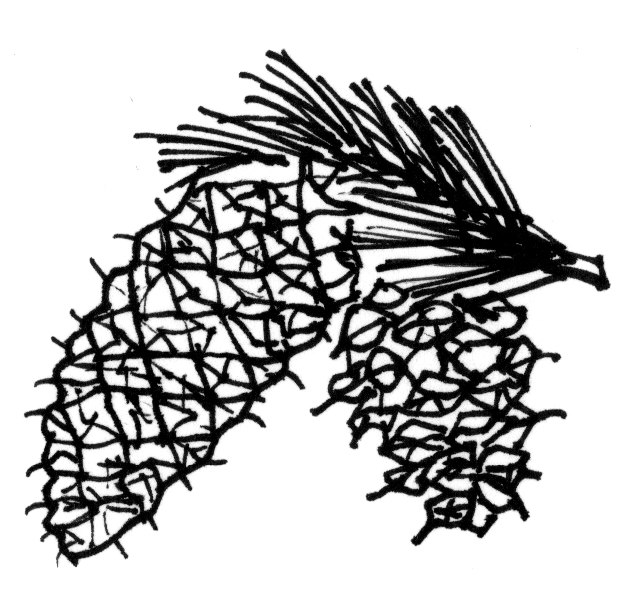
\includegraphics[width=2cm]{./abeto.jpg}
\end{center}
\clearpage
\thispagestyle{empty}

\movetoevenpage
\small\MyriadPro\itshape
\label{colaboradores}

\noindent{}COLABORADORES\\

\noindent{}MOISSEI MOUNTIAN, nascido na Moldávia (\scalebox{.8}{URSS}), é formado em engenharia civil. Em 1972, mudou"-se com sua esposa, Sofia Mountian, para o Brasil,
onde em 2008 fundou com sua filha Daniela a editora Kalinka e começou a
trabalhar como tradutor. É parte do conselho editorial da Kalinka, tendo
trazido nomes como Fiódor Sologub, Leonid Dobýtchin e Friedrich
Gorenstein aos leitores brasileiros. Foi indicado duas vezes ao Prêmio
Jabuti pelas traduções de {\slsc{O diabo mesquinho}}, de Fiódor Sologub
(Kalinka, 2008) e {\slsc{“Os sonhos teus vão acabar contigo”: prosa,
poesia, teatro}}, de Daniil Kharms (Kalinka, 2103, com Aurora Fornoni
Bernardini e Daniela Mountian). Também traduziu {\slsc{Encontros com Liz
e outras histórias}}, de Leonid Dobýtchin (Kalinka, 2009), {\slsc{Diário
de um escritor (1873): Meia carta de um sujeito}}, de Fiódor Dostoiévski
(Hedra, 2016), e {\slsc{A ressurreição do lariço: Contos de Kolimá 5}}, de
Varlam Chalámov (Ed. 34, 2016), os dois últimos em parceria com Daniela.
Com Irineu Franco Perpetuo verteu {\slsc{Salmo}}, de Friedrich Gorenstein
(indicado ao prêmio de tradução “Lendo a Rússia”, do Instituto de
Tradução de Moscou).

\medskip

\noindent{}DANIELA MOUNTIAN é tradutora, designer e criadora da Kalinka, de­dicada
à cultura russa. Fez pela \scalebox{0.8}{USP} graduação em história, mestrado sobre
Fiódor Sologub e doutorado"-sanduíche sobre Daniil Kharms, com estágio de
um ano na Casa de Púchkin, em São Petersburgo. Atualmente é
pós"-doutoranda do Departamento de Teoria Literária e Literatura
Comparada (\scalebox{0.8}{USP}), com apoio da \scalebox{0.8}{FAPESP} (processo 2017/24139-9), com a pesquisa “Literatura infantil
russa e brasileira: uma análise comparada (1919-1943)”. Além dos livros
vertidos em parceria com Moissei Mountian, traduziu com Yulia Mikaelian
{\slsc{O ofício}} e {\slsc{O compromisso}}, ambos de Serguei Dovlátov
(Kalinka, 2017, 2019).


\medskip

\noindent{}VALÉRI NIKOLÁIEVITCH SÁJIN, nascido em 1946 em Leningrado, é crítico
literário, autor de livros e artigos sobre literatura e cultura russa
dos séculos \scalebox{.8}{XVIII} ao \scalebox{.8}{XX}.
Membro da União dos Escritores de São
Petersburgo desde 1994. Enquanto estudava na escola da juventude
operária, trabalhou, entre 1961 e 1964, como serralheiro ferramenteiro
numa fábrica de equipamentos radiotécnicos. A partir de 1964 cursou a
Faculdade de Língua e Literatura Russa do Instituto Pedagógico Estatal
de Leningrado A. I. Herzen, finalizada em 1968. Entre 1968 e 1992 (com
intervalo para o serviço militar de 1969 a 1970) foi colaborador
científico do Departamento de Manuscritos da Biblioteca Pública Estatal
M. E. Saltykóv"-Schedrin (atual Biblioteca Nacional da Rússia). De 1998 a
2001 foi coeditor da revista {\slsc{Trimestre da cultura e filologia
russa}}. É autor dos livros: {\slsc{Livros de verdade amarga}} (Moscou, ed.
{\slsc{Kniga}}, 1989); {\slsc{Força do destino. Uma crônica documental do
ano 1861}} (São Petersburgo, {\slsc{Aleteia}}, 2010). Organizou as
primeiras {\slsc{Obras completas de Daniil Kharms}} em seis tomos (São
Petersburgo, {\slsc{Akademítcheskoi Proiekt}}, 1997-2001) e várias
coletâneas de suas obras; uma coletânea de poemas de B. Ch. Okudjava
(série Biblioteca do Poeta, São Petersburgo, {\slsc{Akademítcheskoi
Proiekt}}, 2001); as {\slsc{Obras completas de I. S. Barkóv}} (série
Biblioteca do Poeta, São Petersburgo, {\slsc{Akademítcheskoi Proiekt}},
2004); a coletânea das obras de L. S. Lipávski {\slsc{Estudo do terror}}
(Moscou, {\slsc{Ad Marginem}}, 2005); {\slsc{Diário de L. V. Chapórina}} em
2 tomos (Moscou, {\slsc{Nóvoie Literatúrnoie Obozriénie}}, 2012); e em
parceria com A. L. Dmitrenko o livro {\slsc{Daniil Kharms pelo olhar de
seus contemporâneos: Reminiscências. Diários. Cartas}} (São Petersburgo,
Vita Nova, 2019).

\medskip

\noindent{}KARINA AOKI é formada em arquitetura pela \scalebox{.8}{FAU-USP}. Atuou como diretora de arte e coordenadora de estúdio da São Paulo Criação – Rafic Farah
durante 8 anos, atendendo clientes como Mitsubishi Motors do Brasil,
Fundação Roberto Marinho, Fast Shop, Casa do Saber, Escola da Cidade,
Museu de Arte Brasileira da \scalebox{.8}{FAAP}, restaurantes Arabia, Spot e Ritz,
marcas de moda Maria Bonita, Mandi, Lucy in the Sky e Brooksfield Donna,
cinema \scalebox{.8}{HSBC}/Belas Artes, e o designer Carlos Motta. Foi também editora
de arte da revista {\slsc{Casa Vogue}} (Edições Globo Condé Nast) por 6 anos e
supervisora de arte do departamento de literatura da editora \scalebox{.8}{FTD}
Educação, sendo responsável por cerca de 70 títulos. Atualmente
desenvolve projetos independentes nas áreas de identidade visual,
embalagem, expografia e editorial.

\medskip

\noindent{}PAULO HENRIQUE POMPERMAIER é graduado em Jornalismo pela Faculdade Cásper Líbero e graduando em Letras pela \scalebox{0.8}{USP}. Como repórter atuou na Revista {\slsc{Cult}} e atualmente é editor"-assistente da Hedra.

\afterpage{\blankpage}

\newpage
\pagestyle{empty}
\MyriadPro

\footnotesize{
\noindent{}CATÁLOGO DA EDITORA KALINKA\\[5pt]

\noindent{}O Diabo Mesquinho\\
FIÓDOR SOLOGUB
\medskip

\noindent{}Encontros com Liz e outras histórias\\
LEONID DOBÝTCHIN
\medskip

\noindent{}“Os sonhos teus vão acabar contigo”: prosa, poesia, teatro\\
DANIIL KHARMS
\medskip

\noindent{}Luminescência: antologia poética\\
VIATCHESLÁV KUPRIYÁNOV
\medskip

\noindent{}Luminescência: desdobramentos\\
VIATCHESLÁV KUPRIYÁNOV
\medskip

\noindent{}Poesia russa: seleta bilíngue
\medskip

\noindent{}Tarakã, o bigodudo (Ars et Vita e Kalinka)\\
KORNEI TCHUKÓVSKI
\medskip

\noindent{}Parque Cultural\\
SERGUEI DOVLÁTOV
\medskip

\noindent{}Salmo\\
FRIEDRICH GORENSTEIN
\medskip

\noindent{}O ofício\\
SERGUEI DOVLÁTOV
\medskip

\noindent{}O elefante (Coleção Mir)\\
ALEKSANDR KUPRIN
\medskip

\noindent{}A velha (Coleção Mir)\\
DANIIL KHARMS 
\medskip

\noindent{}Bobók \& ‘Meia carta’ de sujeito (Coleção Mir)\\
FIÓDOR DOSTOIÉVSKI
\medskip

\noindent{}Aulas de literatura russa: de Púchkin a Gorenstein \\
AURORA FORNONI BERNARDINI
\medskip

\noindent{}O compromisso\\
SERGUEI DOVLÁTOV
\medskip

\noindent{}A cidade Ene \\
LEONID DOBÝTCHIN
}

\newpage
\pagestyle{empty}
\MyriadPro
\scriptsize
\begin{center}
GOROD EN\\[6pt]

Copyright © Kalinka, 2020\\[6pt]

Tradução © Moissei Mountian, Daniela Mountian, 2020\\[6pt]

Prefácio © Valéri Sájin, 2019\\[6pt]

primeira edição, 2020\\[40pt]


Essa publicação está de acordo com a reforma ortográfica.\\[6pt]
A versão se baseou no livro {\slsc{Leonid Dobýtchin: zabýtaia kniga}} (Moscou: {\slsc{Khudójestvenaia literatura}}, 1989), organizado por Víktor Eroféiev.\\[6pt]	
%A imagem que precede o posfácio é baseada em autocharge do autor.\\[20pt]
\end{center}


\bigskip

\begin{vplace}[1]
\begin{table}[ht!]
\centering
\MyriadPro\itshape
\scriptsize
\begin{tabular}{rl}
TÍTULO            & A cidade Ene 									   \\[2pt]
AUTOR             & Leonid Dobýtchin                          		   \\[2pt]
TRADUÇÃO do RUSSO & Moissei e Daniela Mountian		                   \\[2pt]
PREFÁCIO          & Valéri Sájin	                                   \\[2pt]
CAPA              & Karina Aoki		                                   \\[2pt]
PROJETO GRÁFICO   & Kalinka                                            \\[2pt]
PRODUÇÃO EXECUTIVA & Hedra                                             \\[2pt]
EDIÇÃO            & Kalinka 		                                   \\[2pt] 
EDITOR-ASSISTENTE & Paulo Henrique Pompermaier                         \\[2pt] 
FORMATO           & 14 x 21 cm                                         \\[2pt]
NÚMERO de PÁGINAS & XXX                                                \\[2pt]
ISBN              & 978-85-XXXXX-XX-X                                 
\end{tabular}
\end{table}
\end{vplace}

\newpage
\MyriadPro\itshape
\begin{center}
\small
A cidade Ene

Город Эн
\end{center}

\scriptsize


%\begin{figure}[!ht]
%%\begin{minipage}{2\textwidth}
%\centering
%
  %\includegraphics[width=80mm]{./imgs/ficha.jpg}
%%\caption{I}
%%\end{minipage}
 %\end{figure}


%\begin{vplace}[1]
%\begin{center}
%Dados Internacionais de Catalogação na Publicação (CIP)\\
%(Câmara Brasileira do Livro, SP, Brasil)\\
%\_\_\_\_\_\_\_\_\_\_\_\_\_\_\_\_\_\_\_\_\_\_\_\_\_\_\_\_\_\_\_\_\_\_\_\_\_\_\_\_\_\_\_\_\_\_\_\_\_\_\_\_\_\_\_\_\_\_\_\\
%\end{center}
%\hspace{30pt}Bernardini, Aurora Fornoni, XXXX--


%\hspace{35pt}Aulas de literatura russa : de Púchkin a Gorenstein / Aurora Fornoni

%\hspace{12pt}Bernardini ; organização Valteir Vaz ; prefácio Arlete Cavaliere. - - São Paulo :

%\hspace{12pt}Kalinka, 2018.\\[6pt]

%\hspace{35pt}ISBN XXX-XX-XXXXX-XX-X\\[6pt]

%\hspace{35pt}1. Literatura russa II. Crítica literária III. Título.

%\begin{center}
%\hspace{10pt}XX-XXXXX \hspace{180pt}CDD-XXX.X
%\_\_\_\_\_\_\_\_\_\_\_\_\_\_\_\_\_\_\_\_\_\_\_\_\_\_\_\_\_\_\_\_\_\_\_\_\_\_\_\_\_\_\_\_\_\_\_\_\_\_\_\_\_\_\_\_\_\_\_\\
%Índices para catálogo sistemático:\\[3pt]
%1. Crítica literária : Literatura russa XXX.X\\
%\end{center}
%\end{vplace}
\vfill
\begin{center}
EDIÇÃO: EDITORA KALINKA\\[7pt]
Rua Imaculada Conceição, 41 cj. 03\\[7pt]
01226-020 São Paulo-SP Tel.11 2579-6290\\[7pt]
www.kalinka.com.br\\[30pt]

PRODUÇÃO EXECUTIVA: EDITORA HEDRA\\[7pt]
Rua Fradique Coutinho, 1139 Vila Madalena\\[7pt]
05416-011 São Paulo-SP Tel.11 3097-8304\\[7pt]
www.hedra.com.br
\end{center}
%TÍTULO Aulas de literatura russa: de Púchkin a Gorenstein\\
%AUTOR Aurora Fornoni Bernardini\\
%REVISÃO Daniela Mountian e Paulo Henrique Pompermaier\\
%EDIÇÃO Hedra\\
%CAPA Daniela Mountian\\
%PROJETO GRÁFICO Hedra\\
%FORMATO 14 x 21 cm\\
%NÚMERO de PÁGINAS 398\\
%ISBN XXX-XX-XXXXX-XX-X\\

\end{document}
